\documentclass[UTF8,nofonts,mathserif]{beamer}
\usepackage{beamerthemeshadow}
\usepackage{beamerthemesplit}
\usepackage[noindent,nofonts]{ctexcap} 
\setCJKmainfont[BoldFont=STHeiti]{STXihei} 
%\setromanfont{SimSun} 

\usepackage{xcolor}

%\usetheme{shadow}
\usecolortheme{default}
\setbeamertemplate{footline}[frame number]
\useinnertheme[shadow=true]{rounded}
%\setbeamertemplate{footline}{\insertframenumber/\inserttotalframenumber}
%\useoutertheme{infolines}
%\setbeamertemplate{headline}{} % removes the headline that infolines inserts

%\usetheme{boxes}
%\usepackage{amsmass}
%\usepackage{amssymb,amsfonts,url}

\usepackage{algorithm}
\usepackage{algorithmic}

\usepackage{geometry}
\geometry{top=2cm,left=3cm,bottom=2cm,right=3cm}

\usepackage{graphicx}
\graphicspath{{Problems/}}

\usepackage{tikz}
\usetikzlibrary{shadows}
\usetikzlibrary{positioning}
\usepackage{verbatim}
\usepackage{pgfplots}
\usepackage{verbatim}
\usetikzlibrary{arrows,shapes}

\definecolor{darkblue}{rgb}{0.2,0.2,0.6}
\definecolor{darkred}{rgb}{0.6,0.1,0.1}
\definecolor{darkgreen}{rgb}{0.2,0.6,0.2}

% def circled nums
\newcommand*\circled[1]{\tikz[baseline=(char.base)]{
            \node[shape=circle,draw,inner sep=2pt] (char) {#1};}}

\usetikzlibrary{shadings,shadows,shapes.arrows}

\usetikzlibrary{calc} 
\makeatletter 
\@namedef{color@3}{blue!20}
\@namedef{color@1}{green!70}   
%\@namedef{color@3}{yellow!50} 
\@namedef{color@2}{orange!90}  
%\@namedef{color@5}{magenta!70} 
%\@namedef{color@6}{yellow!70}    

\newcommand{\graphitemize}[2]{%
\begin{tikzpicture}[every node/.style={align=center}, scale=0.78]  
 \draw[fill=green!5, fill opacity=0.1, green, inner sep=0.05cm, outer sep=0.05cm] (5,0) arc(0:360:5);
 % \draw[fill=white, fill opacity=0.1, white, inner sep=0.05cm, outer sep=0.05cm] (4,0) arc(0:360:4);
%  \shade[ball color=gray!10!] (0,0) coordinate(Hp) circle (.9);
  \node[shape=circle,  minimum size=1.1cm,fill=red!60,font=\Large,outer sep =.15cm,inner sep=.2cm,drop  shadow={ashadow, color=yellow}](ce){#1};  
   % \shade[ball color=blue!20!] (0,0) coordinate($Algorithm$) circle (1.5cm);

\foreach \gritem [count=\xi] in {#2}  {\global\let\maxgritem\xi}  
\foreach \gritem [count=\xi] in {#2}
{% 
\pgfmathtruncatemacro{\angle}{90+360/\maxgritem*\xi}
\edef\col{\@nameuse{color@\xi}}
\node[shape=circle,
     ultra thick,
     draw=white,
     fill opacity=1,
     drop  shadow={ashadow, color=blue!60},
     fill=\col,outer sep=0.25cm,        
     minimum size=2cm] (satellite-\xi) at (\angle:5cm) {\gritem };
     \draw[line width=0.25cm,-latex, \col] (ce) -- (satellite-\xi);
     }%
% \draw[violet, fill=violet!10] (4,0) arc(0:360:4);
\end{tikzpicture}  
}%



\newcommand*{\tikzarrow}[2]{%
  \tikz[
    baseline=(A.base),             % Set baseline to the baseline of node content
    font=\footnotesize\sffamily    % Set fontsize of the node content
  ]
  \node[
    single arrow,                  % Shape of the node
    single arrow head extend=2pt,  % Actual width of arrow head
    draw,                          % Draw the node shape
    inner sep=2pt,                 % Separation between node content and node shape
    top color=white,               % Shading color on top of node
    bottom color=#1,               % Shading color on bottom of node
    drop shadow                    % Draw a shadow
  ] (A) {#2};%
}


\def\arrow{
  (10.05:1.1) -- (6.05:1) arc (6.05:120:1) [rounded corners=0.5] --
  (120:0.9) [rounded corners=1] -- (130:1.1) [rounded corners=0.5] --
  (120:1.3) [sharp corners] -- (120:1.2) arc (120:5.25:1.2)
  [rounded corners=1] -- (10.05:1.1) -- (6.05:1) -- cycle
}

\tikzset{
  ashadow/.style={opacity=.25, shadow xshift=0.07, shadow yshift=-0.07},
}

\def\arrows[#1]{         
  \begin{scope}[scale=#1]
    \draw[color=darkred, drop  shadow={ashadow, color=red!60!black}] \arrow;

    \draw[color=darkgreen, bottom color=green!90!black, top color=green!60,   drop shadow={ashadow, color=green!60!black}] [rotate=120] \arrow;

    \draw[color=darkblue, right color=blue, left color=blue!60,   drop shadow={ashadow, color=blue!60!black}] [rotate=240] \arrow;

    % to hide the green shadow
    \draw[color=darkred, left color=red, right color=red!60] \arrow;
  \end{scope}
}

\tikzstyle{vertex}=[circle,fill=black!25,draw,minimum size=20pt,inner sep=0pt]
\tikzstyle{middlevertex}=[circle,fill=black!25,draw,minimum size=15pt,inner sep=0pt]
\tikzstyle{smallvertex}=[circle,fill=black!25,draw,minimum size=10pt,inner sep=0pt]
\tikzstyle{tinyvertex}=[circle,fill=black!25,draw,minimum size=5pt,inner sep=0pt]
\tikzstyle{selected vertex} = [vertex, draw,fill=yellow!24]
\tikzstyle{blue smallvertex} = [smallvertex, draw,fill=blue]
\tikzstyle{red smallvertex} = [smallvertex, draw,fill=yellow]
\tikzstyle{edge} = [draw,thick,->]
\tikzstyle{undirectededge} = [draw,thick]
\tikzstyle{weight} = [font=\small]
\tikzstyle{selected edge} = [draw,line width=3pt,-,red!50]
\tikzstyle{ignored edge} = [draw,line width=3pt,-,black!20]
\tikzstyle{squarednode}=[draw, fill=blue!20, thick, minimum size=5mm]
\tikzstyle{roundnode}=[circle, draw, fill=blue!20, thick, minimum size=5mm]

\tikzset{nd/.style={rectangle,draw,align=center}}

\title{Figures used in CS711008Z  Algorithm Design and Analysis: Part 2 }
\author{Dongbo Bu }
\institute{ {\small Institute of Computing Technology \\
Chinese Academy of Sciences, Beijing, China}}




\date{}



\begin{document}

\frame{
	\frametitle{Banded DP}
	
	
\begin{figure}[h]\centering
    
 \begin{tikzpicture}[scale=0.89, auto,swap]
  
  	\def\d{0.7};
	
	%draw index 
 \def\dy{1};
 \def\dx{0};

    \foreach \i/\num/\name in {0/Y:\ /, 1/''/s1,2/O/s2,3/C/s3,4/U/s4,5/R/,6/R/,7/A/,8/N/,9/C/,10/E/}{
           \node[blue,thick] (\name) at (\i*\d+\d/2 + \dx*\d - \d, \d/2 + \dy * \d) {\tt \num};
    }

%    \foreach \i/\num/\name in {0/Y:\ /}{
%           \node[blue,thick] (\name) at (\i*\d+\d/2 + \dx*\d - \d, \d/2 + \dy * \d) {$\mathrm{\num}$};
%    }


 \def\dy{0};
 \def\dx{0};
    \foreach \i/\num/\name in {1/X:''/s1,2/O/s2,3/C/s3,4/C/s4, 5/U/,6/R/,7/R/,8/E/,9/N/,10/C/,11/E/}{
         \node[blue,thick] (\name) at ( -1*\d+\d/2  - 0.3,  0.0 - \i*\d + \d/2 - \dy * \d + \d){\tt  \num};
    }

%    \foreach \i/\num/\name in {1/X:''/s1 }{
%         \node[blue,thick] (\name) at ( -1*\d+\d/2  - 0.3,  0.0 - \i*\d + \d/2 - \dy * \d + \d){ $\mathrm{ \num}$};
%    }
%
    
%score	
 \def\dy{0};
 \def\dx{0};
    \foreach \i/\num/\name in {0/0/LU,1/1/U,2/2/S2,3/3/,4/4/,5/5/,6/6/,7/7/,8/8/,9/9/}{
             \draw[  thick ] (\i*\d + \dx*\d,  0+ \dy*\d) rectangle (\i*\d+\d + \dx*\d, \d + \dy*\d);
         \node (\name) at (\i*\d+\d/2 + \dx*\d, \d/2 + \dy*\d) {\tiny $\num$};
    }


 \def\dy{-1};
 \def\dx{0};
    \foreach \i/\num/\name in {0/1/L,1/0/C,2/1/,3/2/,4/3/,5/4/,6/5/,7/6/,8/7/,9/8/}{
             \draw[  thick ] (\i*\d + \dx*\d,  0+ \dy*\d) rectangle (\i*\d+\d + \dx*\d, \d + \dy*\d);
         \node (\name) at (\i*\d+\d/2 + \dx*\d, \d/2 + \dy*\d) {\tiny $\num$};
    }
    
%
%   \draw[red,ultra thick] (C) circle[radius=\d/2];
%   \draw[blue,ultra thick] (U) circle[radius=\d/2];
%   \draw[blue,ultra thick] (LU) circle[radius=\d/2];
%   \draw[blue,ultra thick] (L) circle[radius=\d/2];                                

   
        
 \def\dy{-2};
 \def\dx{0};
    \foreach \i/\num/\name in {0/2/,1/1/,2/0/,3/1/L,4/2/C,5/3/,6/4/,7/5/,8/6/,9/7/}{
             \draw[  thick ] (\i*\d + \dx*\d,  0+ \dy*\d) rectangle (\i*\d+\d + \dx*\d, \d + \dy*\d);
         \node (\name) at (\i*\d+\d/2 + \dx*\d, \d/2 + \dy*\d) {\tiny $\num$};
    }
    



    
 \def\dy{-3};
 \def\dx{0};
    \foreach \i/\num/\name in {0/3/,1/2/,2/1/,3/1/S3,4/2/,5/3/,6/4/,7/5/,8/5/,9/6/}{
             \draw[  thick ] (\i*\d + \dx*\d,  0+ \dy*\d) rectangle (\i*\d+\d + \dx*\d, \d + \dy*\d);
         \node (\name) at (\i*\d+\d/2 + \dx*\d, \d/2 + \dy*\d) {\tiny $\num$};
    }
    
  \def\dy{-4};
 \def\dx{0};
    \foreach \i/\num/\name in {0/4/,1/3/,2/2/,3/1/S3,4/2/,5/3/,6/4/,7/5/,8/6/,9/6/}{
             \draw[  thick ] (\i*\d + \dx*\d,  0+ \dy*\d) rectangle (\i*\d+\d + \dx*\d, \d + \dy*\d);
         \node (\name) at (\i*\d+\d/2 + \dx*\d, \d/2 + \dy*\d) {\tiny $\num$};
    }
    
  \def\dy{-5};
 \def\dx{0};
    \foreach \i/\num/\name in {0/5/,1/4/,2/3/,3/2/S3,4/1/,5/2/,6/3/,7/4/,8/5/,9/6/}{
             \draw[  thick ] (\i*\d + \dx*\d,  0+ \dy*\d) rectangle (\i*\d+\d + \dx*\d, \d + \dy*\d);
         \node (\name) at (\i*\d+\d/2 + \dx*\d, \d/2 + \dy*\d) {\tiny $\num$};
    }
    
  \def\dy{-6};
 \def\dx{0};
    \foreach \i/\num/\name in {0/6/,1/5/,2/4/,3/3/S3,4/2/,5/1/,6/2/,7/3/,8/4/,9/5/}{
             \draw[  thick ] (\i*\d + \dx*\d,  0+ \dy*\d) rectangle (\i*\d+\d + \dx*\d, \d + \dy*\d);
         \node (\name) at (\i*\d+\d/2 + \dx*\d, \d/2 + \dy*\d) {\tiny $\num$};
    }
    
  \def\dy{-7};
 \def\dx{0};
    \foreach \i/\num/\name in {0/7/,1/6/,2/5/,3/4/S3,4/3/,5/2/,6/2/,7/3/,8/4/,9/4/}{
             \draw[  thick ] (\i*\d + \dx*\d,  0+ \dy*\d) rectangle (\i*\d+\d + \dx*\d, \d + \dy*\d);
         \node (\name) at (\i*\d+\d/2 + \dx*\d, \d/2 + \dy*\d) {\tiny $\num$};
    }
    
  \def\dy{-8};
 \def\dx{0};
    \foreach \i/\num/\name in {0/8/,1/7/,2/6/,3/5/S3,4/4/,5/3/,6/3/,7/2/,8/3/,9/4/}{
             \draw[  thick ] (\i*\d + \dx*\d,  0+ \dy*\d) rectangle (\i*\d+\d + \dx*\d, \d + \dy*\d);
         \node (\name) at (\i*\d+\d/2 + \dx*\d, \d/2 + \dy*\d) {\tiny $\num$};
    }
    
  \def\dy{-9};
 \def\dx{0};
    \foreach \i/\num/\name in {0/9/,1/8/,2/7/,3/6/S3,4/5/,5/4/,6/4/,7/3/,8/2/LU,9/3/U}{
             \draw[  thick ] (\i*\d + \dx*\d,  0+ \dy*\d) rectangle (\i*\d+\d + \dx*\d, \d + \dy*\d);
         \node (\name) at (\i*\d+\d/2 + \dx*\d, \d/2 + \dy*\d) {\tiny $\num$};
    }
    
  \def\dy{-10};
 \def\dx{0};
    \foreach \i/\num/\name in {0/10/,1/9/,2/8/,3/7/S3,4/6/,5/5/,6/5/,7/4/,8/3/L,9/2/C}{
             \draw[  thick ] (\i*\d + \dx*\d,  0+ \dy*\d) rectangle (\i*\d+\d + \dx*\d, \d + \dy*\d);
         \node (\name) at (\i*\d+\d/2 + \dx*\d, \d/2 + \dy*\d) {\tiny $\num$};
    }
    
%    
%           \draw[red,ultra thick] (C) circle[radius=\d/2];
%   \draw[blue,ultra thick] (U) circle[radius=\d/2];
%   \draw[blue,ultra thick] (LU) circle[radius=\d/2];
%   \draw[blue,ultra thick] (L) circle[radius=\d/2];                                

	\node at ( 5*\d+\d/2 + \dx*\d, \d/2 + -11*\d) {\small $(a)$};
%
%\end{tikzpicture} 
%\label{NeedlemanWunschExample}
%\caption{\fangsong {\sc Needleman-Wunsch}算法计算字符串$\mathrm{x}$和$\mathrm{y}$的最优联配运行过程示例:字符串$T=\text{\tt "OCCURRENCE"}$, $S=\text{\tt "OCURRANCE"}$。}
%\end{figure}     
%
%
%
%
%
%\begin{figure}\centering
%    
% \begin{tikzpicture}[scale=0.9, auto,swap]
%  
	
  	\def\d{0.7};
	
	%draw index 
 \def\dy{1};
 \def\dx{10.5};

    \foreach \i/\num/\name in { 1/''/,2/O/s2,3/C/s3,4/U/s4,5/R/,6/R/,7/A/,8/N/,9/C/,10/E/}{
           \node[blue,thick] (\name) at (\i*\d+\d/2 + \dx*\d - \d, \d/2 + \dy * \d) {\tt \num};
    }


%    \foreach \i/\num/\name in {0/S:\ /, 1/''/,2/O/s2,3/C/s3,4/U/s4,5/R/,6/R/,7/A/,8/N/,9/C/,10/E/}{
%           \node[blue,thick] (\name) at (\i*\d+\d/2 + \dx*\d - \d, \d/2 + \dy * \d) {\tt \num};
%    }
%
%
% \def\dy{0};
% \def\dx{10.5};
%    \foreach \i/\num/\name in {1/T:''/s1,2/O/s2,3/C/s3,4/C/s4, 5/U/,6/R/,7/R/,8/E/,9/N/,10/C/,11/E/}{
%         \node[blue,thick] (\name) at ( -1*\d+\d/2  - 0.3,  0.0 - \i*\d + \d/2 - \dy * \d + \d){\tt  \num};
%    }
%
    
%score	

%yellow box 
 \def\dy{-1};
 \def\dx{10.5};
    \foreach \i/\j/\name in {0/0/L,1/1/C,2/2/,2/3/,3/4/,4/5/,5/6/,6/7/,7/8/,8/9/,9/10}{
             \draw[ fill=yellow, thick ] (\i*\d + \dx*\d,  0+ \dy*\j*\d) rectangle (\i*\d+\d + \dx*\d, \d + \dy*\j*\d);
    }



 \def\dy{0};
 \def\dx{10.5};
    \foreach \i/\num/\name in {0/0/A11,1/1/A12,2/2/A13,3/3/A14,4/4/A15,5/5/A16,6/6/A17,7/7/A18,8/8/A19,9/9/A110}{
             \draw[  thick ] (\i*\d + \dx*\d,  0+ \dy*\d) rectangle (\i*\d+\d + \dx*\d, \d + \dy*\d);
         \node (A0\i) at (\i*\d+\d/2 + \dx*\d, \d/2 + \dy*\d) {\tiny $\num$};
    }


 \def\dy{-1};
 \def\dx{10.5};
    \foreach \i/\num/\name in {0/1/L,1/0/C,2/1/,3/2/,4/3/,5/4/,6/5/,7/6/,8/7/,9/8/}{
             \draw[  thick ] (\i*\d + \dx*\d,  0+ \dy*\d) rectangle (\i*\d+\d + \dx*\d, \d + \dy*\d);
         \node (A1\i) at (\i*\d+\d/2 + \dx*\d, \d/2 + \dy*\d) {\tiny $\num$};
    }
    
   
        
 \def\dy{-2};
 \def\dx{10.5};
    \foreach \i/\num/\name in {0/2/,1/1/,2/0/,3/1/L,4/2/C,5/3/,6/4/,7/5/,8/6/,9/7/}{
             \draw[  thick ] (\i*\d + \dx*\d,  0+ \dy*\d) rectangle (\i*\d+\d + \dx*\d, \d + \dy*\d);
         \node (A2\i) at (\i*\d+\d/2 + \dx*\d, \d/2 + \dy*\d) {\tiny $\num$};
    }
    



    
 \def\dy{-3};
 \def\dx{10.5};
    \foreach \i/\num/\name in {0/3/,1/2/,2/1/,3/1/S3,4/2/,5/3/,6/4/,7/5/,8/5/,9/6/}{
             \draw[  thick ] (\i*\d + \dx*\d,  0+ \dy*\d) rectangle (\i*\d+\d + \dx*\d, \d + \dy*\d);
         \node (A3\i) at (\i*\d+\d/2 + \dx*\d, \d/2 + \dy*\d) {\tiny $\num$};
    }
    
  \def\dy{-4};
 \def\dx{10.5};
    \foreach \i/\num/\name in {0/4/,1/3/,2/2/,3/1/S3,4/2/,5/3/,6/4/,7/5/,8/6/,9/6/}{
             \draw[  thick ] (\i*\d + \dx*\d,  0+ \dy*\d) rectangle (\i*\d+\d + \dx*\d, \d + \dy*\d);
         \node (A4\i) at (\i*\d+\d/2 + \dx*\d, \d/2 + \dy*\d) {\tiny $\num$};
    }
    
  \def\dy{-5};
 \def\dx{10.5};
    \foreach \i/\num/\name in {0/5/,1/4/,2/3/,3/2/S3,4/1/,5/2/,6/3/,7/4/,8/5/,9/6/}{
             \draw[  thick ] (\i*\d + \dx*\d,  0+ \dy*\d) rectangle (\i*\d+\d + \dx*\d, \d + \dy*\d);
         \node (A5\i) at (\i*\d+\d/2 + \dx*\d, \d/2 + \dy*\d) {\tiny $\num$};
    }
    
  \def\dy{-6};
 \def\dx{10.5};
    \foreach \i/\num/\name in {0/6/,1/5/,2/4/,3/3/S3,4/2/,5/1/,6/2/,7/3/,8/4/,9/5/}{
             \draw[  thick ] (\i*\d + \dx*\d,  0+ \dy*\d) rectangle (\i*\d+\d + \dx*\d, \d + \dy*\d);
         \node (A6\i) at (\i*\d+\d/2 + \dx*\d, \d/2 + \dy*\d) {\tiny $\num$};
    }
    
  \def\dy{-7};
 \def\dx{10.5};
    \foreach \i/\num/\name in {0/7/,1/6/,2/5/,3/4/S3,4/3/,5/2/,6/2/,7/3/,8/4/,9/4/}{
             \draw[  thick ] (\i*\d + \dx*\d,  0+ \dy*\d) rectangle (\i*\d+\d + \dx*\d, \d + \dy*\d);
         \node (A7\i) at (\i*\d+\d/2 + \dx*\d, \d/2 + \dy*\d) {\tiny $\num$};
    }
    
  \def\dy{-8};
 \def\dx{10.5};
    \foreach \i/\num/\name in {0/8/,1/7/,2/6/,3/5/S3,4/4/,5/3/,6/3/,7/2/,8/3/,9/4/}{
             \draw[  thick ] (\i*\d + \dx*\d,  0+ \dy*\d) rectangle (\i*\d+\d + \dx*\d, \d + \dy*\d);
         \node (A8\i) at (\i*\d+\d/2 + \dx*\d, \d/2 + \dy*\d) {\tiny $\num$};
    }
    
  \def\dy{-9};
 \def\dx{10.5};
    \foreach \i/\num/\name in {0/9/,1/8/,2/7/,3/6/S3,4/5/,5/4/,6/4/,7/3/,8/2/LU,9/3/U}{
             \draw[  thick ] (\i*\d + \dx*\d,  0+ \dy*\d) rectangle (\i*\d+\d + \dx*\d, \d + \dy*\d);
         \node (A9\i) at (\i*\d+\d/2 + \dx*\d, \d/2 + \dy*\d) {\tiny $\num$};
    }
    
  \def\dy{-10};
 \def\dx{10.5};
    \foreach \i/\num/\name in {0/10/,1/9/,2/8/,3/7/S3,4/6/,5/5/,6/5/,7/4/,8/3/L,9/2/C}{
             \draw[  thick ] (\i*\d + \dx*\d,  0+ \dy*\d) rectangle (\i*\d+\d + \dx*\d, \d + \dy*\d);
         \node (A10\i) at (\i*\d+\d/2 + \dx*\d, \d/2 + \dy*\d) {\tiny $\num$};
    }
    

	\foreach \i\j in {10/9, 9/8, 8/7, 7/6, 6/5, 5/4, 4/3, 3/2, 2/1, 1/0} {
		\draw[->, blue] (A\i0) to (A\j0);
	}
	
	\foreach \i\j in {9/8, 8/7, 7/6, 6/5, 5/4, 4/3, 3/2, 2/1, 1/0} {
		\draw[->, blue] (A0\i.120) to (A0\j.60);
	}

	\foreach \i\j in {10/9, 9/8, 8/7, 7/6, 6/5, 5/4, 4/3, 3/2, 2/1} {
		\draw[->, blue] (A\i1) to (A\j1);
	}
	\foreach \i\j in {10/9, 9/8, 8/7, 7/6, 6/5, 5/4, 4/3} {
		\draw[->, blue] (A\i2) to (A\j2);
	}
	\foreach \i\j in {10/9, 9/8, 8/7, 7/6, 6/5, 5/4} {
		\draw[->, blue] (A\i3) to (A\j3);
	}
	\foreach \i\j in {10/9, 9/8, 8/7, 7/6, 6/5} {
		\draw[->, blue] (A\i4) to (A\j4);
	}
	\foreach \i\j in {10/9, 9/8, 8/7, 7/6} {
		\draw[->, blue] (A\i5) to (A\j5);
	}
	\foreach \i\j in {10/9, 9/8, 8/7} {
		\draw[->, blue] (A\i6) to (A\j6);
	}
	\foreach \i\j in {10/9, 9/8} {
		\draw[->, blue] (A\i7) to (A\j7);
	}
	\foreach \i\j in {10/9} {
		\draw[->, blue] (A\i8) to (A\j8);
	}

	\foreach \i\j in {9/8, 8/7, 7/6, 6/5, 5/4, 4/3, 3/2, 2/1} {
		\draw[->, blue] (A1\i.120) to (A1\j.60);
	}
	\foreach \i\j in {9/8, 8/7, 7/6, 6/5, 5/4, 4/3, 3/2} {
		\draw[->, blue] (A2\i.120) to (A2\j.60);
	}
	\foreach \i\j in {9/8,  7/6, 6/5, 5/4, 4/3} {
		\draw[->, blue] (A3\i.120) to (A3\j.60);
	}
	\foreach \i\j in {8/7, 7/6, 6/5, 5/4, 4/3} {
		\draw[->, blue] (A4\i.120) to (A4\j.60);
	}
	\foreach \i\j in {9/8, 8/7, 7/6, 6/5, 5/4} {
		\draw[->, blue] (A5\i.120) to (A5\j.60);
	}
	\foreach \i\j in {9/8, 8/7, 7/6, 6/5} {
		\draw[->, blue] (A6\i.120) to (A6\j.60);
	}
	\foreach \i\j in {8/7, 7/6} {
		\draw[->, blue] (A7\i.120) to (A7\j.60);
	}
	\foreach \i\j in {9/8, 8/7} {
		\draw[->, blue] (A8\i.120) to (A8\j.60);
	}
	\foreach \i\j in {9/8} {
		\draw[->, blue] (A9\i.120) to (A9\j.60);
	}
	\draw[->, blue] (A79) to (A68);
	\draw[->, blue] (A49) to (A38);
	\draw[->, blue] (A38) to (A27);
%	\draw[->, blue] (A48) to (A47);	
	\draw[->, blue] (A43) to (A32);	
	\draw[->, blue] (A33) to (A22);	

	\draw[->, red,  thick] (A109) to (A98);
	\draw[->, red,  thick] (A98) to (A87);	
	\draw[->, red,  thick] (A87) to (A76);				
		\draw[->, red,  thick] (A76) to (A65);
		\draw[->, red,  thick] (A65) to (A54);
		\draw[->, red,  thick] (A54) to (A43);
		\draw[->, red,  thick] (A43) to (A32);
		\draw[->, red,  thick] (A32) to (A22);
		\draw[->, red,  thick] (A22) to (A11);
			\draw[->, red,  thick] (A11) to (A00);
			
			
	\node at ( 5*\d+\d/2 + \dx*\d, \d/2 + -11*\d) {\small $(b)$};

 
\end{tikzpicture} 
\end{figure}

} 

\frame{
$P_{1}$ 

$P_{2}$ 

$P_{3}$ 

$P_{4}$ 

$P_{5}$ 


$x_{1} = 1$ 

$x_{1}  = 0$ 


$x_{2} = 1$ 

$x_{2}  = 0$ 


$\{P_{2}, P_{4}, P_{5}\}$
}

\frame{


\graphitemize{Algorithm}{Genome\\Assembly, Disease\\Network, Protein\\Structure}
}

\frame{


\graphitemize{ARCS}{ARCS23,$nano$ARCS,$meta$ARCS}
}



\frame{
	\frametitle{AAA}
	
	\begin{figure}[!ht]
  \centering
  \begin{tikzpicture}
  [dot/.style={circle,draw=black,fill=black,thick,inner sep=0pt,minimum size=1mm}]
  \node[dot] (11) at (0.2,0.3) {};
  \node[dot,label=above:{\tiny $A_2$}] (12) at (2,0.3) {};
  \node[dot] (13) at (3,0.3) {};
  \node[dot,label=above:{\tiny $A_4$}] (14) at (4,0.3) {};
  \node[dot] (15) at (5,0.3) {};
  \node[dot,label=above:{\tiny $A_7$}] (16) at (7,0.3) {};
  \node[dot] (17) at (8.5,0.3) {};
  \node[dot,label=above:{\tiny $A_8$}] (18) at (9,0.3) {};
  
  \node[dot] (21) at (0.15,1.1) {};
  \node[dot,label=above:{\tiny $A_1$}] (22) at (1.3,1.1) {};
  \node[dot] (23) at (1.8,1.1) {};
  \node[dot,label=above:{\tiny $A_3$}] (24) at (3.5,1.1) {};
  \node[dot] (25) at (4.6,1.1) {};
  \node[dot,label=above:{\tiny $A_5$}] (26) at (6,1.1) {};
  \node[dot] (27) at (7.8,1.1) {};
  \node[dot,label=above:{\tiny $A_9$}] (28) at (9.4,1.1) {};
  
  \node[dot] (31) at (0.2,1.9) {};
  \node[dot,label=above:{\tiny $A_6$}] (32) at (6.5,1.9) {};
  
  \draw [black,thick] (11) -- (12)node [midway,above,draw=none] {\textcolor[rgb]{1.00,0.00,0.00}{\tiny {$W_2=5$}}};
  \draw [black,thick] (13)node [above,draw=none] {\textcolor[rgb]{1.00,0.00,0.00}{\tiny {{$W_4=2$}}}} -- (14);
  \draw [black,thick] (15) -- (16) node [midway,above,draw=none] {\textcolor[rgb]{1.00,0.00,0.00}{\tiny {{$W_7=1$}}}};
  \draw [black,thick] (17) -- (18);
  
  \draw [white] (8.2,0.38) node [above,draw=none] {\textcolor[rgb]{1.00,0.00,0.00}{\tiny {{$W_8=3$}}}}-- (9,0.38);
  
  \draw [black,thick] (21)node [above,draw=none] {\textcolor[rgb]{1.00,0.00,0.00}{\tiny {$W_1=1$}}} -- (22);
  \draw [black,thick] (23) --node [above,draw=none] {\textcolor[rgb]{1.00,0.00,0.00}{\tiny {$W_3=4$}}} (24);
  \draw [black,thick] (25) node [above,draw=none] {\textcolor[rgb]{1.00,0.00,0.00}{\tiny {$W_5=3$}}}-- (26);
  \draw [black,thick] (27) node [above,draw=none] {\textcolor[rgb]{1.00,0.00,0.00}{\tiny {{$W_9=5$}}}}-- (28);
  
  \draw [black,thick] (31) -- (32) node [midway,above,draw=none] {\textcolor[rgb]{1.00,0.00,0.00}{\tiny {$W_6=2$}}};
  
  \draw [->,green,thick] (0,0) -- (9.5,0) node [right,draw=none] {\textcolor[rgb]{0.00,0.00,0.00}{$Time$}};
  \end{tikzpicture}
%  \caption{L7-intervalschedulingexample.eps}
\end{figure}


}

\frame{
	\frametitle{BBB}
	
	\begin{figure}
\begin{tikzpicture}[scale=1., auto,swap]
    % Draw a 7,11 network
    % First we draw the vertices
    \foreach \pos/\name/\label in {{(0,0)/root/}, 
    {(-3,-1)/L/}, {(3,-1)/R/}}
        \node[tinyvertex,draw=black, fill=white!20] (\name) at \pos {};
        
        
        \foreach \pos/\name/\label in {{(0.1,0)/root/P_0:\ X=[?,?,?,?,?,?,?,?,?]}, 
    {(-2.9,-1)/L/P_1:\ X=[?,?,?,?,?,?,?,?,1]}, {(3.1,-1)/R/P_2:\ X=[?,?,?,?,?,?,?,?,0]}}
        \node[right] at \pos {\tiny $\label$};    

    % Connect vertices with edges and draw weights
  \foreach \source/ \dest /\weight in {root/L/{\tiny x_9=1}, R/root/{\tiny x_9=0}}
        \path[undirectededge] (\source) -- node[ weight] {$\weight$} (\dest);
%       \draw[dashed, ->] (0,0) arc  (120:60:2);
 
   \end{tikzpicture}
\end{figure}
`
}

\frame{
	\frametitle{CCC}
	
\begin{small}
{\sc GreedyIntervalScheduling}$(CourseSet)$
\begin{algorithmic}[1]
\WHILE{$CourseSet$ $\neq \emptyset$}
\STATE{Select the course $C$ with \textcolor{red}{\bf earliest finishing time};}
\STATE Remove $C$ and related courses from $CourseSet$; 
\ENDWHILE
\end{algorithmic}
\end{small}

\begin{small}
{\sc NNIntervalScheduling}$(CourseSet)$
\begin{algorithmic}[1]
\WHILE{$CourseSet$ $\neq \emptyset$}
\STATE{Select the course $C$ with \textcolor{red}{\bf highest score by NN$(CourseSet)$};}
\STATE Remove $C$ and related courses from $CourseSet$; 
\ENDWHILE
\end{algorithmic}
\end{small}


}

\frame{
	\frametitle{Coin}
	
	\begin{figure}
\begin{tikzpicture}[scale=0.8, auto,swap]
 
    \foreach \pos/\name in {{(0,0)/q}, {(2,0)/r}, {(0,-2)/s}, {(2,-2)/t}}
        \node[vertex,fill=blue!20] (\name) at \pos {$\name$};
        
    \draw[->, thick] (q) to[out=30, in=150] (r);
    \draw[->, thick] (r) to[out=210, in=-30]  (q);
   
   
       \draw[->, thick] (s) to[out=30, in=150] (t);
    \draw[->, thick] (t) to[out=210, in=-30]  (s);
     
   
       \draw[->, thick] (q) to[out=-120, in=120] (s);
    \draw[->, thick] (s) to[out=60, in=-60]  (q);
    

       \draw[->, thick] (r) to[out=-120, in=120] (t);
    \draw[->, thick] (t) to[out=60, in=-60]  (r);
    

\end{tikzpicture} 
\end{figure}    

}


\frame{
	\frametitle{Longest path}
	
	\begin{figure}
\begin{tikzpicture}[scale=0.8, auto,swap]
 
    \foreach \pos/\name in {{(0,0)/q}, {(2,0)/r}, {(0,-2)/s}, {(2,-2)/t}}
        \node[vertex,fill=blue!20] (\name) at \pos {$\name$};
        
    \draw[->, thick] (q) to[out=30, in=150] (r);
    \draw[->, thick] (r) to[out=210, in=-30]  (q);
   
   
       \draw[->, thick] (s) to[out=30, in=150] (t);
    \draw[->, thick] (t) to[out=210, in=-30]  (s);
     
   
       \draw[->, thick] (q) to[out=-120, in=120] (s);
    \draw[->, thick] (s) to[out=60, in=-60]  (q);
    

       \draw[->, thick] (r) to[out=-120, in=120] (t);
    \draw[->, thick] (t) to[out=60, in=-60]  (r);
    

\end{tikzpicture} 
\end{figure}    

}
\frame{
	\frametitle{Lec7 Array} 
\begin{figure}
    
\begin{tikzpicture}[scale=0.9, auto,swap]
  
  	\def\d{0.5};
	
 	\def\dy{3};
	\def\dx{-3};
    
       \foreach \i/\num/\name in { 0/8/s0,1/10/s1,2/6/s2,3/25/s3,4/4/s4, 5//s5, 6//s6, 7//s7} {
         	\draw[  thick ] (\i*\d + \dx,0+\dy) rectangle (\i*\d+\d + \dx, \d + \dy);
         	\node (\name) at (\i*\d+\d/2 + \dx, \d/2 + \dy) {$\num$};
   	 }
	
 
\end{tikzpicture}
\end{figure}
	
	
}

\frame{
	\frametitle{Lec7 Linked list} 
\begin{figure}
    
\begin{tikzpicture}[scale=0.9, auto,swap]
  
  	\def\d{0.5};
	
 	\def\dy{3};
	\def\dx{-3};
 
        \foreach \i/\num/\name in { -1/head/head}{
         	\draw[  thick, white ] (\i*\d + \dx,0+\dy) rectangle (\i*\d+\d + \dx, \d + \dy);
         	\node[blue] (\name) at (\i*\d+\d/2 + \dx, -\i*\d + \d/2 + \dy) {$\num$};
   	 }
	    
       \foreach \i/\num/\name in { 0/8/s0,2/10/s2,4/6/s4,  6/25/s6,  8/4/s8} {
         	\draw[  thick ] (\i*\d + \dx,0+\dy) rectangle (\i*\d+\d + \dx, \d + \dy);
         	\node (\name) at (\i*\d+\d/2 + \dx, \d/2 + \dy) {$\num$};
   	 }
	\draw[->, thick, blue] (s0) -- (s2); 
	\draw[->, thick, blue] (s2) -- (s4); 
	\draw[->, thick, blue] (s4) -- (s6); 
	\draw[->, thick, blue] (s6) -- (s8); 
        

	 \draw[->, thick, blue] (head.south) to[in=180, out=270] (s0.west);
	 
\end{tikzpicture}
\end{figure}
	
	
}



\frame{
\frametitle{Lec1 Tree}
\begin{figure}
\begin{tikzpicture}[scale=1., auto,swap]
    % Draw a 7,11 network
    % First we draw the vertices
    \foreach \pos/\name/\label in {{(0,0)/root/}, 
    {(-3,-1)/L/}, {(3,-1)/R/}, 
    {(-4.5,-2)/LL/}, {(-1.5, -2)/LR/18}, {(1.5, -2)/RL/11}, {(4.5, -2)/RR/25}, 
    {(-5.2, -3)/LLL/21}, {(-3.8, -3)/LLR/17},{(-2.2, -3)/LRL/21}, {(-0.8, -3)/LRR/17},
    {(5.2, -3)/RRR/21}, {(3.8, -3)/RRL/17},{(2.2, -3)/RLR/21}, {(0.8, -3)/RLL/17}}
        \node[smallvertex,draw=black, fill=white!20] (\name) at \pos {};

    \foreach \pos/\name/\label in {   {(-5.2, -3)/LLL/21}, {(-3.8, -3)/LLR/17},{(-2.2, -3)/LRL/21}, {(-0.8, -3)/LRR/17},
    {(5.2, -3)/RRR/21}, {(3.8, -3)/RRL/17},{(2.2, -3)/RLR/21}, {(0.8, -3)/RLL/17}}
        \node[smallvertex,draw=black, fill=blue!20] (\name) at \pos {};

    \foreach \pos/\name/\label in {{(0.1,0)/root/X=[?,?,?]}, 
    {(-2.9,-1)/L/X=[1,?,?]}, {(3.1,-1)/R/X=[0,?,?]}, 
    {(-4.4,-2)/LL/X=[1,1,?]}, {(-1.4, -2)/LR/X=[1,0,?]}, {(1.6, -2)/RL/X=[0,1,?]}, {(4.6, -2)/RR/X=[0,0,?]}, 
    {(-5.1, -3)/LLL/}, {(-3.7, -3)/LLR/},{(-2.1, -3)/LRL/}, {(-0.7, -3)/LRR/},
    {(5.3, -3)/RRR/}, {(3.9, -3)/RRL/},{(2.3, -3)/RLR/}, {(0.9, -3)/RLL/}}
        \node[right] at \pos {\tiny $\label$};
    
        \foreach \pos/\name/\label in {    {(-5.1, -3.1)/LLL/X=[1,1,1]}, {(-3.7, -3.1)/LLR/X=[1,1,0]},{(-2.1, -3.1)/LRL/X=[1,0,1]}, {(-0.7, -3.1)/LRR/X=[1,0,0]},
    {(5.3, -3.1)/RRR/X=[0,0,0]}, {(3.9, -3.1)/RRL/X=[0,0,1]},{(2.3, -3.1)/RLR/X=[0,1,0]}, {(0.9, -3.1)/RLL/X=[0,1,1]}}
        \node[below] at \pos {\tiny $\label$};
         
    % Connect vertices with edges and draw weights
  \foreach \source/ \dest /\weight in {root/L/{\tiny x_1=1}, R/root/{\tiny x_1=0}, L/LL/{\tiny x_2=1}, LR/L/{\tiny x_2=0}, R/RL/{}, R/RR/{}, LL/LLL/{}, LL/LLR/{},LR/LRL/{},LR/LRR/{}, RL/RLL/{}, RL/RLR/{}, RR/RRL/{}, RR/RRR/{}}
        \path[undirectededge] (\source) -- node[ weight] {$\weight$} (\dest);
%       \draw[dashed, ->] (0,0) arc  (120:60:2);
 
   \end{tikzpicture}
\end{figure}
}



\frame{
\frametitle{Tree}
\begin{figure}
\begin{tikzpicture}[scale=.9, auto,swap]

	\def\x{3.2}; 
	\def\y{\x / 2}; 
	\def\z{\y / 2};
	\def\r{\z / 1};
	\def\d{0.1};
	\def\h{1};
	
%layer 1	
    \foreach \pos/\name/\label in {{(0,0)/root/}, {(-\x,-1*\h)/L/}, {(\x,-1*\h)/R/}}  
        \node[tinyvertex,draw=black, fill=white!20] (\name) at \pos {};
%layer 2	
    \def\base{-\x};
    \foreach \pos/\name/\label in {{( \base - \y, -2*\h)/LL/}, {( \base + \y,-2*\h)/LR/}}  
        \node[tinyvertex,draw=black, fill=white!20] (\name) at \pos {};	
    
    \def\base{\x};
    \foreach \pos/\name/\label in {{( \base - \y, -2*\h)/RL/}, {( \base + \y,-2*\h)/RR/}}  
        \node[tinyvertex,draw=black, fill=white!20] (\name) at \pos {};
%layer 3	
    \def\base{-\x - \y};
    \foreach \pos/\name/\label in {{( \base - \z, -3*\h)/LLL/}, {( \base + \z,-3*\h)/LLR/}}  
        \node[tinyvertex,draw=black, fill=white!20] (\name) at \pos {};	      
    \def\base{-\x + \y};
    \foreach \pos/\name/\label in {{( \base - \z, -3*\h)/LRL/}, {( \base + \z,-3*\h)/LRR/}}  
        \node[tinyvertex,draw=black, fill=white!20] (\name) at \pos {};	
    
    \def\base{\x - \y};
    \foreach \pos/\name/\label in {{( \base - \z, -3*\h)/RLL/}, {( \base + \z,-3*\h)/RLR/}}  
        \node[tinyvertex,draw=black, fill=white!20] (\name) at \pos {};	      
    \def\base{\x + \y};
    \foreach \pos/\name/\label in {{( \base - \z, -3*\h)/RRL/}, {( \base + \z,-3*\h)/RRR/}}  
        \node[tinyvertex,draw=black, fill=white!20] (\name) at \pos {};	
   
 %layer 4 
        \def\base{-\x + \y - \z};
    \foreach \pos/\name/\label in {{( \base - \r, -4*\h)/LRLL/}, {( \base + \r,-4*\h)/LRLR/}}  
        \node[tinyvertex,draw=black, fill=blue!20] (\name) at \pos {};	  

        \node[] at (-\x -\y - \z, -4*\h ) {$\dots$}; 
        \node[] at (-\x -\y + \z, -4*\h ) {$\dots$}; 
                 
        \def\base{\x - \y - \z};
    \foreach \pos/\name/\label in {{( \base - \r, -4*\h)/RLLL/}, {( \base + \r, -4*\h)/RLLR/}}  
        \node[tinyvertex,draw=black, fill=blue!20] (\name) at \pos {};	     


      \node[] at (\x + \y + \z, -4*\h ) {$\dots$}; 
      \node[] at (\x + \y - \z, -4*\h ) {$\dots$}; 
   
             
    % Connect vertices with edges and draw weights
  	\foreach \source/ \dest /\weight in {root/L/{x_1=0}, R/root/{1}}         
		\path[undirectededge] (\source) -- node[weight] {\tiny{$\weight$} } (\dest);
	%layer 2
	 \foreach \source/ \dest /\weight in {L/LL/{x_2=0}, LR/L/{1}}         
		\path[undirectededge] (\source) -- node[weight] {\tiny{$\weight$} } (\dest);

	 \foreach \source/ \dest /\weight in {R/RL/{0}, RR/R/{1}}         
		\path[undirectededge] (\source) -- node[weight] {\tiny{$\weight$} } (\dest);

	%layer 3
	 \foreach \source/ \dest /\weight in {LL/LLL/{x_3=0}, LLR/LL/{1}}         
		\path[undirectededge] (\source) -- node[weight] {\tiny{$\weight$} } (\dest);

	 \foreach \source/ \dest /\weight in {LR/LRL/{0}, LRR/LR/{1}}         
		\path[undirectededge] (\source) -- node[weight] {\tiny{$\weight$} } (\dest);
	
	\foreach \source/ \dest /\weight in {RL/RLL/{0}, RLR/RL/{1}}         
		\path[undirectededge] (\source) -- node[weight] {\tiny{$\weight$} } (\dest);

	 \foreach \source/ \dest /\weight in {RR/RRL/{0}, RRR/RR/{1}}         
		\path[undirectededge] (\source) -- node[weight] {\tiny{$\weight$} } (\dest);
	
	%layer 4 
         \foreach \source/ \dest /\weight in {LRL/LRLL/{x_4=0}, LRLR/LRL/{1}}         
		\path[undirectededge] (\source) -- node[weight] {\tiny{$\weight$} } (\dest);
         \foreach \source/ \dest /\weight in {RLL/RLLL/{0}, RLLR/RLL/{1}}         
		\path[undirectededge] (\source) -- node[weight] {\tiny{$\weight$} } (\dest);

	
%label 			
    \foreach \pos/\name/\label in {{(0+\d,0)/root/X=[?,?,?]},  {(-\x+\d,-1*\h)/L/[0,?,?]}, {(\x+\d,-1*\h)/R/[1,?,?]}} 
        \node[right] at \pos {\tiny{ $\label$}};
%layer 2	
    \def\base{-\x};
    \foreach \pos/\name/\label in {{( \base - \y + \d, -2*\h)/LL/[0,0,?]}, {( \base + \y +\d,-2*\h)/LR/[0,1,?]}}  
        \node[right] at \pos {\tiny{ $\label$}};
            
    \def\base{\x};
    \foreach \pos/\name/\label in {{( \base - \y+\d, -2*\h)/RL/[1,0,?]}, {( \base + \y+\d,-2*\h)/RR/[1,0,?]}}  
        \node[right] at \pos {\tiny{ $\label$}};

%layer 3
    \def\base{-\x - \y};
    \foreach \pos/\name/\label in {{( \base - \z, -3*\h)/LLL/[0,0,0]}, {( \base + \z,-3*\h)/LLR/[0,0,1]}}  
        \node[right] at \pos {\tiny{$\label$}};	 
             
    \def\base{-\x + \y};
    \foreach \pos/\name/\label in {{( \base - \z, -3*\h)/LRL/[0,1,0]}, {( \base + \z,-3*\h)/LRR/[0,1,1]}}  
        \node[right] at \pos {\tiny{$\label$}};	 
    
    \def\base{\x - \y};
    \foreach \pos/\name/\label in {{( \base - \z, -3*\h)/RLL/[1,0,0]}, {( \base + \z,-3*\h)/RLR/[1,0,1]}}  
        \node[right] at \pos {\tiny{$\label$}};	 

    \def\base{\x + \y};
    \foreach \pos/\name/\label in {{( \base - \z, -3*\h)/RRL/[1,1,0]}, {( \base + \z,-3*\h)/RRR/[1,1,1]}}  
        \node[right] at \pos {\tiny{$\label$}};	 
        
 %layer 4
         \def\base{-\x + \y - \z};
    \foreach \pos/\name/\label in {{( \base - \r, -4*\h)/LRLL/[0,1,0,0]}, {( \base + \r,-4*\h)/LRLR/[0,1,0,1]}}  
        \node[below] at \pos {\tiny{$\label$}};	      
         
         \def\base{\x - \y - \z};
    \foreach \pos/\name/\label in {{( \base - \r, -4*\h)/RLLL/[1,0,0,0]}, {( \base + \r,-4*\h)/RLLR/[1,0,0,1]}}  
        \node[below] at \pos {\tiny{$\label$}};	      
        
 
   \end{tikzpicture}
\end{figure}
} 



\frame{
\frametitle{Union-Find path compression}

\begin{figure}
\begin{tikzpicture}[scale=1., auto,swap]



  \def\dx{0};
  \def\dy{0}; 
  
   \draw[thick, fill=green!20] (0, 0) -- (-0.5, -0.73) -- (0.5, -0.73) -- (0,0); 
   \node[ thick, blue] at (0, -0.48) { $T_{1}$};
  
   \draw[thick, fill=green!20] (1.5+0, 0-1) -- (1.5-0.5, -0.73-1) -- (1.5+0.5, -0.73-1) -- (1.5+0,0-1); 
   \node[ thick, blue] at (0+1.5, -0.48-1) {$T_{2}$};

     \draw[thick, fill=green!20] (1.5+1.5+0, 0-1-1) -- (1.5+1.5-0.5, -0.73-1-1) -- (1.5+1.5+0.5, -0.73-1-1) -- (1.5+1.5+0,0-1-1); 
   \node[ thick, blue] at (0+1.5+1.5, -0.48-1-1) {$T_{3}$};

  
  
   \foreach \x/\y/\name/\label in { 0/0/root/r, 1.5/-1/L11/x, 1.5+1.5/-1-1/L12/y}
          \node[smallvertex,draw=black, fill=white!20] (\name) at (\x+\dx, \y + \dy) {\tiny $\label$};
  
%   \node[ thick, blue, above ] at (root.north) { $B_{k+1}$};
  

  \foreach \source/ \dest /\weight in {root/L11/{}, L11/L12/{}}
         \path[undirectededge] (\source) -- node[weight] {$\weight$} (\dest);
 
%   \foreach \x/\y/\name/\label in { -2/0/root/}
%          \node[tinyvertex,draw=black, fill=white!20] (\name) at (\x+\dx, \y + \dy) {\tiny $\label$};
% \node[ thick, blue, above ] at (root.north) { $B_{0}$};
  
\draw[->, line width=2pt, blue] (3, -1) -- node[above]{{\sc Find}$(y)$} (4.5, -1); 

  \def\dx{5.5};
  \def\dy{0}; 
  
   \draw[thick, fill=green!20] (0+\dx, 0) -- (-0.5+\dx, -0.73) -- (0.5+\dx, -0.73) -- (0+\dx,0); 
   \node[ thick, blue] at (0+\dx, -0.48) { $T_{1}$};
  
   \draw[thick, fill=green!20] (1.5+0+\dx, 0-1) -- (1.5-0.5+\dx, -0.73-1) -- (1.5+0.5+\dx, -0.73-1) -- (1.5+0+\dx,0-1); 
   \node[ thick, blue] at (0+1.5+\dx, -0.48-1) {$T_{2}$};

     \draw[thick, fill=green!20] (1.5+1.5+0+\dx, 0-1) -- (1.5+1.5-0.5+\dx, -0.73-1) -- (1.5+1.5+0.5+\dx, -0.73-1) -- (1.5+1.5+0+\dx,0-1); 
   \node[ thick, blue] at (0+1.5+1.5+\dx, -0.48-1) {$T_{3}$};

  
  
   \foreach \x/\y/\name/\label in { 0/0/root/r, 1.5/-1/L11/x, 1.5+1.5/-1/L12/y}
          \node[smallvertex,draw=black, fill=white!20] (\name) at (\x+\dx, \y + \dy) {\tiny $\label$};
  
%   \node[ thick, blue, above ] at (root.north) { $B_{k+1}$};
  

  \foreach \source/ \dest /\weight in {root/L11/{}, root/L12/{}}
         \path[undirectededge] (\source) -- node[weight] {$\weight$} (\dest);
 
%   \foreach \x/\y/\name/\label in { -2/0/root/}
%          \node[tinyvertex,draw=black, fill=white!20] (\name) at (\x+\dx, \y + \dy) {\tiny $\label$};
% \node[ thick, blue, above ] at (root.north) { $B_{0}$};
  




   \end{tikzpicture}
\end{figure}

}



\frame{
\frametitle{Lec6 DP 1}
\begin{figure}
\begin{tikzpicture}[scale=1., auto,swap]
    % Draw a 7,11 network
    % First we draw the vertices
    \foreach \pos/\name/\label in {{(0,0)/root/6}, 
    {(-3,-1)/L/10}, {(3,-1)/R/8}, 
    {(-4.5,-2)/LL/12}, {(-1.5, -2)/LR/18}, {(1.5, -2)/RL/11}, {(4.5, -2)/RR/25}, 
    {(-5.2, -3)/LLL/21}, {(-3.8, -3)/LLR/17},{(-2.2, -3)/LRL/21}, {(-0.8, -3)/LRR/17},
    {(5.2, -3)/RRR/21}, {(3.8, -3)/RRL/17},{(2.2, -3)/RLR/21}, {(0.8, -3)/RLL/17}}
        \node[middlevertex,draw=black, fill=white!20] (\name) at \pos {\tiny $\label$};
  
    % Connect vertices with edges and draw weights
  \foreach \source/ \dest /\weight in {root/L/{}, root/R/{}, L/LL/{}, L/LR/{}, R/RL/{}, R/RR/{}, LL/LLL/{}, LL/LLR/{},LR/LRL/{},LR/LRR/{}, RL/RLL/{}, RL/RLR/{}, RR/RRL/{}, RR/RRR/{}}
        \path[undirectededge] (\source) -- node[weight] {$\weight$} (\dest);
%       \draw[dashed, ->] (0,0) arc  (120:60:2);
 
   \end{tikzpicture}
\end{figure}
}


\frame{
\frametitle{Binomial tree BkBk-1}

\begin{figure}
\begin{tikzpicture}[scale=1., auto,swap]

   \def\dx{0};
   \def\dy{0};
   
   \draw[thick, fill=green!20] (0+\dx, 0+\dy) -- (-0.5+\dx, -0.73+\dy) -- (0.5+\dx, -0.73+\dy) -- (0+\dx,0+\dy); 
   \node[ thick, blue] at (0+\dx, -0.48+\dy) { $B_1$};

  \def\dx{1.5};
   \def\dy{0};
   
   \draw[thick, fill=green!20] (0+\dx, 0+\dy) -- (-0.5*1.3+\dx, -0.73*1.3+\dy) -- (0.5*1.3+\dx, -0.73*1.3+\dy) -- (0+\dx,0+\dy); 
   \node[ thick, blue] at (0+\dx, -0.48*1.3+\dy) { $B_2$};
   
   \node[thick] at (2.5,0) {......};

  \def\dx{3.5};
   \def\dy{0};
   
   \draw[thick, fill=green!20] (0+\dx, 0+\dy) -- (-0.5*1.5+\dx, -0.73*1.5+\dy) -- (0.5*1.5+\dx, -0.73*1.5+\dy) -- (0+\dx,0+\dy); 
   \node[ thick, blue] at (0+\dx, -0.48*1.5+\dy) { $B_k$};



  \foreach \x/\y/\name/\label in { -1/1/root/, -1/0/L11/, 0/0/L12/, 1.5/0/L13/, 3.5/0/L14/}
          \node[tinyvertex,draw=black, fill=white!20] (\name) at (\x, \y ) {\tiny $\label$};
  
   \node[ thick, blue, above ] at (root.north) { $B_{k+1}$};
   \node[ thick, blue, below ] at (L11.south) { $B_{0}$};

  
  \foreach \source/ \dest /\weight in {root/L11/{},root/L12/{},root/L13/{},root/L14/{}}
         \path[undirectededge] (\source) -- node[weight] {$\weight$} (\dest);
 

  
   \end{tikzpicture}
\end{figure}

}




\frame{
\frametitle{Binomial tree Bk}

\begin{figure}
\begin{tikzpicture}[scale=1., auto,swap]



  \def\dx{0};
  \def\dy{0}; 
  
   \draw[thick, fill=green!20] (0, 0) -- (-0.5, -0.73) -- (0.5, -0.73) -- (0,0); 
   \node[ thick, blue] at (0, -0.48) { $B_k$};
   \draw[thick, fill=green!20] (1.5+0, 0-1) -- (1.5-0.5, -0.73-1) -- (1.5+0.5, -0.73-1) -- (1.5+0,0-1); 
   \node[ thick, blue] at (0+1.5, -0.48-1) {$B_k$};

  
   \foreach \x/\y/\name/\label in { 0/0/root/, 1.5/-1/L11/}
          \node[tinyvertex,draw=black, fill=white!20] (\name) at (\x+\dx, \y + \dy) {\tiny $\label$};
  
   \node[ thick, blue, above ] at (root.north) { $B_{k+1}$};
  

  
  \foreach \source/ \dest /\weight in {root/L11/{}}
         \path[undirectededge] (\source) -- node[weight] {$\weight$} (\dest);
 


   \foreach \x/\y/\name/\label in { -2/0/root/}
          \node[tinyvertex,draw=black, fill=white!20] (\name) at (\x+\dx, \y + \dy) {\tiny $\label$};

  
   \node[ thick, blue, above ] at (root.north) { $B_{0}$};
  


   \end{tikzpicture}
\end{figure}

}


\frame{
\frametitle{Binomial tree B0123 Insert 1}

\begin{figure}
\begin{tikzpicture}[scale=1., auto,swap]



 \draw[thick, dashed, blue] (0,0) -- (4,0);
 %B0
  \def\dx{0};
  \def\dy{0}; 
 \def\u{0.8};
  
   \foreach \x/\y/\name/\label in { 0/0/root/3}
          \node[smallvertex,draw=black, fill=white!20] (\name) at (\x*\u+\dx, \y + \dy) {\tiny $\label$};
    
   \node[ultra thick, blue, above] at (root.north) {$B_0$};  

  %B1
  \def\dx{1};
  \def\dy{0}; 
 \def\u{0.8};
  
   \foreach \x/\y/\name/\label in { 0/0/root/4, 0/-1/L11/8}
          \node[smallvertex,draw=black, fill=white!20] (\name) at (\x*\u+\dx, \y + \dy) {\tiny $\label$};
  

  
  \foreach \source/ \dest /\weight in {root/L11/{}}
         \path[undirectededge] (\source) -- node[weight] {$\weight$} (\dest);
 

 \node[ultra thick, blue, above] at (root.north) {$B_1$};  

%B2
  \def\dx{2};
  \def\dy{0}; 
 \def\u{0.8};
  
   \foreach \x/\y/\name/\label in { 0/0/root/5, 0/-1/L11/8, 1/-1/L12/9, 1/-2/L21/10}
          \node[smallvertex,draw=black, fill=white!20] (\name) at (\x*\u+\dx, \y + \dy) {\tiny $\label$};
  

  
  \foreach \source/ \dest /\weight in {root/L11/{}, root/L12/{}}
         \path[undirectededge] (\source) -- node[weight] {$\weight$} (\dest);
 
 

  \foreach \source/ \dest /\weight in {L12/L21/{}}
         \path[undirectededge] (\source) -- node[weight] {$\weight$} (\dest);
 
   \node[ultra thick, blue, above] at (root.north) {$B_2$};  

  %B3

  \def\dx{4};
  \def\dy{0}; 
 \def\u{0.8};
  
   \foreach \x/\y/\name/\label in { 0/0/root/6, 0/-1/L11/8, 1/-1/L12/9, 2/-1/L13/7} 
          \node[smallvertex,draw=black, fill=white!20] (\name) at (\x*\u+\dx, \y + \dy) {\tiny $\label$};
  
   \foreach \x/\y/\name/\label in {1/-2/L21/10, 2/-2/L22/11/, 3/-2/L23/12}
          \node[smallvertex,draw=black, fill=white!20] (\name) at (\x*\u+\dx, \y + \dy) {\tiny $\label$};

   \foreach \x/\y/\name/\label in {3/-3/L31/14}
          \node[smallvertex,draw=black, fill=white!20] (\name) at (\x*\u+\dx, \y + \dy) {\tiny $\label$};

  
  \foreach \source/ \dest /\weight in {root/L11/{}, root/L12/{}, root/L13/{}}
         \path[undirectededge] (\source) -- node[weight] {$\weight$} (\dest);
 
  \foreach \source/ \dest /\weight in {L12/L21/{}, L13/L22/{}, L13/L23/{}, L23/L31/{}}
         \path[undirectededge] (\source) -- node[weight] {$\weight$} (\dest);
 
 \node[ultra thick, blue, above] at (root.north) {$B_3$};  


  
   \end{tikzpicture}
\end{figure}

}


\frame{
\frametitle{Binomial tree B0123 Insert 1}

\begin{figure}
\begin{tikzpicture}[scale=1., auto,swap]



 \draw[thick, dashed, blue] (-1,0) -- (4,0);

 %Insert 2
  \def\dx{-1};
  \def\dy{0}; 
 \def\u{0.8};
  
   \foreach \x/\y/\name/\label in { 0/0/root/2}
          \node[smallvertex,draw=black, fill=green!20] (\name) at (\x*\u+\dx, \y + \dy) {\tiny $\label$};

 \node[ultra thick, blue, above] at (root.north) {$B_0$};  

 %B0
  \def\dx{0};
  \def\dy{0}; 
 \def\u{0.8};
  
   \foreach \x/\y/\name/\label in { 0/0/root/3}
          \node[smallvertex,draw=black, fill=white!20] (\name) at (\x*\u+\dx, \y + \dy) {\tiny $\label$};
    
     \node[ultra thick, blue, above] at (root.north) {$B_0$};  

  %B1
  \def\dx{1};
  \def\dy{0}; 
 \def\u{0.8};
  
   \foreach \x/\y/\name/\label in { 0/0/root/4, 0/-1/L11/8}
          \node[smallvertex,draw=black, fill=white!20] (\name) at (\x*\u+\dx, \y + \dy) {\tiny $\label$};
  

  
  \foreach \source/ \dest /\weight in {root/L11/{}}
         \path[undirectededge] (\source) -- node[weight] {$\weight$} (\dest);
 

 \node[ultra thick, blue, above] at (root.north) {$B_1$};  

%B2
  \def\dx{2};
  \def\dy{0}; 
 \def\u{0.8};
  
   \foreach \x/\y/\name/\label in { 0/0/root/5, 0/-1/L11/8, 1/-1/L12/9, 1/-2/L21/10}
          \node[smallvertex,draw=black, fill=white!20] (\name) at (\x*\u+\dx, \y + \dy) {\tiny $\label$};
  

  
  \foreach \source/ \dest /\weight in {root/L11/{}, root/L12/{}}
         \path[undirectededge] (\source) -- node[weight] {$\weight$} (\dest);
 
 

  \foreach \source/ \dest /\weight in {L12/L21/{}}
         \path[undirectededge] (\source) -- node[weight] {$\weight$} (\dest);
 
   \node[ultra thick, blue, above] at (root.north) {$B_2$};  

  %B3

  \def\dx{4};
  \def\dy{0}; 
 \def\u{0.8};
  
   \foreach \x/\y/\name/\label in { 0/0/root/6, 0/-1/L11/8, 1/-1/L12/9, 2/-1/L13/7} 
          \node[smallvertex,draw=black, fill=white!20] (\name) at (\x*\u+\dx, \y + \dy) {\tiny $\label$};
  
   \foreach \x/\y/\name/\label in {1/-2/L21/10, 2/-2/L22/11/, 3/-2/L23/12}
          \node[smallvertex,draw=black, fill=white!20] (\name) at (\x*\u+\dx, \y + \dy) {\tiny $\label$};

   \foreach \x/\y/\name/\label in {3/-3/L31/14}
          \node[smallvertex,draw=black, fill=white!20] (\name) at (\x*\u+\dx, \y + \dy) {\tiny $\label$};

  
  \foreach \source/ \dest /\weight in {root/L11/{}, root/L12/{}, root/L13/{}}
         \path[undirectededge] (\source) -- node[weight] {$\weight$} (\dest);
 
  \foreach \source/ \dest /\weight in {L12/L21/{}, L13/L22/{}, L13/L23/{}, L23/L31/{}}
         \path[undirectededge] (\source) -- node[weight] {$\weight$} (\dest);
 
 \node[ultra thick, blue, above] at (root.north) {$B_3$};  


  
   \end{tikzpicture}
\end{figure}

}

\frame{
\frametitle{Binomial tree B0123 Insert 1 Step 2}

\begin{figure}
\begin{tikzpicture}[scale=1., auto,swap]



 \draw[thick, dashed, blue] (0,0) -- (4,0);

 \draw[thick] (0,0) -- (0,-1);
 
 %Insert 2
  \def\dx{0};
  \def\dy{0}; 
 \def\u{0.8};
  
   \foreach \x/\y/\name/\label in { 0/0/root/2}
          \node[smallvertex,draw=black, fill=white!20] (\name) at (\x*\u+\dx, \y + \dy) {\tiny $\label$};

 \node[ultra thick, blue, above] at (root.north) {$B_1$};  


 %B0
  \def\dx{0};
  \def\dy{-1}; 
 \def\u{0.8};
  
   \foreach \x/\y/\name/\label in { 0/0/root/3}
          \node[smallvertex,draw=black, fill=white!20] (\name) at (\x*\u+\dx, \y + \dy) {\tiny $\label$};
   
   
  %B1
  \def\dx{1};
  \def\dy{0}; 
 \def\u{0.8};
  
   \foreach \x/\y/\name/\label in { 0/0/root/4, 0/-1/L11/8}
          \node[smallvertex,draw=black, fill=white!20] (\name) at (\x*\u+\dx, \y + \dy) {\tiny $\label$};
  

  
  \foreach \source/ \dest /\weight in {root/L11/{}}
         \path[undirectededge] (\source) -- node[weight] {$\weight$} (\dest);
 
 \node[ultra thick, blue, above] at (root.north) {$B_1$};  

%B2
  \def\dx{2};
  \def\dy{0}; 
 \def\u{0.8};
  
   \foreach \x/\y/\name/\label in { 0/0/root/5, 0/-1/L11/8, 1/-1/L12/9, 1/-2/L21/10}
          \node[smallvertex,draw=black, fill=white!20] (\name) at (\x*\u+\dx, \y + \dy) {\tiny $\label$};
  

  
  \foreach \source/ \dest /\weight in {root/L11/{}, root/L12/{}}
         \path[undirectededge] (\source) -- node[weight] {$\weight$} (\dest);
 
 

  \foreach \source/ \dest /\weight in {L12/L21/{}}
         \path[undirectededge] (\source) -- node[weight] {$\weight$} (\dest);
 
   \node[ultra thick, blue, above] at (root.north) {$B_2$};  

  %B3

  \def\dx{4};
  \def\dy{0}; 
 \def\u{0.8};
  
   \foreach \x/\y/\name/\label in { 0/0/root/6, 0/-1/L11/8, 1/-1/L12/9, 2/-1/L13/7} 
          \node[smallvertex,draw=black, fill=white!20] (\name) at (\x*\u+\dx, \y + \dy) {\tiny $\label$};
  
   \foreach \x/\y/\name/\label in {1/-2/L21/10, 2/-2/L22/11/, 3/-2/L23/12}
          \node[smallvertex,draw=black, fill=white!20] (\name) at (\x*\u+\dx, \y + \dy) {\tiny $\label$};

   \foreach \x/\y/\name/\label in {3/-3/L31/14}
          \node[smallvertex,draw=black, fill=white!20] (\name) at (\x*\u+\dx, \y + \dy) {\tiny $\label$};

  
  \foreach \source/ \dest /\weight in {root/L11/{}, root/L12/{}, root/L13/{}}
         \path[undirectededge] (\source) -- node[weight] {$\weight$} (\dest);
 
  \foreach \source/ \dest /\weight in {L12/L21/{}, L13/L22/{}, L13/L23/{}, L23/L31/{}}
         \path[undirectededge] (\source) -- node[weight] {$\weight$} (\dest);
 
 \node[ultra thick, blue, above] at (root.north) {$B_3$};  


  
   \end{tikzpicture}
\end{figure}

}



\frame{
\frametitle{Binomial tree B0123 Insert 1 Step 3}

\begin{figure}
\begin{tikzpicture}[scale=1., auto,swap]



 \draw[thick, dashed, blue] (0,0) -- (4,0);

 \draw[thick] (0,0) -- (0,-1);
 \draw[thick] (0,0) -- (1,-1);
 
 %Insert 2
  \def\dx{0};
  \def\dy{0}; 
 \def\u{0.8};
  
   \foreach \x/\y/\name/\label in { 0/0/root/2}
          \node[smallvertex,draw=black, fill=white!20] (\name) at (\x*\u+\dx, \y + \dy) {\tiny $\label$};

 \node[ultra thick, blue, above] at (root.north) {$B_2$};  


 %B0
  \def\dx{0};
  \def\dy{-1}; 
 \def\u{0.8};
  
   \foreach \x/\y/\name/\label in { 0/0/root/3}
          \node[smallvertex,draw=black, fill=white!20] (\name) at (\x*\u+\dx, \y + \dy) {\tiny $\label$};
    
  %B1
  \def\dx{1};
  \def\dy{-1}; 
 \def\u{0.8};
  
   \foreach \x/\y/\name/\label in { 0/0/root/4, 0/-1/L11/8}
          \node[smallvertex,draw=black, fill=white!20] (\name) at (\x*\u+\dx, \y + \dy) {\tiny $\label$};
  

  
  \foreach \source/ \dest /\weight in {root/L11/{}}
         \path[undirectededge] (\source) -- node[weight] {$\weight$} (\dest);
 

%B2
  \def\dx{2};
  \def\dy{0}; 
 \def\u{0.8};
  
   \foreach \x/\y/\name/\label in { 0/0/root/5, 0/-1/L11/8, 1/-1/L12/9, 1/-2/L21/10}
          \node[smallvertex,draw=black, fill=white!20] (\name) at (\x*\u+\dx, \y + \dy) {\tiny $\label$};
  

  
  \foreach \source/ \dest /\weight in {root/L11/{}, root/L12/{}}
         \path[undirectededge] (\source) -- node[weight] {$\weight$} (\dest);
 
 

  \foreach \source/ \dest /\weight in {L12/L21/{}}
         \path[undirectededge] (\source) -- node[weight] {$\weight$} (\dest);
 
   \node[ultra thick, blue, above] at (root.north) {$B_2$};  

  %B3

  \def\dx{4};
  \def\dy{0}; 
 \def\u{0.8};
  
   \foreach \x/\y/\name/\label in { 0/0/root/6, 0/-1/L11/8, 1/-1/L12/9, 2/-1/L13/7} 
          \node[smallvertex,draw=black, fill=white!20] (\name) at (\x*\u+\dx, \y + \dy) {\tiny $\label$};
  
   \foreach \x/\y/\name/\label in {1/-2/L21/10, 2/-2/L22/11/, 3/-2/L23/12}
          \node[smallvertex,draw=black, fill=white!20] (\name) at (\x*\u+\dx, \y + \dy) {\tiny $\label$};

   \foreach \x/\y/\name/\label in {3/-3/L31/14}
          \node[smallvertex,draw=black, fill=white!20] (\name) at (\x*\u+\dx, \y + \dy) {\tiny $\label$};

  
  \foreach \source/ \dest /\weight in {root/L11/{}, root/L12/{}, root/L13/{}}
         \path[undirectededge] (\source) -- node[weight] {$\weight$} (\dest);
 
  \foreach \source/ \dest /\weight in {L12/L21/{}, L13/L22/{}, L13/L23/{}, L23/L31/{}}
         \path[undirectededge] (\source) -- node[weight] {$\weight$} (\dest);
 

 \node[ultra thick, blue, above] at (root.north) {$B_3$};  

  
   \end{tikzpicture}
\end{figure}

}


\frame{
\frametitle{Binomial tree B0123 Insert 1 Step 4}

\begin{figure}
\begin{tikzpicture}[scale=1., auto,swap]



 \draw[thick, dashed, blue] (0,0) -- (4,0);

 \draw[thick] (0,0) -- (0,-1);
 \draw[thick] (0,0) -- (1,-1);
 \draw[thick] (0,0) -- (2,-1);
 
 %Insert 2
  \def\dx{0};
  \def\dy{0}; 
 \def\u{0.8};
  
   \foreach \x/\y/\name/\label in { 0/0/root/2}
          \node[smallvertex,draw=black, fill=white!20] (\name) at (\x*\u+\dx, \y + \dy) {\tiny $\label$};

 \node[ultra thick, blue, above] at (root.north) {$B_3$};  


 %B0
  \def\dx{0};
  \def\dy{-1}; 
 \def\u{0.8};
  
   \foreach \x/\y/\name/\label in { 0/0/root/3}
          \node[smallvertex,draw=black, fill=white!20] (\name) at (\x*\u+\dx, \y + \dy) {\tiny $\label$};
    
  %B1
  \def\dx{1};
  \def\dy{-1}; 
 \def\u{0.8};
  
   \foreach \x/\y/\name/\label in { 0/0/root/4, 0/-1/L11/8}
          \node[smallvertex,draw=black, fill=white!20] (\name) at (\x*\u+\dx, \y + \dy) {\tiny $\label$};
  

  
  \foreach \source/ \dest /\weight in {root/L11/{}}
         \path[undirectededge] (\source) -- node[weight] {$\weight$} (\dest);
 

%B2
  \def\dx{2};
  \def\dy{-1}; 
 \def\u{0.8};
  
   \foreach \x/\y/\name/\label in { 0/0/root/5, 0/-1/L11/8, 1/-1/L12/9, 1/-2/L21/10}
          \node[smallvertex,draw=black, fill=white!20] (\name) at (\x*\u+\dx, \y + \dy) {\tiny $\label$};
  

  
  \foreach \source/ \dest /\weight in {root/L11/{}, root/L12/{}}
         \path[undirectededge] (\source) -- node[weight] {$\weight$} (\dest);
 
 

  \foreach \source/ \dest /\weight in {L12/L21/{}}
         \path[undirectededge] (\source) -- node[weight] {$\weight$} (\dest);
 
  
  %B3

  \def\dx{4};
  \def\dy{0}; 
 \def\u{0.8};
  
   \foreach \x/\y/\name/\label in { 0/0/root/6, 0/-1/L11/8, 1/-1/L12/9, 2/-1/L13/7} 
          \node[smallvertex,draw=black, fill=white!20] (\name) at (\x*\u+\dx, \y + \dy) {\tiny $\label$};
  
   \foreach \x/\y/\name/\label in {1/-2/L21/10, 2/-2/L22/11/, 3/-2/L23/12}
          \node[smallvertex,draw=black, fill=white!20] (\name) at (\x*\u+\dx, \y + \dy) {\tiny $\label$};

   \foreach \x/\y/\name/\label in {3/-3/L31/14}
          \node[smallvertex,draw=black, fill=white!20] (\name) at (\x*\u+\dx, \y + \dy) {\tiny $\label$};

  
  \foreach \source/ \dest /\weight in {root/L11/{}, root/L12/{}, root/L13/{}}
         \path[undirectededge] (\source) -- node[weight] {$\weight$} (\dest);
 
  \foreach \source/ \dest /\weight in {L12/L21/{}, L13/L22/{}, L13/L23/{}, L23/L31/{}}
         \path[undirectededge] (\source) -- node[weight] {$\weight$} (\dest);
 

 \node[ultra thick, blue, above] at (root.north) {$B_3$};  

  
   \end{tikzpicture}
\end{figure}

}


\frame{
\frametitle{Binomial tree B0123 Insert 1 Step 5}

\begin{figure}
\begin{tikzpicture}[scale=1., auto,swap]



% \draw[thick, dashed, blue] (0,0) -- (4,0);

 \draw[thick] (0,0) -- (0,-1);
 \draw[thick] (0,0) -- (1,-1);
 \draw[thick] (0,0) -- (2,-1);
 \draw[thick] (0,0) -- (4,-1);
 
 %Insert 2
  \def\dx{0};
  \def\dy{0}; 
 \def\u{0.8};
  
   \foreach \x/\y/\name/\label in { 0/0/root/2}
          \node[smallvertex,draw=black, fill=white!20] (\name) at (\x*\u+\dx, \y + \dy) {\tiny $\label$};

 \node[ultra thick, blue, above] at (root.north) {$B_4$};  


 %B0
  \def\dx{0};
  \def\dy{-1}; 
 \def\u{0.8};
  
   \foreach \x/\y/\name/\label in { 0/0/root/3}
          \node[smallvertex,draw=black, fill=white!20] (\name) at (\x*\u+\dx, \y + \dy) {\tiny $\label$};
    
  %B1
  \def\dx{1};
  \def\dy{-1}; 
 \def\u{0.8};
  
   \foreach \x/\y/\name/\label in { 0/0/root/4, 0/-1/L11/8}
          \node[smallvertex,draw=black, fill=white!20] (\name) at (\x*\u+\dx, \y + \dy) {\tiny $\label$};
  

  
  \foreach \source/ \dest /\weight in {root/L11/{}}
         \path[undirectededge] (\source) -- node[weight] {$\weight$} (\dest);
 

%B2
  \def\dx{2};
  \def\dy{-1}; 
 \def\u{0.8};
  
   \foreach \x/\y/\name/\label in { 0/0/root/5, 0/-1/L11/8, 1/-1/L12/9, 1/-2/L21/10}
          \node[smallvertex,draw=black, fill=white!20] (\name) at (\x*\u+\dx, \y + \dy) {\tiny $\label$};
  

  
  \foreach \source/ \dest /\weight in {root/L11/{}, root/L12/{}}
         \path[undirectededge] (\source) -- node[weight] {$\weight$} (\dest);
 
 

  \foreach \source/ \dest /\weight in {L12/L21/{}}
         \path[undirectededge] (\source) -- node[weight] {$\weight$} (\dest);
 
  
  %B3

  \def\dx{4};
  \def\dy{-1}; 
 \def\u{0.8};
  
   \foreach \x/\y/\name/\label in { 0/0/root/6, 0/-1/L11/8, 1/-1/L12/9, 2/-1/L13/7} 
          \node[smallvertex,draw=black, fill=white!20] (\name) at (\x*\u+\dx, \y + \dy) {\tiny $\label$};
  
   \foreach \x/\y/\name/\label in {1/-2/L21/10, 2/-2/L22/11/, 3/-2/L23/12}
          \node[smallvertex,draw=black, fill=white!20] (\name) at (\x*\u+\dx, \y + \dy) {\tiny $\label$};

   \foreach \x/\y/\name/\label in {3/-3/L31/14}
          \node[smallvertex,draw=black, fill=white!20] (\name) at (\x*\u+\dx, \y + \dy) {\tiny $\label$};

  
  \foreach \source/ \dest /\weight in {root/L11/{}, root/L12/{}, root/L13/{}}
         \path[undirectededge] (\source) -- node[weight] {$\weight$} (\dest);
 
  \foreach \source/ \dest /\weight in {L12/L21/{}, L13/L22/{}, L13/L23/{}, L23/L31/{}}
         \path[undirectededge] (\source) -- node[weight] {$\weight$} (\dest);
 


  
   \end{tikzpicture}
\end{figure}

}



\frame{
\frametitle{Binomial tree B0123 Insert 9 again}

\begin{figure}
\begin{tikzpicture}[scale=1., auto,swap]



 \draw[thick, dashed, blue] (0,0) -- (-1,0);

 \draw[thick] (0,0) -- (0,-1);
 \draw[thick] (0,0) -- (1,-1);
 \draw[thick] (0,0) -- (2,-1);
 \draw[thick] (0,0) -- (4,-1);
 
 %Insert 1
  \def\dx{-1};
  \def\dy{0}; 
 \def\u{0.8};
  
   \foreach \x/\y/\name/\label in { 0/0/root/9}
          \node[smallvertex,draw=black, fill=green!20] (\name) at (\x*\u+\dx, \y + \dy) {\tiny $\label$};

 \node[ultra thick, blue, above] at (root.north) {$B_0$};  


 
 %Insert 2
  \def\dx{0};
  \def\dy{0}; 
 \def\u{0.8};
  
   \foreach \x/\y/\name/\label in { 0/0/root/2}
          \node[smallvertex,draw=black, fill=white!20] (\name) at (\x*\u+\dx, \y + \dy) {\tiny $\label$};

 \node[ultra thick, blue, above] at (root.north) {$B_4$};  


 %B0
  \def\dx{0};
  \def\dy{-1}; 
 \def\u{0.8};
  
   \foreach \x/\y/\name/\label in { 0/0/root/3}
          \node[smallvertex,draw=black, fill=white!20] (\name) at (\x*\u+\dx, \y + \dy) {\tiny $\label$};
    
  %B1
  \def\dx{1};
  \def\dy{-1}; 
 \def\u{0.8};
  
   \foreach \x/\y/\name/\label in { 0/0/root/4, 0/-1/L11/8}
          \node[smallvertex,draw=black, fill=white!20] (\name) at (\x*\u+\dx, \y + \dy) {\tiny $\label$};
  

  
  \foreach \source/ \dest /\weight in {root/L11/{}}
         \path[undirectededge] (\source) -- node[weight] {$\weight$} (\dest);
 

%B2
  \def\dx{2};
  \def\dy{-1}; 
 \def\u{0.8};
  
   \foreach \x/\y/\name/\label in { 0/0/root/5, 0/-1/L11/8, 1/-1/L12/9, 1/-2/L21/10}
          \node[smallvertex,draw=black, fill=white!20] (\name) at (\x*\u+\dx, \y + \dy) {\tiny $\label$};
  

  
  \foreach \source/ \dest /\weight in {root/L11/{}, root/L12/{}}
         \path[undirectededge] (\source) -- node[weight] {$\weight$} (\dest);
 
 

  \foreach \source/ \dest /\weight in {L12/L21/{}}
         \path[undirectededge] (\source) -- node[weight] {$\weight$} (\dest);
 
  
  %B3

  \def\dx{4};
  \def\dy{-1}; 
 \def\u{0.8};
  
   \foreach \x/\y/\name/\label in { 0/0/root/6, 0/-1/L11/8, 1/-1/L12/9, 2/-1/L13/7} 
          \node[smallvertex,draw=black, fill=white!20] (\name) at (\x*\u+\dx, \y + \dy) {\tiny $\label$};
  
   \foreach \x/\y/\name/\label in {1/-2/L21/10, 2/-2/L22/11/, 3/-2/L23/12}
          \node[smallvertex,draw=black, fill=white!20] (\name) at (\x*\u+\dx, \y + \dy) {\tiny $\label$};

   \foreach \x/\y/\name/\label in {3/-3/L31/14}
          \node[smallvertex,draw=black, fill=white!20] (\name) at (\x*\u+\dx, \y + \dy) {\tiny $\label$};

  
  \foreach \source/ \dest /\weight in {root/L11/{}, root/L12/{}, root/L13/{}}
         \path[undirectededge] (\source) -- node[weight] {$\weight$} (\dest);
 
  \foreach \source/ \dest /\weight in {L12/L21/{}, L13/L22/{}, L13/L23/{}, L23/L31/{}}
         \path[undirectededge] (\source) -- node[weight] {$\weight$} (\dest);
 


  
   \end{tikzpicture}
\end{figure}

}




\frame{
\frametitle{Binomial tree B0123 ExtractMin}

\begin{figure}
\begin{tikzpicture}[scale=1., auto,swap]



 \draw[thick, dashed, blue] (-1,0) -- (0,0);

 \draw[thick, red] (0,0) -- (0,-1);
 \draw[thick, red] (0,0) -- (1,-1);
 \draw[thick, red] (0,0) -- (2,-1);
 \draw[thick, red] (0,0) -- (4,-1);
 
 %Insert 2
  \def\dx{0};
  \def\dy{0}; 
 \def\u{0.8};
  
   \foreach \x/\y/\name/\label in { 0/0/root/2}
          \node[smallvertex,draw=black, fill=green] (\name) at (\x*\u+\dx, \y + \dy) {\tiny $\label$};

 \node[ultra thick, blue, above] at (root.north) {$B_4$};  

   \foreach \x/\y/\name/\label in { -1/0/root/9}
          \node[smallvertex,draw=black, fill=white!20] (\name) at (\x*\u+\dx, \y + \dy) {\tiny $\label$};

 \node[ultra thick, blue, above] at (root.north) {$B_0$};  


 %B0
  \def\dx{0};
  \def\dy{-1}; 
 \def\u{0.8};
  
   \foreach \x/\y/\name/\label in { 0/0/root/3}
          \node[smallvertex,draw=black, fill=white!20] (\name) at (\x*\u+\dx, \y + \dy) {\tiny $\label$};
    
  %B1
  \def\dx{1};
  \def\dy{-1}; 
 \def\u{0.8};
  
   \foreach \x/\y/\name/\label in { 0/0/root/4, 0/-1/L11/8}
          \node[smallvertex,draw=black, fill=white!20] (\name) at (\x*\u+\dx, \y + \dy) {\tiny $\label$};
  

  
  \foreach \source/ \dest /\weight in {root/L11/{}}
         \path[undirectededge] (\source) -- node[weight] {$\weight$} (\dest);
 

%B2
  \def\dx{2};
  \def\dy{-1}; 
 \def\u{0.8};
  
   \foreach \x/\y/\name/\label in { 0/0/root/5, 0/-1/L11/8, 1/-1/L12/9, 1/-2/L21/10}
          \node[smallvertex,draw=black, fill=white!20] (\name) at (\x*\u+\dx, \y + \dy) {\tiny $\label$};
  

  
  \foreach \source/ \dest /\weight in {root/L11/{}, root/L12/{}}
         \path[undirectededge] (\source) -- node[weight] {$\weight$} (\dest);
 
 

  \foreach \source/ \dest /\weight in {L12/L21/{}}
         \path[undirectededge] (\source) -- node[weight] {$\weight$} (\dest);
 
  
  %B3

  \def\dx{4};
  \def\dy{-1}; 
 \def\u{0.8};
  
   \foreach \x/\y/\name/\label in { 0/0/root/6, 0/-1/L11/8, 1/-1/L12/9, 2/-1/L13/7} 
          \node[smallvertex,draw=black, fill=white!20] (\name) at (\x*\u+\dx, \y + \dy) {\tiny $\label$};
  
   \foreach \x/\y/\name/\label in {1/-2/L21/10, 2/-2/L22/11/, 3/-2/L23/12}
          \node[smallvertex,draw=black, fill=white!20] (\name) at (\x*\u+\dx, \y + \dy) {\tiny $\label$};

   \foreach \x/\y/\name/\label in {3/-3/L31/14}
          \node[smallvertex,draw=black, fill=white!20] (\name) at (\x*\u+\dx, \y + \dy) {\tiny $\label$};

  
  \foreach \source/ \dest /\weight in {root/L11/{}, root/L12/{}, root/L13/{}}
         \path[undirectededge] (\source) -- node[weight] {$\weight$} (\dest);
 
  \foreach \source/ \dest /\weight in {L12/L21/{}, L13/L22/{}, L13/L23/{}, L23/L31/{}}
         \path[undirectededge] (\source) -- node[weight] {$\weight$} (\dest);
 


  
   \end{tikzpicture}
\end{figure}

}



\frame{
\frametitle{Binomial tree B0123 ExtractMin}

\begin{figure}
\begin{tikzpicture}[scale=1., auto,swap]



 \draw[thick, dashed, blue] (-1,-1) -- (4,-1);

 
 %Insert 2
  \def\dx{0};
  \def\dy{0}; 
 \def\u{0.8};
  
 
   \foreach \x/\y/\name/\label in { -1/-1/root/9}
          \node[smallvertex,draw=black, fill=white!20] (\name) at (\x*\u+\dx, \y + \dy) {\tiny $\label$};

 \node[ultra thick, blue, above] at (root.north) {$B_0$};  



 %B0
  \def\dx{0};
  \def\dy{-1}; 
 \def\u{0.8};
  
   \foreach \x/\y/\name/\label in { 0/0/root/3}
          \node[smallvertex,draw=black, fill=white!20] (\name) at (\x*\u+\dx, \y + \dy) {\tiny $\label$};

 \node[ultra thick, blue, above] at (root.north) {$B_0$};  
    
  %B1
  \def\dx{1};
  \def\dy{-1}; 
 \def\u{0.8};
  
   \foreach \x/\y/\name/\label in { 0/0/root/4, 0/-1/L11/8}
          \node[smallvertex,draw=black, fill=white!20] (\name) at (\x*\u+\dx, \y + \dy) {\tiny $\label$};
  

  
  \foreach \source/ \dest /\weight in {root/L11/{}}
         \path[undirectededge] (\source) -- node[weight] {$\weight$} (\dest);
 
 \node[ultra thick, blue, above] at (root.north) {$B_1$};  

%B2
  \def\dx{2};
  \def\dy{-1}; 
 \def\u{0.8};
  
   \foreach \x/\y/\name/\label in { 0/0/root/5, 0/-1/L11/8, 1/-1/L12/9, 1/-2/L21/10}
          \node[smallvertex,draw=black, fill=white!20] (\name) at (\x*\u+\dx, \y + \dy) {\tiny $\label$};
  

  
  \foreach \source/ \dest /\weight in {root/L11/{}, root/L12/{}}
         \path[undirectededge] (\source) -- node[weight] {$\weight$} (\dest);
 
 

  \foreach \source/ \dest /\weight in {L12/L21/{}}
         \path[undirectededge] (\source) -- node[weight] {$\weight$} (\dest);
 
   \node[ultra thick, blue, above] at (root.north) {$B_2$};  

  %B3

  \def\dx{4};
  \def\dy{-1}; 
 \def\u{0.8};
  
   \foreach \x/\y/\name/\label in { 0/0/root/6, 0/-1/L11/8, 1/-1/L12/9, 2/-1/L13/7} 
          \node[smallvertex,draw=black, fill=white!20] (\name) at (\x*\u+\dx, \y + \dy) {\tiny $\label$};
  
   \foreach \x/\y/\name/\label in {1/-2/L21/10, 2/-2/L22/11/, 3/-2/L23/12}
          \node[smallvertex,draw=black, fill=white!20] (\name) at (\x*\u+\dx, \y + \dy) {\tiny $\label$};

   \foreach \x/\y/\name/\label in {3/-3/L31/14}
          \node[smallvertex,draw=black, fill=white!20] (\name) at (\x*\u+\dx, \y + \dy) {\tiny $\label$};

  
  \foreach \source/ \dest /\weight in {root/L11/{}, root/L12/{}, root/L13/{}}
         \path[undirectededge] (\source) -- node[weight] {$\weight$} (\dest);
 
  \foreach \source/ \dest /\weight in {L12/L21/{}, L13/L22/{}, L13/L23/{}, L23/L31/{}}
         \path[undirectededge] (\source) -- node[weight] {$\weight$} (\dest);
 
 \node[ultra thick, blue, above] at (root.north) {$B_3$};  


  
   \end{tikzpicture}
\end{figure}

}


\frame{
\frametitle{Binomial tree B0123 ExtractMin}

\begin{figure}
\begin{tikzpicture}[scale=1., auto,swap]



 \draw[thick, dashed, blue] (0,-1) -- (4,-1);

 
 %Insert 2
  \def\dx{0};
  \def\dy{0}; 
 \def\u{0.8};
  
 

 %B0
  \def\dx{0};
  \def\dy{-1}; 
 \def\u{0.8};
  
   \foreach \x/\y/\name/\label in { 0/0/root/3,0/-1/L9/9}
          \node[smallvertex,draw=black, fill=white!20] (\name) at (\x*\u+\dx, \y + \dy) {\tiny $\label$};
    
   
  \foreach \source/ \dest /\weight in {root/L9/{}}
         \path[undirectededge] (\source) -- node[weight] {$\weight$} (\dest);
  
   \node[ultra thick, blue, above] at (root.north) {$B_1$};  

  %B1
  \def\dx{1};
  \def\dy{-1}; 
 \def\u{0.8};
  
   \foreach \x/\y/\name/\label in { 0/0/root/4, 0/-1/L11/8}
          \node[smallvertex,draw=black, fill=white!20] (\name) at (\x*\u+\dx, \y + \dy) {\tiny $\label$};
  

  
  \foreach \source/ \dest /\weight in {root/L11/{}}
         \path[undirectededge] (\source) -- node[weight] {$\weight$} (\dest);
 
 \node[ultra thick, blue, above] at (root.north) {$B_1$};  

%B2
  \def\dx{2};
  \def\dy{-1}; 
 \def\u{0.8};
  
   \foreach \x/\y/\name/\label in { 0/0/root/5, 0/-1/L11/8, 1/-1/L12/9, 1/-2/L21/10}
          \node[smallvertex,draw=black, fill=white!20] (\name) at (\x*\u+\dx, \y + \dy) {\tiny $\label$};
  

  
  \foreach \source/ \dest /\weight in {root/L11/{}, root/L12/{}}
         \path[undirectededge] (\source) -- node[weight] {$\weight$} (\dest);
 
 

  \foreach \source/ \dest /\weight in {L12/L21/{}}
         \path[undirectededge] (\source) -- node[weight] {$\weight$} (\dest);
 
  
   \node[ultra thick, blue, above] at (root.north) {$B_2$};  

  %B3

  \def\dx{4};
  \def\dy{-1}; 
 \def\u{0.8};
  
   \foreach \x/\y/\name/\label in { 0/0/root/6, 0/-1/L11/8, 1/-1/L12/9, 2/-1/L13/7} 
          \node[smallvertex,draw=black, fill=white!20] (\name) at (\x*\u+\dx, \y + \dy) {\tiny $\label$};
  
   \foreach \x/\y/\name/\label in {1/-2/L21/10, 2/-2/L22/11/, 3/-2/L23/12}
          \node[smallvertex,draw=black, fill=white!20] (\name) at (\x*\u+\dx, \y + \dy) {\tiny $\label$};

   \foreach \x/\y/\name/\label in {3/-3/L31/14}
          \node[smallvertex,draw=black, fill=white!20] (\name) at (\x*\u+\dx, \y + \dy) {\tiny $\label$};

  
  \foreach \source/ \dest /\weight in {root/L11/{}, root/L12/{}, root/L13/{}}
         \path[undirectededge] (\source) -- node[weight] {$\weight$} (\dest);
 
  \foreach \source/ \dest /\weight in {L12/L21/{}, L13/L22/{}, L13/L23/{}, L23/L31/{}}
         \path[undirectededge] (\source) -- node[weight] {$\weight$} (\dest);
 

 \node[ultra thick, blue, above] at (root.north) {$B_3$};  

  
   \end{tikzpicture}
\end{figure}

}



\frame{
\frametitle{Binomial tree B0123 ExtractMin}

\begin{figure}
\begin{tikzpicture}[scale=1., auto,swap]



 \draw[thick, dashed, blue] (0,-1) -- (4,-1);

 \draw[thick] (0,-1) -- (1,-2);

 
 

 %B0
  \def\dx{0};
  \def\dy{-1}; 
 \def\u{0.8};
  
   \foreach \x/\y/\name/\label in { 0/0/root/3,0/-1/L9/9}
          \node[smallvertex,draw=black, fill=white!20] (\name) at (\x*\u+\dx, \y + \dy) {\tiny $\label$};
    
   
  \foreach \source/ \dest /\weight in {root/L9/{}}
         \path[undirectededge] (\source) -- node[weight] {$\weight$} (\dest);
  
 \node[ultra thick, blue, above] at (root.north) {$B_2$};  

  %B1
  \def\dx{1};
  \def\dy{-2}; 
 \def\u{0.8};
  
   \foreach \x/\y/\name/\label in { 0/0/root/4, 0/-1/L11/8}
          \node[smallvertex,draw=black, fill=white!20] (\name) at (\x*\u+\dx, \y + \dy) {\tiny $\label$};
  

  
  \foreach \source/ \dest /\weight in {root/L11/{}}
         \path[undirectededge] (\source) -- node[weight] {$\weight$} (\dest);
 
 
%B2
  \def\dx{2};
  \def\dy{-1}; 
 \def\u{0.8};
  
   \foreach \x/\y/\name/\label in { 0/0/root/5, 0/-1/L11/8, 1/-1/L12/9, 1/-2/L21/10}
          \node[smallvertex,draw=black, fill=white!20] (\name) at (\x*\u+\dx, \y + \dy) {\tiny $\label$};
  

  
  \foreach \source/ \dest /\weight in {root/L11/{}, root/L12/{}}
         \path[undirectededge] (\source) -- node[weight] {$\weight$} (\dest);
 
 

  \foreach \source/ \dest /\weight in {L12/L21/{}}
         \path[undirectededge] (\source) -- node[weight] {$\weight$} (\dest);
 
 \node[ultra thick, blue, above] at (root.north) {$B_2$};  

  
  %B3

  \def\dx{4};
  \def\dy{-1}; 
 \def\u{0.8};
  
   \foreach \x/\y/\name/\label in { 0/0/root/6, 0/-1/L11/8, 1/-1/L12/9, 2/-1/L13/7} 
          \node[smallvertex,draw=black, fill=white!20] (\name) at (\x*\u+\dx, \y + \dy) {\tiny $\label$};
  
   \foreach \x/\y/\name/\label in {1/-2/L21/10, 2/-2/L22/11/, 3/-2/L23/12}
          \node[smallvertex,draw=black, fill=white!20] (\name) at (\x*\u+\dx, \y + \dy) {\tiny $\label$};

   \foreach \x/\y/\name/\label in {3/-3/L31/14}
          \node[smallvertex,draw=black, fill=white!20] (\name) at (\x*\u+\dx, \y + \dy) {\tiny $\label$};

  
  \foreach \source/ \dest /\weight in {root/L11/{}, root/L12/{}, root/L13/{}}
         \path[undirectededge] (\source) -- node[weight] {$\weight$} (\dest);
 
  \foreach \source/ \dest /\weight in {L12/L21/{}, L13/L22/{}, L13/L23/{}, L23/L31/{}}
         \path[undirectededge] (\source) -- node[weight] {$\weight$} (\dest);
 
 \node[ultra thick, blue, above] at (root.north) {$B_3$};  


  
   \end{tikzpicture}
\end{figure}

}



\frame{
\frametitle{Binomial tree B0123 ExtractMin}

\begin{figure}
\begin{tikzpicture}[scale=1., auto,swap]



 \draw[thick, dashed, blue] (0,-1) -- (4,-1);

 \draw[thick] (0,-1) -- (1,-2);
 \draw[thick] (0,-1) -- (2,-2);

 
 

 %B0
  \def\dx{0};
  \def\dy{-1}; 
 \def\u{0.8};
  
   \foreach \x/\y/\name/\label in { 0/0/root/3,0/-1/L9/9}
          \node[smallvertex,draw=black, fill=white!20] (\name) at (\x*\u+\dx, \y + \dy) {\tiny $\label$};
    
\node[ultra thick, blue, above] at (root.north) {$B_3$};  

   
  \foreach \source/ \dest /\weight in {root/L9/{}}
         \path[undirectededge] (\source) -- node[weight] {$\weight$} (\dest);
  
  %B1
  \def\dx{1};
  \def\dy{-2}; 
 \def\u{0.8};
  
   \foreach \x/\y/\name/\label in { 0/0/root/4, 0/-1/L11/8}
          \node[smallvertex,draw=black, fill=white!20] (\name) at (\x*\u+\dx, \y + \dy) {\tiny $\label$};
  

  
  \foreach \source/ \dest /\weight in {root/L11/{}}
         \path[undirectededge] (\source) -- node[weight] {$\weight$} (\dest);
 

%B2
  \def\dx{2};
  \def\dy{-2}; 
 \def\u{0.8};
  
   \foreach \x/\y/\name/\label in { 0/0/root/5, 0/-1/L11/8, 1/-1/L12/9, 1/-2/L21/10}
          \node[smallvertex,draw=black, fill=white!20] (\name) at (\x*\u+\dx, \y + \dy) {\tiny $\label$};
  

  
  \foreach \source/ \dest /\weight in {root/L11/{}, root/L12/{}}
         \path[undirectededge] (\source) -- node[weight] {$\weight$} (\dest);
 
 

  \foreach \source/ \dest /\weight in {L12/L21/{}}
         \path[undirectededge] (\source) -- node[weight] {$\weight$} (\dest);
 
  
  %B3

  \def\dx{4};
  \def\dy{-1}; 
 \def\u{0.8};
  
   \foreach \x/\y/\name/\label in { 0/0/root/6, 0/-1/L11/8, 1/-1/L12/9, 2/-1/L13/7} 
          \node[smallvertex,draw=black, fill=white!20] (\name) at (\x*\u+\dx, \y + \dy) {\tiny $\label$};
  
   \foreach \x/\y/\name/\label in {1/-2/L21/10, 2/-2/L22/11/, 3/-2/L23/12}
          \node[smallvertex,draw=black, fill=white!20] (\name) at (\x*\u+\dx, \y + \dy) {\tiny $\label$};

   \foreach \x/\y/\name/\label in {3/-3/L31/14}
          \node[smallvertex,draw=black, fill=white!20] (\name) at (\x*\u+\dx, \y + \dy) {\tiny $\label$};

  
  \foreach \source/ \dest /\weight in {root/L11/{}, root/L12/{}, root/L13/{}}
         \path[undirectededge] (\source) -- node[weight] {$\weight$} (\dest);
 
  \foreach \source/ \dest /\weight in {L12/L21/{}, L13/L22/{}, L13/L23/{}, L23/L31/{}}
         \path[undirectededge] (\source) -- node[weight] {$\weight$} (\dest);
 
\node[ultra thick, blue, above] at (root.north) {$B_3$};  


  
   \end{tikzpicture}
\end{figure}

}


\frame{
\frametitle{Binomial tree B0123 ExtractMin}

\begin{figure}
\begin{tikzpicture}[scale=1., auto,swap]



 \draw[thick] (0,-1) -- (1,-2);
 \draw[thick] (0,-1) -- (2,-2);
 \draw[thick] (0,-1) -- (4,-2);

 
 

 %B0
  \def\dx{0};
  \def\dy{-1}; 
 \def\u{0.8};
  
   \foreach \x/\y/\name/\label in { 0/0/root/3,0/-1/L9/9}
          \node[smallvertex,draw=black, fill=white!20] (\name) at (\x*\u+\dx, \y + \dy) {\tiny $\label$};
    
  \node[ultra thick, blue, above] at (root.north) {$B_4$};  

   
  \foreach \source/ \dest /\weight in {root/L9/{}}
         \path[undirectededge] (\source) -- node[weight] {$\weight$} (\dest);
  
  %B1
  \def\dx{1};
  \def\dy{-2}; 
 \def\u{0.8};
  
   \foreach \x/\y/\name/\label in { 0/0/root/4, 0/-1/L11/8}
          \node[smallvertex,draw=black, fill=white!20] (\name) at (\x*\u+\dx, \y + \dy) {\tiny $\label$};
  

  
  \foreach \source/ \dest /\weight in {root/L11/{}}
         \path[undirectededge] (\source) -- node[weight] {$\weight$} (\dest);
 

%B2
  \def\dx{2};
  \def\dy{-2}; 
 \def\u{0.8};
  
   \foreach \x/\y/\name/\label in { 0/0/root/5, 0/-1/L11/8, 1/-1/L12/9, 1/-2/L21/10}
          \node[smallvertex,draw=black, fill=white!20] (\name) at (\x*\u+\dx, \y + \dy) {\tiny $\label$};
  

  
  \foreach \source/ \dest /\weight in {root/L11/{}, root/L12/{}}
         \path[undirectededge] (\source) -- node[weight] {$\weight$} (\dest);
 
 

  \foreach \source/ \dest /\weight in {L12/L21/{}}
         \path[undirectededge] (\source) -- node[weight] {$\weight$} (\dest);
 
  
  %B3

  \def\dx{4};
  \def\dy{-2}; 
 \def\u{0.8};
  
   \foreach \x/\y/\name/\label in { 0/0/root/6, 0/-1/L11/8, 1/-1/L12/9, 2/-1/L13/7} 
          \node[smallvertex,draw=black, fill=white!20] (\name) at (\x*\u+\dx, \y + \dy) {\tiny $\label$};
  
   \foreach \x/\y/\name/\label in {1/-2/L21/10, 2/-2/L22/11/, 3/-2/L23/12}
          \node[smallvertex,draw=black, fill=white!20] (\name) at (\x*\u+\dx, \y + \dy) {\tiny $\label$};

   \foreach \x/\y/\name/\label in {3/-3/L31/14}
          \node[smallvertex,draw=black, fill=white!20] (\name) at (\x*\u+\dx, \y + \dy) {\tiny $\label$};

  
  \foreach \source/ \dest /\weight in {root/L11/{}, root/L12/{}, root/L13/{}}
         \path[undirectededge] (\source) -- node[weight] {$\weight$} (\dest);
 
  \foreach \source/ \dest /\weight in {L12/L21/{}, L13/L22/{}, L13/L23/{}, L23/L31/{}}
         \path[undirectededge] (\source) -- node[weight] {$\weight$} (\dest);
 


  
   \end{tikzpicture}
\end{figure}

}



\frame{
\frametitle{Union-Find tree }

\begin{figure}
\begin{tikzpicture}[scale=1., auto,swap]

  \def\dx{0};
  \def\dy{0}; 
  \def\u{0.8};
  
     \foreach \x/\y/\name/\label in {  -1/-1/R11/b^{1}, -1/-2/R21/i^{0}, -2/-2/R22/h^{0}, -3/-2/R23/g^{0}} 
          \node[middlevertex,draw=black, fill=white!20] (\name) at (\x*\u+\dx, \y + \dy) {\tiny $\label$};

  
   \foreach \x/\y/\name/\label in { 0/0/root/a^{4}, 0/-1/L11/c^{0}, 1/-1/L12/d^{1}, 2/-1/L13/e^{2}, 4/-1/L14/f^{3}} 
          \node[middlevertex,draw=black, fill=white!20] (\name) at (\x*\u+\dx, \y + \dy) {\tiny $\label$};
  
   \foreach \x/\y/\name/\label in {1/-2/L21/j^{0}, 2/-2/L22/k^{0}, 3/-2/L23/l^{1}, 4/-2/L24/m^{0}, 5/-2/L25/n^{1}, 6/-2/L26/o^{2}}
          \node[middlevertex,draw=black, fill=white!20] (\name) at (\x*\u+\dx, \y + \dy) {\tiny $\label$};

   \foreach \x/\y/\name/\label in {3/-3/L31/p^{0}, 5/-3/L32/q^{0}, 6/-3/L33/r^{0}, 7/-3/L34/s^{1}}
          \node[middlevertex,draw=black, fill=white!20] (\name) at (\x*\u+\dx, \y + \dy) {\tiny $\label$};


   \foreach \x/\y/\name/\label in {7/-4/L41/t^{0}}
          \node[middlevertex,draw=black, fill=white!20] (\name) at (\x*\u+\dx, \y + \dy) {\tiny $\label$};

   \foreach \x/\y/\name/\label in { 0/0/root/a^{4} }
          \node[middlevertex,draw=black, fill=red!20] (\name) at (\x*\u+\dx, \y + \dy) {\tiny $\label$} edge [out=135, in=45, loop] ();
       
              \foreach \x/\y/\name/\label in {4/-1/L14/f^{3} }
          \node[middlevertex,draw=black, fill=yellow!20] (\name) at (\x*\u+\dx, \y + \dy) {\tiny $\label$};  
         
              \foreach \x/\y/\name/\label in {6/-2/L26/o^{2}, 2/-1/L13/e^{2} }
          \node[middlevertex,draw=black, fill=blue!20] (\name) at (\x*\u+\dx, \y + \dy) {\tiny $\label$};  
         
         
       \foreach \x/\y/\name/\label in { 7/-3/L34/s^{1}, -1/-1/R11/b^{1}, 1/-1/L12/d^{1}, 3/-2/L23/l^{1}, 5/-2/L25/n^{1}}
          \node[middlevertex,draw=black, fill=green!20] (\name) at (\x*\u+\dx, \y + \dy) {\tiny $\label$};
      
          
  
  \foreach \source/ \dest /\weight in {root/L11/{}, root/L12/{}, root/L13/{}, root/L14/{}}
         \path[undirectededge] (\source) -- node[weight] {$\weight$} (\dest);
         
     \foreach \source/ \dest /\weight in {root/R11/{}, R11/R21/{}, R11/R22/{}, R11/R23/{}}
         \path[undirectededge] (\source) -- node[weight] {$\weight$} (\dest);      
 
  \foreach \source/ \dest /\weight in {L12/L21/{}, L13/L22/{}, L13/L23/{}, L14/L24/{}, L14/L25/{}, L14/L26/{}, L23/L31/{}, L25/L32/{}, L26/L33/{}, L26/L34/{}, L34/L41/{}}
         \path[undirectededge] (\source) -- node[weight] {$\weight$} (\dest);
 

 \node[ blue, thick] at (2, 0) { {\small rank 4: 1 nodes} };
 \node[ blue, thick] at (5, -1) {{\small rank 3: 1 nodes }};
 \node[ blue, thick] at (6.5, -2) {{\small rank 2:  2 nodes }};
 \node[ blue, thick] at (7.2, -3) {{\small rank 1: 5 nodes }};
   \node[ blue, thick] at (7.2, -4) {{\small rank 0: 11 nodes }};
    
   \end{tikzpicture}
\end{figure}

}



\frame{
\frametitle{Links with group id}

\begin{figure}
\begin{tikzpicture}[scale=1., auto,swap]

  \def\dx{0};
  \def\dy{0}; 
  \def\u{1};
  
   \foreach \y/\x/\name/\label in { 0/0/a/a^{0}, 0/1/b/b^{1}, 0/2/c/c^{2}, 0/3/d/d^{3}, 0/4/e/e^{4}, 0/5/f/f^{5}, 0/6/g/g^{6},  0/9/q/q^{16}, 0/10/r/r^{17}} 
          \node[smallvertex,draw=black, fill=white!20] (\name) at (\x*\u+\dx, \y + \dy) {\tiny $\label$};
  
    \foreach \y/\x/\name/\label in {  0/7/h/,0/8/i/} 
          \node[smallvertex,draw=white, fill=white] (\name) at (\x*\u+\dx, \y + \dy) {\tiny $\label$};
 
  \foreach \source/ \dest /\weight in {a/b/{}, b/c/{}, c/d/{}, e/f/{}, q/r/{}}
         \draw[->, thick, red] (\source) -- node[weight] {$\weight$} (\dest);
    \foreach \source/ \dest /\weight in {d/e/{}, f/g/{}, g/h/{}, i/q/{}}
         \draw[->, thick, green] (\source) -- node[weight] {$\weight$} (\dest);
        
          \node[black] at (7.5, 0) { $\dots$};
          \node[black] at (10.5, 0) { $\dots$ };
        
 
     \draw[ line width=2pt, blue] (0.8, -0.5) -- node[below]{$G_{0}$} (1.2, -0.5); 
     \draw[ line width=2pt, blue] (1.8, -0.5) -- node[below]{$G_{1}$} (2.2, -0.5); 
   \draw[ line width=2pt, blue] (3, -0.5) -- node[below]{$G_{2}$} (4, -0.5); 
    \draw[ line width=2pt, blue] (5, -0.5) -- node[below]{$G_{3}$} (9, -0.5); 
   
   \end{tikzpicture}
\end{figure}

}




\frame{
\frametitle{Binomial tree B0}

\begin{figure}
\begin{tikzpicture}[scale=1., auto,swap]

  \def\dx{0};
  \def\dy{0}; 
 \def\u{0.8};
  
   \foreach \x/\y/\name/\label in { 0/0/root/6}
          \node[smallvertex,draw=black, fill=white!20] (\name) at (\x*\u+\dx, \y + \dy) {\tiny $\label$};
  
  \node[above, blue, ultra thick] at (root.north) {$B_0$};
  
   \end{tikzpicture}
\end{figure}

}




\frame{
\frametitle{Binomial tree B1}

\begin{figure}
\begin{tikzpicture}[scale=1., auto,swap]

  \def\dx{0};
  \def\dy{0}; 
 \def\u{0.8};
  
   \foreach \x/\y/\name/\label in { 0/0/root/6, 0/-1/L11/8}
          \node[smallvertex,draw=black, fill=white!20] (\name) at (\x*\u+\dx, \y + \dy) {\tiny $\label$};
  

  
  \foreach \source/ \dest /\weight in {root/L11/{}}
         \path[undirectededge] (\source) -- node[weight] {$\weight$} (\dest);
 

  \node[above, blue, ultra thick] at (root.north) {$B_1$};
  


   \end{tikzpicture}
\end{figure}

}

\frame{
\frametitle{Binomial tree B2}

\begin{figure}
\begin{tikzpicture}[scale=1., auto,swap]

  \def\dx{0};
  \def\dy{0}; 
 \def\u{0.8};
  
   \foreach \x/\y/\name/\label in { 0/0/root/6, 0/-1/L11/8, 1/-1/L12/9, 1/-2/L21/10}
          \node[smallvertex,draw=black, fill=white!20] (\name) at (\x*\u+\dx, \y + \dy) {\tiny $\label$};
  

  
  \foreach \source/ \dest /\weight in {root/L11/{}, root/L12/{}}
         \path[undirectededge] (\source) -- node[weight] {$\weight$} (\dest);
 
 

  \foreach \source/ \dest /\weight in {L12/L21/{}}
         \path[undirectededge] (\source) -- node[weight] {$\weight$} (\dest);
 


  \node[above, blue, ultra thick] at (root.north) {$B_2$};
  
  
   \end{tikzpicture}
\end{figure}

}

\frame{
\frametitle{Binomial tree B3}

\begin{figure}
\begin{tikzpicture}[scale=1., auto,swap]

  \def\dx{0};
  \def\dy{0}; 
 \def\u{0.8};
  
   \foreach \x/\y/\name/\label in { 0/0/root/6, 0/-1/L11/8, 1/-1/L12/9, 2/-1/L13/7} 
          \node[smallvertex,draw=black, fill=white!20] (\name) at (\x*\u+\dx, \y + \dy) {\tiny $\label$};
  
   \foreach \x/\y/\name/\label in {1/-2/L21/10, 2/-2/L22/11/, 3/-2/L23/12}
          \node[smallvertex,draw=black, fill=white!20] (\name) at (\x*\u+\dx, \y + \dy) {\tiny $\label$};

   \foreach \x/\y/\name/\label in {3/-3/L31/14}
          \node[smallvertex,draw=black, fill=white!20] (\name) at (\x*\u+\dx, \y + \dy) {\tiny $\label$};

  
  \foreach \source/ \dest /\weight in {root/L11/{}, root/L12/{}, root/L13/{}}
         \path[undirectededge] (\source) -- node[weight] {$\weight$} (\dest);
 
  \foreach \source/ \dest /\weight in {L12/L21/{}, L13/L22/{}, L13/L23/{}, L23/L31/{}}
         \path[undirectededge] (\source) -- node[weight] {$\weight$} (\dest);
 

  \node[above, blue, ultra thick] at (root.north) {$B_3$};
  

  
   \end{tikzpicture}
\end{figure}

}




\frame{
\frametitle{Binomial tree B4}

\begin{figure}
\begin{tikzpicture}[scale=1., auto,swap]

  \def\dx{0};
  \def\dy{0}; 
  \def\u{0.8};
  
   \foreach \x/\y/\name/\label in { 0/0/root/0, 0/-1/L11/8, 1/-1/L12/9, 2/-1/L13/7, 4/-1/L14/5} 
          \node[smallvertex,draw=black, fill=white!20] (\name) at (\x*\u+\dx, \y + \dy) {\tiny $\label$};
  
   \foreach \x/\y/\name/\label in {1/-2/L21/10, 2/-2/L22/11/, 3/-2/L23/12, 4/-2/L24/11, 5/-2/L25/12, 6/-2/L26/13}
          \node[smallvertex,draw=black, fill=white!20] (\name) at (\x*\u+\dx, \y + \dy) {\tiny $\label$};

   \foreach \x/\y/\name/\label in {3/-3/L31/14, 5/-3/L32/14, 6/-3/L33/15, 7/-3/L34/16}
          \node[smallvertex,draw=black, fill=white!20] (\name) at (\x*\u+\dx, \y + \dy) {\tiny $\label$};


   \foreach \x/\y/\name/\label in {7/-4/L41/17}
          \node[smallvertex,draw=black, fill=white!20] (\name) at (\x*\u+\dx, \y + \dy) {\tiny $\label$};

  
  \foreach \source/ \dest /\weight in {root/L11/{}, root/L12/{}, root/L13/{}, root/L14/{}}
         \path[undirectededge] (\source) -- node[weight] {$\weight$} (\dest);
 
  \foreach \source/ \dest /\weight in {L12/L21/{}, L13/L22/{}, L13/L23/{}, L14/L24/{}, L14/L25/{}, L14/L26/{}, L23/L31/{}, L25/L32/{}, L26/L33/{}, L26/L34/{}, L34/L41/{}}
         \path[undirectededge] (\source) -- node[weight] {$\weight$} (\dest);
 

  \node[above, blue, ultra thick] at (root.north) {$B_4$};
  

  
   \end{tikzpicture}
\end{figure}

}



\frame{
\frametitle{Binomial tree B5}

\begin{figure}
\begin{tikzpicture}[scale=1., auto,swap]

  \def\dx{0};
  \def\dy{0}; 
  \def\u{0.8};
  
  
   \draw[thick, fill=green!20] (6+\dx, -1+\dy) -- (6-0.5+\dx, -1-0.73+\dy) -- (6.5+\dx, -1-0.73+\dy) -- (6+\dx,-1+\dy); 
   \node[ thick, blue] at (6+\dx, -1-0.48+\dy) { $B_4$};

   \foreach \x/\y/\name/\label in { 0/0/root/0, 0/-1/L11/8, 1/-1/L12/9, 2/-1/L13/7, 4/-1/L14/5, 7.5/-1/L15/6} 
          \node[smallvertex,draw=black, fill=white!20] (\name) at (\x*\u+\dx, \y + \dy) {\tiny $\label$};
  
   \foreach \x/\y/\name/\label in {1/-2/L21/10, 2/-2/L22/11/, 3/-2/L23/12, 4/-2/L24/11, 5/-2/L25/12, 6/-2/L26/13}
          \node[smallvertex,draw=black, fill=white!20] (\name) at (\x*\u+\dx, \y + \dy) {\tiny $\label$};

   \foreach \x/\y/\name/\label in {3/-3/L31/14, 5/-3/L32/14, 6/-3/L33/15, 7/-3/L34/16}
          \node[smallvertex,draw=black, fill=white!20] (\name) at (\x*\u+\dx, \y + \dy) {\tiny $\label$};


   \foreach \x/\y/\name/\label in {7/-4/L41/17}
          \node[smallvertex,draw=black, fill=white!20] (\name) at (\x*\u+\dx, \y + \dy) {\tiny $\label$};

  
  \foreach \source/ \dest /\weight in {root/L11/{}, root/L12/{}, root/L13/{}, root/L14/{}, root/L15/{}}
         \path[undirectededge] (\source) -- node[weight] {$\weight$} (\dest);
 
  \foreach \source/ \dest /\weight in {L12/L21/{}, L13/L22/{}, L13/L23/{}, L14/L24/{}, L14/L25/{}, L14/L26/{}, L23/L31/{}, L25/L32/{}, L26/L33/{}, L26/L34/{}, L34/L41/{}}
         \path[undirectededge] (\source) -- node[weight] {$\weight$} (\dest);
 
 

  \node[above, blue, ultra thick] at (root.north) {$B_5$};
  

  
   \end{tikzpicture}
\end{figure}

}



\frame{
\frametitle{Binomial tree F0}

\begin{figure}
\begin{tikzpicture}[scale=1., auto,swap]

  \def\dx{0};
  \def\dy{0}; 
 \def\u{0.8};
  
   \foreach \x/\y/\name/\label in { 0/0/root/6}
          \node[smallvertex,draw=black, fill=white!20] (\name) at (\x*\u+\dx, \y + \dy) {\tiny $\label$};
  
  \node[above, blue, ultra thick] at (root.north) {$F_0$};
  
   \end{tikzpicture}
\end{figure}

}




\frame{
\frametitle{Binomial tree F1}

\begin{figure}
\begin{tikzpicture}[scale=1., auto,swap]

  \def\dx{0};
  \def\dy{0}; 
 \def\u{0.8};
  
   \foreach \x/\y/\name/\label in { 0/0/root/6, 0/-1/L11/8}
          \node[smallvertex,draw=black, fill=white!20] (\name) at (\x*\u+\dx, \y + \dy) {\tiny $\label$};
  

  
  \foreach \source/ \dest /\weight in {root/L11/{}}
         \path[undirectededge] (\source) -- node[weight] {$\weight$} (\dest);
 

  \node[above, blue, ultra thick] at (root.north) {$F_1$};
  


   \end{tikzpicture}
\end{figure}

}

\frame{
\frametitle{Binomial tree F2}

\begin{figure}
\begin{tikzpicture}[scale=1., auto,swap]

  \def\dx{0};
  \def\dy{0}; 
 \def\u{0.8};
  
   \foreach \x/\y/\name/\label in { 0/0/root/6, 0/-1/L11/8, 1/-1/L12/9}%, 1/-2/L21/10}
          \node[smallvertex,draw=black, fill=white!20] (\name) at (\x*\u+\dx, \y + \dy) {\tiny $\label$};
  
   \foreach \x/\y/\name/\label in { 1/-1/L12/9}%, 1/-2/L21/10}
          \node[smallvertex,draw=black, fill=yellow] (\name) at (\x*\u+\dx, \y + \dy) {\tiny $\label$};
  

  
  \foreach \source/ \dest /\weight in {root/L11/{}, root/L12/{}}
         \path[undirectededge] (\source) -- node[weight] {$\weight$} (\dest);
 
 
%
%  \foreach \source/ \dest /\weight in {L12/L21/{}}
%         \path[undirectededge] (\source) -- node[weight] {$\weight$} (\dest);
% 


  \node[above, blue, ultra thick] at (root.north) {$F_2$};
  
  
   \end{tikzpicture}
\end{figure}

}

\frame{
\frametitle{Binomial tree F3}

\begin{figure}
\begin{tikzpicture}[scale=1., auto,swap]

  \def\dx{0};
  \def\dy{0}; 
 \def\u{0.8};
  
   \foreach \x/\y/\name/\label in { 0/0/root/6, 0/-1/L11/8, 1/-1/L12/9, 2/-1/L13/7} 
          \node[smallvertex,draw=black, fill=white!20] (\name) at (\x*\u+\dx, \y + \dy) {\tiny $\label$};

   \foreach \x/\y/\name/\label in { 1/-1/L12/9, 2/-1/L13/7} 
          \node[smallvertex,draw=black, fill=yellow] (\name) at (\x*\u+\dx, \y + \dy) {\tiny $\label$};
  
%   \foreach \x/\y/\name/\label in {1/-2/L21/10, 2/-2/L22/11/, 3/-2/L23/12}
   \foreach \x/\y/\name/\label in { 2/-2/L22/11/}
          \node[smallvertex,draw=black, fill=white!20] (\name) at (\x*\u+\dx, \y + \dy) {\tiny $\label$};
%
%   \foreach \x/\y/\name/\label in {3/-3/L31/14}
%          \node[smallvertex,draw=black, fill=white!20] (\name) at (\x*\u+\dx, \y + \dy) {\tiny $\label$};

  
  \foreach \source/ \dest /\weight in {root/L11/{}, root/L12/{}, root/L13/{}}
         \path[undirectededge] (\source) -- node[weight] {$\weight$} (\dest);

%  \foreach \source/ \dest /\weight in {L12/L21/{}, L13/L22/{}, L13/L23/{}, L23/L31/{}}
  \foreach \source/ \dest /\weight in { L13/L22/{}}
         \path[undirectededge] (\source) -- node[weight] {$\weight$} (\dest);
 

  \node[above, blue, ultra thick] at (root.north) {$F_3$};
  

  
   \end{tikzpicture}
\end{figure}

}





\frame{
\frametitle{Binomial tree F4}

\begin{figure}
\begin{tikzpicture}[scale=1., auto,swap]

  \def\dx{0};
  \def\dy{0}; 
  \def\u{0.8};
  
   \foreach \x/\y/\name/\label in { 0/0/root/0, 0/-1/L11/8, 1/-1/L12/9, 2/-1/L13/7, 4/-1/L14/5} 
          \node[smallvertex,draw=black, fill=white!20] (\name) at (\x*\u+\dx, \y + \dy) {\tiny $\label$};
  
   \foreach \x/\y/\name/\label in {2/-2/L22/11/, 4/-2/L24/11, 5/-2/L25/12}
          \node[smallvertex,draw=black, fill=white!20] (\name) at (\x*\u+\dx, \y + \dy) {\tiny $\label$};



   \foreach \x/\y/\name/\label in { 1/-1/L12/9, 2/-1/L13/7, 4/-1/L14/5,5/-2/L25/12} 
          \node[smallvertex,draw=black, fill=yellow] (\name) at (\x*\u+\dx, \y + \dy) {\tiny $\label$};
  

  
  \foreach \source/ \dest /\weight in {root/L11/{}, root/L12/{}, root/L13/{}, root/L14/{}}
         \path[undirectededge] (\source) -- node[weight] {$\weight$} (\dest);
 
  \foreach \source/ \dest /\weight in {L13/L22/{},  L14/L24/{}, L14/L25/{}}
         \path[undirectededge] (\source) -- node[weight] {$\weight$} (\dest);
 

  \node[above, blue, ultra thick] at (root.north) {$F_4$};
  

  
   \end{tikzpicture}
\end{figure}

}




\frame{
\frametitle{Binomial tree F5}

\begin{figure}
\begin{tikzpicture}[scale=1., auto,swap]

  \def\dx{0};
  \def\dy{0}; 
  \def\u{0.8};
  
   \foreach \x/\y/\name/\label in { 0/0/root/0, 0/-1/L11/8, 1/-1/L12/9, 2/-1/L13/7, 4/-1/L14/5, 6/-1/L15/6} 
          \node[smallvertex,draw=black, fill=white!20] (\name) at (\x*\u+\dx, \y + \dy) {\tiny $\label$};
  
   \foreach \x/\y/\name/\label in {2/-2/L22/11/, 4/-2/L24/11, 5/-2/L25/12, 6/-2/L26/7, 7/-2/L27/8, 8/-2/L28/9, 8/-3/L31/10}
          \node[smallvertex,draw=black, fill=white!20] (\name) at (\x*\u+\dx, \y + \dy) {\tiny $\label$};



   \foreach \x/\y/\name/\label in { 1/-1/L12/9, 2/-1/L13/7, 4/-1/L14/5, 6/-1/L15/6} 
          \node[smallvertex,draw=black, fill=yellow] (\name) at (\x*\u+\dx, \y + \dy) {\tiny $\label$};
  
   \foreach \x/\y/\name/\label in { 5/-2/L25/12, 7/-2/L27/8, 8/-2/L28/9}
          \node[smallvertex,draw=black, fill=yellow] (\name) at (\x*\u+\dx, \y + \dy) {\tiny $\label$};




  \foreach \source/ \dest /\weight in {root/L11/{}, root/L12/{}, root/L13/{}, root/L14/{}, root/L15/{}}
         \path[undirectededge] (\source) -- node[weight] {$\weight$} (\dest);
 
  \foreach \source/ \dest /\weight in {L13/L22/{},  L14/L24/{}, L14/L25/{}, L15/L26/{}, L15/L27/{}, L15/L28/{}, L28/L31/{}}
         \path[undirectededge] (\source) -- node[weight] {$\weight$} (\dest);
 

  \node[above, blue, ultra thick] at (root.north) {$F_5$};
  

  
   \end{tikzpicture}
\end{figure}

}




\frame{
\frametitle{Fibonacci Heap Original}

\begin{figure}
\begin{tikzpicture}[scale=1., auto,swap]

  \def\dx{0};
  \def\dy{0}; 
  \def\u{0.8};
  
   \foreach \x/\y/\name/\label in { 0/0/root/0, 0/-1/L11/8, 1/-1/L12/9, 2/-1/L13/7, 4/-1/L14/5} 
          \node[smallvertex,draw=black, fill=white!20] (\name) at (\x*\u+\dx, \y + \dy) {\tiny $\label$};
  
   \foreach \x/\y/\name/\label in {1/-2/L21/10, 2/-2/L22/11/, 3/-2/L23/12, 4/-2/L24/18, 5/-2/L25/19, 6/-2/L26/13}
          \node[smallvertex,draw=black, fill=white!20] (\name) at (\x*\u+\dx, \y + \dy) {\tiny $\label$};

   \foreach \x/\y/\name/\label in {3/-3/L31/14, 5/-3/L32/20, 6/-3/L33/15, 7/-3/L34/16}
          \node[smallvertex,draw=black, fill=white!20] (\name) at (\x*\u+\dx, \y + \dy) {\tiny $\label$};


   \foreach \x/\y/\name/\label in {7/-4/L41/17}
          \node[smallvertex,draw=black, fill=white!20] (\name) at (\x*\u+\dx, \y + \dy) {\tiny $\label$};

  
  \foreach \source/ \dest /\weight in {root/L11/{}, root/L12/{}, root/L13/{}, root/L14/{}}
         \path[undirectededge] (\source) -- node[weight] {$\weight$} (\dest);
 
  \foreach \source/ \dest /\weight in {L12/L21/{}, L13/L22/{}, L13/L23/{}, L14/L24/{}, L14/L25/{}, L14/L26/{}, L23/L31/{}, L25/L32/{}, L26/L33/{}, L26/L34/{}, L34/L41/{}}
         \path[undirectededge] (\source) -- node[weight] {$\weight$} (\dest);
 

  
   \end{tikzpicture}
\end{figure}

}


\frame{
\frametitle{Fibonacci Heap: Decrease 13 to 2}

\begin{figure}
\begin{tikzpicture}[scale=1., auto,swap]

  \def\dx{0};
  \def\dy{0}; 
  \def\u{0.8};
  
   \foreach \x/\y/\name/\label in { 0/0/root/0, 0/-1/L11/8, 1/-1/L12/9, 2/-1/L13/7, 4/-1/L14/5} 
          \node[smallvertex,draw=black, fill=white!20] (\name) at (\x*\u+\dx, \y + \dy) {\tiny $\label$};
  
   \foreach \x/\y/\name/\label in {1/-2/L21/10, 2/-2/L22/11/, 3/-2/L23/12, 4/-2/L24/18, 5/-2/L25/19}
          \node[smallvertex,draw=black, fill=white!20] (\name) at (\x*\u+\dx, \y + \dy) {\tiny $\label$};

   \foreach \x/\y/\name/\label in {3/-3/L31/14, 5/-3/L32/20} 
          \node[smallvertex,draw=black, fill=white!20] (\name) at (\x*\u+\dx, \y + \dy) {\tiny $\label$};

   \foreach \x/\y/\name/\label in { 6/0/L26/2, 6/-1/L33/15, 7/-1/L34/16, 7/-2/L41/17}
          \node[smallvertex,draw=black, fill=white!20] (\name) at (\x*\u+\dx, \y + \dy) {\tiny $\label$};


  \foreach \source/ \dest /\weight in {root/L11/{}, root/L12/{}, root/L13/{}, root/L14/{}}
         \path[undirectededge] (\source) -- node[weight] {$\weight$} (\dest);
 
  \foreach \source/ \dest /\weight in {L12/L21/{}, L13/L22/{}, L13/L23/{}, L14/L24/{}, L14/L25/{},  L23/L31/{}, L25/L32/{}, L26/L33/{}, L26/L34/{}, L34/L41/{}}
         \path[undirectededge] (\source) -- node[weight] {$\weight$} (\dest);
 



   \foreach \x/\y/\name/\label in { 4/-1//5 }
             \node[smallvertex,draw=black, fill=yellow] (\name) at (\x*\u+\dx, \y + \dy) {\tiny $\label$};

  \foreach \source/ \dest /\weight in {root/L26/{}}
           \path[undirectededge, dashed, blue, thick] (\source) -- node[weight] {$\weight$} (\dest);
 

  
  
   \end{tikzpicture}
\end{figure}

}



\frame{
\frametitle{Fibonacci Heap: Decrease 18 to 6}

\begin{figure}
\begin{tikzpicture}[scale=1., auto,swap]

  \def\dx{0};
  \def\dy{0}; 
  \def\u{0.8};
  
   \foreach \x/\y/\name/\label in { 0/0/root/0, 0/-1/L11/8, 1/-1/L12/9, 2/-1/L13/7, 4/-1/L14/5} 
          \node[smallvertex,draw=black, fill=white!20] (\name) at (\x*\u+\dx, \y + \dy) {\tiny $\label$};
  
   \foreach \x/\y/\name/\label in {1/-2/L21/10, 2/-2/L22/11/, 3/-2/L23/12, 4/-2/L24/6, 5/-2/L25/19}
          \node[smallvertex,draw=black, fill=white!20] (\name) at (\x*\u+\dx, \y + \dy) {\tiny $\label$};

   \foreach \x/\y/\name/\label in {3/-3/L31/14, 5/-3/L32/20} 
          \node[smallvertex,draw=black, fill=white!20] (\name) at (\x*\u+\dx, \y + \dy) {\tiny $\label$};

   \foreach \x/\y/\name/\label in { 6/0/L26/2, 6/-1/L33/15, 7/-1/L34/16, 7/-2/L41/17}
          \node[smallvertex,draw=black, fill=white!20] (\name) at (\x*\u+\dx, \y + \dy) {\tiny $\label$};


  \foreach \source/ \dest /\weight in {root/L11/{}, root/L12/{}, root/L13/{}, root/L14/{}}
         \path[undirectededge] (\source) -- node[weight] {$\weight$} (\dest);
 
  \foreach \source/ \dest /\weight in {L12/L21/{}, L13/L22/{}, L13/L23/{}, L14/L24/{}, L14/L25/{},  L23/L31/{}, L25/L32/{}, L26/L33/{}, L26/L34/{}, L34/L41/{}}
         \path[undirectededge] (\source) -- node[weight] {$\weight$} (\dest);
 



   \foreach \x/\y/\name/\label in { 4/-1//5 }
             \node[smallvertex,draw=black, fill=yellow] (\name) at (\x*\u+\dx, \y + \dy) {\tiny $\label$};

  \foreach \source/ \dest /\weight in {root/L26/{}}
           \path[undirectededge, dashed, blue, thick] (\source) -- node[weight] {$\weight$} (\dest);
 

  
  
   \end{tikzpicture}
\end{figure}

}


\frame{
\frametitle{Fibonacci Heap: Decrease 19 to 3}

\begin{figure}
\begin{tikzpicture}[scale=1., auto,swap]

  \def\dx{0};
  \def\dy{0}; 
  \def\u{0.8};
  
   \foreach \x/\y/\name/\label in { 0/0/root/0, 0/-1/L11/8, 1/-1/L12/9, 2/-1/L13/7, 4/0/L5/5} 
          \node[smallvertex,draw=black, fill=white!20] (\name) at (\x*\u+\dx, \y + \dy) {\tiny $\label$};
  
   \foreach \x/\y/\name/\label in {1/-2/L21/10, 2/-2/L22/11/, 3/-2/L23/12, 4/-1/L6/6, 5/-0/L3/3}
          \node[smallvertex,draw=black, fill=white!20] (\name) at (\x*\u+\dx, \y + \dy) {\tiny $\label$};

   \foreach \x/\y/\name/\label in {3/-3/L31/14, 5/-1/L20/20} 
          \node[smallvertex,draw=black, fill=white!20] (\name) at (\x*\u+\dx, \y + \dy) {\tiny $\label$};

   \foreach \x/\y/\name/\label in { 6/0/L26/2, 6/-1/L33/15, 7/-1/L34/16, 7/-2/L41/17}
          \node[smallvertex,draw=black, fill=white!20] (\name) at (\x*\u+\dx, \y + \dy) {\tiny $\label$};


  \foreach \source/ \dest /\weight in {root/L11/{}, root/L12/{}, root/L13/{}}
         \path[undirectededge] (\source) -- node[weight] {$\weight$} (\dest);
 
  \foreach \source/ \dest /\weight in {L12/L21/{}, L13/L22/{}, L13/L23/{}, L5/L6/{}, L23/L31/{}, L3/L20/{}, L26/L33/{}, L26/L34/{}, L34/L41/{}}
         \path[undirectededge] (\source) -- node[weight] {$\weight$} (\dest);
 



  \foreach \source/ \dest /\weight in {root/L5/{}, L5/L3/{}, L3/L26/{}}
           \path[undirectededge, dashed, blue, thick] (\source) -- node[weight] {$\weight$} (\dest);
 

  
  
   \end{tikzpicture}
\end{figure}

}




\frame{
\frametitle{Fibonacci Heap Original}

\begin{figure}
\begin{tikzpicture}[scale=1., auto,swap]

  \def\dx{0};
  \def\dy{0}; 
  \def\u{0.8};
  
   \foreach \x/\y/\name/\label in { 0/0/root/0, 0/-1/L11/8, 1/-1/L12/9, 2/-1/L13/7, 4/-1/L14/5} 
          \node[smallvertex,draw=black, fill=white!20] (\name) at (\x*\u+\dx, \y + \dy) {\tiny $\label$};
  
   \foreach \x/\y/\name/\label in {1/-2/L21/10, 2/-2/L22/11/, 3/-2/L23/12, 4/-2/L24/18, 5/-2/L25/19, 6/-2/L26/13}
          \node[smallvertex,draw=black, fill=white!20] (\name) at (\x*\u+\dx, \y + \dy) {\tiny $\label$};

   \foreach \x/\y/\name/\label in {3/-3/L31/14, 5/-3/L32/20, 6/-3/L33/15, 7/-3/L34/16}
          \node[smallvertex,draw=black, fill=white!20] (\name) at (\x*\u+\dx, \y + \dy) {\tiny $\label$};


   \foreach \x/\y/\name/\label in {7/-4/L41/17}
          \node[smallvertex,draw=black, fill=white!20] (\name) at (\x*\u+\dx, \y + \dy) {\tiny $\label$};

  
  \foreach \source/ \dest /\weight in {root/L11/{}, root/L12/{}, root/L13/{}, root/L14/{}}
         \path[undirectededge] (\source) -- node[weight] {$\weight$} (\dest);
 
  \foreach \source/ \dest /\weight in {L12/L21/{}, L13/L22/{}, L13/L23/{}, L14/L24/{}, L14/L25/{}, L14/L26/{}, L23/L31/{}, L25/L32/{}, L26/L33/{}, L26/L34/{}, L34/L41/{}}
         \path[undirectededge] (\source) -- node[weight] {$\weight$} (\dest);
 

  
   \end{tikzpicture}
\end{figure}

}


\frame{
\frametitle{Fibonacci Heap Decrease 19 to 3 }

\begin{figure}
\begin{tikzpicture}[scale=1., auto,swap]

  \def\dx{0};
  \def\dy{0}; 
  \def\u{0.8};
  
   \foreach \x/\y/\name/\label in { 0/0/root/0, 0/-1/L11/8, 1/-1/L12/9, 2/-1/L13/7, 4/-1/L14/5} 
          \node[smallvertex,draw=black, fill=white!20] (\name) at (\x*\u+\dx, \y + \dy) {\tiny $\label$};
  
   \foreach \x/\y/\name/\label in {1/-2/L21/10, 2/-2/L22/11/, 3/-2/L23/12, 4/-2/L24/18, 5/0/L3/3, 6/-2/L26/13}
          \node[smallvertex,draw=black, fill=white!20] (\name) at (\x*\u+\dx, \y + \dy) {\tiny $\label$};

   \foreach \x/\y/\name/\label in {3/-3/L31/14, 5/-1/L20/20, 6/-3/L33/15, 7/-3/L34/16}
          \node[smallvertex,draw=black, fill=white!20] (\name) at (\x*\u+\dx, \y + \dy) {\tiny $\label$};


   \foreach \x/\y/\name/\label in {7/-4/L41/17}
          \node[smallvertex,draw=black, fill=white!20] (\name) at (\x*\u+\dx, \y + \dy) {\tiny $\label$};

  
  \foreach \source/ \dest /\weight in {root/L11/{}, root/L12/{}, root/L13/{}, root/L14/{}}
         \path[undirectededge] (\source) -- node[weight] {$\weight$} (\dest);
 
  \foreach \source/ \dest /\weight in {L12/L21/{}, L13/L22/{}, L13/L23/{}, L14/L24/{}, L14/L26/{}, L23/L31/{}, L3/L20/{}, L26/L33/{}, L26/L34/{}, L34/L41/{}}
         \path[undirectededge] (\source) -- node[weight] {$\weight$} (\dest);
 


%marks
  \foreach \x/\y/\name/\label in { 4/-1/L14/5} 
          \node[smallvertex,draw=black, fill=yellow] (\name) at (\x*\u+\dx, \y + \dy) {\tiny $\label$};


  \foreach \source/ \dest /\weight in {root/L3/{}}
           \path[undirectededge, dashed, blue, thick] (\source) -- node[weight] {$\weight$} (\dest);

  
   \end{tikzpicture}
\end{figure}

}


\frame{
\frametitle{Fibonacci Heap Decrease 15 to 2 }

\begin{figure}
\begin{tikzpicture}[scale=1., auto,swap]

  \def\dx{0};
  \def\dy{0}; 
  \def\u{0.8};
  
   \foreach \x/\y/\name/\label in { 0/0/root/0, 0/-1/L11/8, 1/-1/L12/9, 2/-1/L13/7, 4/-1/L14/5} 
          \node[smallvertex,draw=black, fill=white!20] (\name) at (\x*\u+\dx, \y + \dy) {\tiny $\label$};
  
   \foreach \x/\y/\name/\label in {1/-2/L21/10, 2/-2/L22/11/, 3/-2/L23/12, 4/-2/L24/18, 5/0/L3/3, 6/-2/L26/13}
          \node[smallvertex,draw=black, fill=white!20] (\name) at (\x*\u+\dx, \y + \dy) {\tiny $\label$};

   \foreach \x/\y/\name/\label in {3/-3/L31/14, 5/-1/L20/20, 6/0/L2/2, 7/-3/L34/16}
          \node[smallvertex,draw=black, fill=white!20] (\name) at (\x*\u+\dx, \y + \dy) {\tiny $\label$};


   \foreach \x/\y/\name/\label in {7/-4/L41/17}
          \node[smallvertex,draw=black, fill=white!20] (\name) at (\x*\u+\dx, \y + \dy) {\tiny $\label$};

  
  \foreach \source/ \dest /\weight in {root/L11/{}, root/L12/{}, root/L13/{}, root/L14/{}}
         \path[undirectededge] (\source) -- node[weight] {$\weight$} (\dest);
 
  \foreach \source/ \dest /\weight in {L12/L21/{}, L13/L22/{}, L13/L23/{}, L14/L24/{}, L14/L26/{}, L23/L31/{}, L3/L20/{}, L26/L34/{}, L34/L41/{}}
         \path[undirectededge] (\source) -- node[weight] {$\weight$} (\dest);
 


%marks
  \foreach \x/\y/\name/\label in { 4/-1/L14/5, 6/-2/L13/13 } 
          \node[smallvertex,draw=black, fill=yellow] (\name) at (\x*\u+\dx, \y + \dy) {\tiny $\label$};


  \foreach \source/ \dest /\weight in {root/L3/{}, L3/L2/{}}
           \path[undirectededge, dashed, blue, thick] (\source) -- node[weight] {$\weight$} (\dest);

  
   \end{tikzpicture}
\end{figure}

}



\frame{
\frametitle{Fibonacci Heap Decrease 12 to 8 }

\begin{figure}
\begin{tikzpicture}[scale=1., auto,swap]

  \def\dx{0};
  \def\dy{0}; 
  \def\u{0.8};
  
   \foreach \x/\y/\name/\label in { 0/0/root/0, 0/-1/L11/8, 1/-1/L12/9, 2/-1/L13/7, 4/-1/L14/5} 
          \node[smallvertex,draw=black, fill=white!20] (\name) at (\x*\u+\dx, \y + \dy) {\tiny $\label$};
  
   \foreach \x/\y/\name/\label in {1/-2/L21/10, 2/-2/L22/11/, 3/-2/L23/8, 4/-2/L24/18, 5/0/L3/3, 6/-2/L26/13}
          \node[smallvertex,draw=black, fill=white!20] (\name) at (\x*\u+\dx, \y + \dy) {\tiny $\label$};

   \foreach \x/\y/\name/\label in {3/-3/L31/14, 5/-1/L20/20, 6/0/L2/2, 7/-3/L34/16}
          \node[smallvertex,draw=black, fill=white!20] (\name) at (\x*\u+\dx, \y + \dy) {\tiny $\label$};


   \foreach \x/\y/\name/\label in {7/-4/L41/17}
          \node[smallvertex,draw=black, fill=white!20] (\name) at (\x*\u+\dx, \y + \dy) {\tiny $\label$};

  
  \foreach \source/ \dest /\weight in {root/L11/{}, root/L12/{}, root/L13/{}, root/L14/{}}
         \path[undirectededge] (\source) -- node[weight] {$\weight$} (\dest);
 
  \foreach \source/ \dest /\weight in {L12/L21/{}, L13/L22/{}, L13/L23/{}, L14/L24/{}, L14/L26/{}, L23/L31/{}, L3/L20/{}, L26/L34/{}, L34/L41/{}}
         \path[undirectededge] (\source) -- node[weight] {$\weight$} (\dest);
 


%marks
  \foreach \x/\y/\name/\label in { 4/-1/L14/5, 6/-2/L13/13 } 
          \node[smallvertex,draw=black, fill=yellow] (\name) at (\x*\u+\dx, \y + \dy) {\tiny $\label$};


  \foreach \source/ \dest /\weight in {root/L3/{}, L3/L2/{}}
           \path[undirectededge, dashed, blue, thick] (\source) -- node[weight] {$\weight$} (\dest);

  
   \end{tikzpicture}
\end{figure}

}

\frame{
\frametitle{Fibonacci Heap Decrease 14 to 1 }

\begin{figure}
\begin{tikzpicture}[scale=1., auto,swap]

  \def\dx{0};
  \def\dy{0}; 
  \def\u{0.8};
  
   \foreach \x/\y/\name/\label in { 0/0/root/0, 0/-1/L11/8, 1/-1/L12/9, 2/-1/L13/7, 4/-1/L14/5} 
          \node[smallvertex,draw=black, fill=white!20] (\name) at (\x*\u+\dx, \y + \dy) {\tiny $\label$};
  
   \foreach \x/\y/\name/\label in {1/-2/L21/10, 2/-2/L22/11/, 3/-2/L23/8, 4/-2/L24/18, 5/0/L3/3, 6/-2/L26/13}
          \node[smallvertex,draw=black, fill=white!20] (\name) at (\x*\u+\dx, \y + \dy) {\tiny $\label$};

   \foreach \x/\y/\name/\label in {-1/0/L1/1, 5/-1/L20/20, 6/0/L2/2, 7/-3/L34/16}
          \node[smallvertex,draw=black, fill=white!20] (\name) at (\x*\u+\dx, \y + \dy) {\tiny $\label$};


   \foreach \x/\y/\name/\label in {7/-4/L41/17}
          \node[smallvertex,draw=black, fill=white!20] (\name) at (\x*\u+\dx, \y + \dy) {\tiny $\label$};

  
  \foreach \source/ \dest /\weight in {root/L11/{}, root/L12/{}, root/L13/{}, root/L14/{}}
         \path[undirectededge] (\source) -- node[weight] {$\weight$} (\dest);
 
  \foreach \source/ \dest /\weight in {L12/L21/{}, L13/L22/{}, L13/L23/{}, L14/L24/{}, L14/L26/{}, L3/L20/{}, L26/L34/{}, L34/L41/{}}
         \path[undirectededge] (\source) -- node[weight] {$\weight$} (\dest);
 


%marks
  \foreach \x/\y/\name/\label in { 3/-2/L23/8, 4/-1/L14/5, 6/-2/L13/13 } 
          \node[smallvertex,draw=black, fill=yellow] (\name) at (\x*\u+\dx, \y + \dy) {\tiny $\label$};


  \foreach \source/ \dest /\weight in {L1/root/{}, root/L3/{}, L3/L2/{}}
           \path[undirectededge, dashed, blue, thick] (\source) -- node[weight] {$\weight$} (\dest);

  
   \end{tikzpicture}
\end{figure}

}



\frame{
\frametitle{Fibonacci Heap Decrease 16 to 9 }

\begin{figure}
\begin{tikzpicture}[scale=1., auto,swap]

  \def\dx{0};
  \def\dy{0}; 
  \def\u{0.8};
  
   \foreach \x/\y/\name/\label in { 0/0/root/0, 0/-1/L11/8, 1/-1/L12/9, 2/-1/L7/7, 4/0/L5/5} 
          \node[smallvertex,draw=black, fill=white!20] (\name) at (\x*\u+\dx, \y + \dy) {\tiny $\label$};
  
   \foreach \x/\y/\name/\label in {1/-2/L21/10, 2/-2/L22/11/, 3/-2/L23/8, 4/-1/L24/18, 5/0/L3/3, 7/0/L13/13}
          \node[smallvertex,draw=black, fill=white!20] (\name) at (\x*\u+\dx, \y + \dy) {\tiny $\label$};

   \foreach \x/\y/\name/\label in {-1/0/L1/1, 5/-1/L20/20, 6/0/L2/2, 8/0/L9/9}
          \node[smallvertex,draw=black, fill=white!20] (\name) at (\x*\u+\dx, \y + \dy) {\tiny $\label$};


   \foreach \x/\y/\name/\label in {8/-1/L41/17}
          \node[smallvertex,draw=black, fill=white!20] (\name) at (\x*\u+\dx, \y + \dy) {\tiny $\label$};

  
  \foreach \source/ \dest /\weight in {root/L11/{}, root/L12/{}, root/L7/{}}
         \path[undirectededge] (\source) -- node[weight] {$\weight$} (\dest);
 
  \foreach \source/ \dest /\weight in {L12/L21/{}, L7/L22/{}, L7/L23/{}, L14/L24/{},  L3/L20/{}, L9/L41/{}, L5/L24/{}}
         \path[undirectededge] (\source) -- node[weight] {$\weight$} (\dest);
 


%marks
   \foreach \x/\y/\name/\label in {3/-2/L23/8}
          \node[smallvertex,draw=black, fill=yellow] (\name) at (\x*\u+\dx, \y + \dy) {\tiny $\label$};



  \foreach \source/ \dest /\weight in {L1/root/{}, root/L5/{}, L5/L3/{},  L3/L2/{}, L2/L13/{}, L13/L9/{}}
           \path[undirectededge, dashed, blue, thick] (\source) -- node[weight] {$\weight$} (\dest);

  
   \end{tikzpicture}
\end{figure}

}



\frame{
\frametitle{Fibonacci Heap ExtractMin }

\begin{figure}
\begin{tikzpicture}[scale=1., auto,swap]

  \def\dx{0};
  \def\dy{0}; 
  \def\u{0.8};
  
   \foreach \x/\y/\name/\label in { 0/0/root/0, 0/-1/L11/8, 1/-1/L12/9, 2/-1/L7/7, 4/0/L5/5} 
          \node[smallvertex,draw=black, fill=white!20] (\name) at (\x*\u+\dx, \y + \dy) {\tiny $\label$};
  
   \foreach \x/\y/\name/\label in {1/-2/L21/10, 2/-2/L22/11/, 3/-2/L23/8, 4/-1/L24/18, 5/0/L3/3, 7/0/L13/13}
          \node[smallvertex,draw=black, fill=white!20] (\name) at (\x*\u+\dx, \y + \dy) {\tiny $\label$};

   \foreach \x/\y/\name/\label in {-1/0/L1/1, 5/-1/L20/20, 6/0/L2/2, 8/0/L9/9}
          \node[smallvertex,draw=black, fill=white!20] (\name) at (\x*\u+\dx, \y + \dy) {\tiny $\label$};


   \foreach \x/\y/\name/\label in {8/-1/L41/17}
          \node[smallvertex,draw=black, fill=white!20] (\name) at (\x*\u+\dx, \y + \dy) {\tiny $\label$};

  
  \foreach \source/ \dest /\weight in {root/L11/{}, root/L12/{}, root/L7/{}}
         \path[undirectededge, red] (\source) -- node[weight] {$\weight$} (\dest);
 
  \foreach \source/ \dest /\weight in {L12/L21/{}, L7/L22/{}, L7/L23/{}, L14/L24/{},  L3/L20/{}, L9/L41/{}, L5/L24/{}}
         \path[undirectededge] (\source) -- node[weight] {$\weight$} (\dest);
 


%marks
   \foreach \x/\y/\name/\label in {0/0/root/0}
          \node[smallvertex,draw=black, fill=green] (\name) at (\x*\u+\dx, \y + \dy) {\tiny $\label$};

   \foreach \x/\y/\name/\label in {3/-2/L23/8}
          \node[smallvertex,draw=black, fill=yellow] (\name) at (\x*\u+\dx, \y + \dy) {\tiny $\label$};



  \foreach \source/ \dest /\weight in {L1/root/{}, root/L5/{}, L5/L3/{},  L3/L2/{}, L2/L13/{}, L13/L9/{}}
           \path[undirectededge, dashed, blue, thick] (\source) -- node[weight] {$\weight$} (\dest);

  
   \end{tikzpicture}
\end{figure}

}



\frame{
\frametitle{Fibonacci Heap ExtractMin2 }

\begin{figure}
\begin{tikzpicture}[scale=1., auto,swap]

  \def\dx{0};
  \def\dy{0}; 
  \def\u{0.8};
  
   \foreach \x/\y/\name/\label in { 0/0/root/, 0/0/L11/8, 1/0/L12/9, 2/0/L7/7, 4/0/L5/5} 
          \node[smallvertex,draw=black, fill=white!20] (\name) at (\x*\u+\dx, \y + \dy) {\tiny $\label$};
  
   \foreach \x/\y/\name/\label in {1/-1/L21/10, 2/-1/L22/11/, 3/-1/L23/8, 4/-1/L24/18, 5/0/L3/3, 7/0/L13/13}
          \node[smallvertex,draw=black, fill=white!20] (\name) at (\x*\u+\dx, \y + \dy) {\tiny $\label$};

   \foreach \x/\y/\name/\label in {-1/0/L1/1, 5/-1/L20/20, 6/0/L2/2, 8/0/L9/9}
          \node[smallvertex,draw=black, fill=white!20] (\name) at (\x*\u+\dx, \y + \dy) {\tiny $\label$};


   \foreach \x/\y/\name/\label in {8/-1/L41/17}
          \node[smallvertex,draw=black, fill=white!20] (\name) at (\x*\u+\dx, \y + \dy) {\tiny $\label$};

   
  \foreach \source/ \dest /\weight in {L12/L21/{}, L7/L22/{}, L7/L23/{}, L14/L24/{},  L3/L20/{}, L9/L41/{}, L5/L24/{}}
         \path[undirectededge] (\source) -- node[weight] {$\weight$} (\dest);
 


%marks

   \foreach \x/\y/\name/\label in {3/-1/L23/8}
          \node[smallvertex,draw=black, fill=yellow] (\name) at (\x*\u+\dx, \y + \dy) {\tiny $\label$};



  \foreach \source/ \dest /\weight in {L1/root/{}, root/L12/{}, L12/L7/{},L7/L5/{},L5/L3/{},  L3/L2/{}, L2/L13/{}, L13/L9/{}}
           \path[undirectededge, dashed, blue, thick] (\source) -- node[weight] {$\weight$} (\dest);

  
   \end{tikzpicture}
\end{figure}

}




\frame{
\frametitle{Fibonacci Heap Consolidate 1 }

\begin{figure}
\begin{tikzpicture}[scale=1., auto,swap]

  \def\dx{0};
  \def\dy{0}; 
  \def\u{0.8};
  
   \foreach \x/\y/\name/\label in {  0/-1/L8/8, 1/0/L12/9, 2/0/L7/7, 4/0/L5/5} 
          \node[smallvertex,draw=black, fill=white!20] (\name) at (\x*\u+\dx, \y + \dy) {\tiny $\label$};
  
   \foreach \x/\y/\name/\label in {1/-1/L21/10, 2/-1/L22/11/, 3/-1/L23/8, 4/-1/L24/18, 5/0/L3/3, 7/0/L13/13}
          \node[smallvertex,draw=black, fill=white!20] (\name) at (\x*\u+\dx, \y + \dy) {\tiny $\label$};

   \foreach \x/\y/\name/\label in {0/0/L1/1, 5/-1/L20/20, 6/0/L2/2, 8/0/L9/9}
          \node[smallvertex,draw=black, fill=white!20] (\name) at (\x*\u+\dx, \y + \dy) {\tiny $\label$};


   \foreach \x/\y/\name/\label in {8/-1/L41/17}
          \node[smallvertex,draw=black, fill=white!20] (\name) at (\x*\u+\dx, \y + \dy) {\tiny $\label$};

   
  \foreach \source/ \dest /\weight in {L1/L8/{}, L12/L21/{}, L7/L22/{}, L7/L23/{}, L14/L24/{},  L3/L20/{}, L9/L41/{}, L5/L24/{}}
         \path[undirectededge] (\source) -- node[weight] {$\weight$} (\dest);
 


%marks

   \foreach \x/\y/\name/\label in {3/-1/L23/8}
          \node[smallvertex,draw=black, fill=yellow] (\name) at (\x*\u+\dx, \y + \dy) {\tiny $\label$};



  \foreach \source/ \dest /\weight in { L1/L12/{}, L12/L7/{},L7/L5/{},L5/L3/{},  L3/L2/{}, L2/L13/{}, L13/L9/{}}
           \path[undirectededge, dashed, blue, thick] (\source) -- node[weight] {$\weight$} (\dest);

  
   \end{tikzpicture}
\end{figure}

}




\frame{
\frametitle{Fibonacci Heap Consolidate 2 }

\begin{figure}
\begin{tikzpicture}[scale=1., auto,swap]

  \def\dx{0};
  \def\dy{0}; 
  \def\u{0.8};
  
   \foreach \x/\y/\name/\label in {  0/-1/L8/8, 1/-1/L12/9, 2/0/L7/7, 4/0/L5/5} 
          \node[smallvertex,draw=black, fill=white!20] (\name) at (\x*\u+\dx, \y + \dy) {\tiny $\label$};
  
   \foreach \x/\y/\name/\label in {1/-2/L21/10, 2/-1/L22/11/, 3/-1/L23/8, 4/-1/L24/18, 5/0/L3/3, 7/0/L13/13}
          \node[smallvertex,draw=black, fill=white!20] (\name) at (\x*\u+\dx, \y + \dy) {\tiny $\label$};

   \foreach \x/\y/\name/\label in {0/0/L1/1, 5/-1/L20/20, 6/0/L2/2, 8/0/L9/9}
          \node[smallvertex,draw=black, fill=white!20] (\name) at (\x*\u+\dx, \y + \dy) {\tiny $\label$};


   \foreach \x/\y/\name/\label in {8/-1/L41/17}
          \node[smallvertex,draw=black, fill=white!20] (\name) at (\x*\u+\dx, \y + \dy) {\tiny $\label$};

   
  \foreach \source/ \dest /\weight in {L1/L12/{}, L1/L8/{}, L12/L21/{}, L7/L22/{}, L7/L23/{}, L14/L24/{},  L3/L20/{}, L9/L41/{}, L5/L24/{}}
         \path[undirectededge] (\source) -- node[weight] {$\weight$} (\dest);
 


%marks

   \foreach \x/\y/\name/\label in {3/-1/L23/8}
          \node[smallvertex,draw=black, fill=yellow] (\name) at (\x*\u+\dx, \y + \dy) {\tiny $\label$};



  \foreach \source/ \dest /\weight in { L1/L7/{},L7/L5/{},L5/L3/{},  L3/L2/{}, L2/L13/{}, L13/L9/{}}
           \path[undirectededge, dashed, blue, thick] (\source) -- node[weight] {$\weight$} (\dest);

  
   \end{tikzpicture}
\end{figure}

}


\frame{
\frametitle{Fibonacci Heap Consolidate 3 }

\begin{figure}
\begin{tikzpicture}[scale=1., auto,swap]

  \def\dx{0};
  \def\dy{0}; 
  \def\u{0.8};
  
   \foreach \x/\y/\name/\label in {  0/-1/L8/8, 1/-1/L12/9, 2/-1/L7/7, 4/0/L5/5} 
          \node[smallvertex,draw=black, fill=white!20] (\name) at (\x*\u+\dx, \y + \dy) {\tiny $\label$};
  
   \foreach \x/\y/\name/\label in {1/-2/L21/10, 2/-2/L22/11/, 3/-2/L23/8, 4/-1/L24/18, 5/0/L3/3, 7/0/L13/13}
          \node[smallvertex,draw=black, fill=white!20] (\name) at (\x*\u+\dx, \y + \dy) {\tiny $\label$};

   \foreach \x/\y/\name/\label in {0/0/L1/1, 5/-1/L20/20, 6/0/L2/2, 8/0/L9/9}
          \node[smallvertex,draw=black, fill=white!20] (\name) at (\x*\u+\dx, \y + \dy) {\tiny $\label$};


   \foreach \x/\y/\name/\label in {8/-1/L41/17}
          \node[smallvertex,draw=black, fill=white!20] (\name) at (\x*\u+\dx, \y + \dy) {\tiny $\label$};

   
  \foreach \source/ \dest /\weight in {L1/L8/{}, L1/L7/{}, L1/L12/{}, L12/L21/{}, L7/L22/{}, L7/L23/{}, L14/L24/{},  L3/L20/{}, L9/L41/{}, L5/L24/{}}
         \path[undirectededge] (\source) -- node[weight] {$\weight$} (\dest);
 


%marks

   \foreach \x/\y/\name/\label in {3/-2/L23/8}
          \node[smallvertex,draw=black, fill=yellow] (\name) at (\x*\u+\dx, \y + \dy) {\tiny $\label$};



  \foreach \source/ \dest /\weight in { L1/L5/{},L5/L3/{},  L3/L2/{}, L2/L13/{}, L13/L9/{}}
           \path[undirectededge, dashed, blue, thick] (\source) -- node[weight] {$\weight$} (\dest);

  
   \end{tikzpicture}
\end{figure}

}



\frame{
\frametitle{Fibonacci Heap Consolidate 4 }

\begin{figure}
\begin{tikzpicture}[scale=1., auto,swap]

  \def\dx{0};
  \def\dy{0}; 
  \def\u{0.8};
  
   \foreach \x/\y/\name/\label in {  0/-1/L8/8, 1/-1/L12/9, 2/-1/L7/7, 4/0/L5/3} 
          \node[smallvertex,draw=black, fill=white!20] (\name) at (\x*\u+\dx, \y + \dy) {\tiny $\label$};
  
   \foreach \x/\y/\name/\label in {1/-2/L21/10, 2/-2/L22/11/, 3/-2/L23/8, 4/-1/L24/20, 5/-1/L3/5, 7/0/L13/13}
          \node[smallvertex,draw=black, fill=white!20] (\name) at (\x*\u+\dx, \y + \dy) {\tiny $\label$};

   \foreach \x/\y/\name/\label in {0/0/L1/1, 5/-2/L20/18, 6/0/L2/2, 8/0/L9/9}
          \node[smallvertex,draw=black, fill=white!20] (\name) at (\x*\u+\dx, \y + \dy) {\tiny $\label$};


   \foreach \x/\y/\name/\label in {8/-1/L41/17}
          \node[smallvertex,draw=black, fill=white!20] (\name) at (\x*\u+\dx, \y + \dy) {\tiny $\label$};

   
  \foreach \source/ \dest /\weight in {L5/L3/{}, L1/L8/{}, L1/L7/{}, L1/L12/{}, L12/L21/{}, L7/L22/{}, L7/L23/{}, L14/L24/{},  L3/L20/{}, L9/L41/{}, L5/L24/{}}
         \path[undirectededge] (\source) -- node[weight] {$\weight$} (\dest);
 


%marks

   \foreach \x/\y/\name/\label in {3/-2/L23/8}
          \node[smallvertex,draw=black, fill=yellow] (\name) at (\x*\u+\dx, \y + \dy) {\tiny $\label$};



  \foreach \source/ \dest /\weight in { L1/L5/{},L5/L2/{}, L2/L13/{}, L13/L9/{}}
           \path[undirectededge, dashed, blue, thick] (\source) -- node[weight] {$\weight$} (\dest);

  
   \end{tikzpicture}
\end{figure}

}




\frame{
\frametitle{Fibonacci Heap Consolidate 5 }

\begin{figure}
\begin{tikzpicture}[scale=1., auto,swap]

  \def\dx{0};
  \def\dy{0}; 
  \def\u{0.8};
  
   \foreach \x/\y/\name/\label in {  0/-1/L8/8, 1/-1/L12/9, 2/-1/L7/7, 4/0/L5/3} 
          \node[smallvertex,draw=black, fill=white!20] (\name) at (\x*\u+\dx, \y + \dy) {\tiny $\label$};
  
   \foreach \x/\y/\name/\label in {1/-2/L21/10, 2/-2/L22/11/, 3/-2/L23/8, 4/-1/L24/20, 5/-1/L3/5, 6/-1/L13/13}
          \node[smallvertex,draw=black, fill=white!20] (\name) at (\x*\u+\dx, \y + \dy) {\tiny $\label$};

   \foreach \x/\y/\name/\label in {0/0/L1/1, 5/-2/L20/18, 6/0/L2/2, 7/0/L9/9}
          \node[smallvertex,draw=black, fill=white!20] (\name) at (\x*\u+\dx, \y + \dy) {\tiny $\label$};


   \foreach \x/\y/\name/\label in {7/-1/L41/17}
          \node[smallvertex,draw=black, fill=white!20] (\name) at (\x*\u+\dx, \y + \dy) {\tiny $\label$};

   
  \foreach \source/ \dest /\weight in {L2/L13/{}, L5/L3/{}, L1/L8/{}, L1/L7/{}, L1/L12/{}, L12/L21/{}, L7/L22/{}, L7/L23/{}, L14/L24/{},  L3/L20/{}, L9/L41/{}, L5/L24/{}}
         \path[undirectededge] (\source) -- node[weight] {$\weight$} (\dest);
 


%marks

   \foreach \x/\y/\name/\label in {3/-2/L23/8}
          \node[smallvertex,draw=black, fill=yellow] (\name) at (\x*\u+\dx, \y + \dy) {\tiny $\label$};



  \foreach \source/ \dest /\weight in { L1/L5/{},L5/L2/{}, L2/L9/{}}
           \path[undirectededge, dashed, blue, thick] (\source) -- node[weight] {$\weight$} (\dest);

  
   \end{tikzpicture}
\end{figure}

}




\frame{
\frametitle{Fibonacci Heap Consolidate 6}

\begin{figure}
\begin{tikzpicture}[scale=1., auto,swap]

  \def\dx{0};
  \def\dy{0}; 
  \def\u{0.8};
  
   \foreach \x/\y/\name/\label in {  0/-1/L8/8, 1/-1/L12/9, 2/-1/L7/7, 4/0/L5/3} 
          \node[smallvertex,draw=black, fill=white!20] (\name) at (\x*\u+\dx, \y + \dy) {\tiny $\label$};
  
   \foreach \x/\y/\name/\label in {1/-2/L21/10, 2/-2/L22/11/, 3/-2/L23/8, 4/-1/L24/20, 5/-1/L3/5, 6/-1/L13/13}
          \node[smallvertex,draw=black, fill=white!20] (\name) at (\x*\u+\dx, \y + \dy) {\tiny $\label$};

   \foreach \x/\y/\name/\label in {0/0/L1/1, 5/-2/L20/18, 6/0/L2/2, 7/-1/L9/9}
          \node[smallvertex,draw=black, fill=white!20] (\name) at (\x*\u+\dx, \y + \dy) {\tiny $\label$};


   \foreach \x/\y/\name/\label in {7/-2/L41/17}
          \node[smallvertex,draw=black, fill=white!20] (\name) at (\x*\u+\dx, \y + \dy) {\tiny $\label$};

   
  \foreach \source/ \dest /\weight in {L2/L9/{},L2/L13/{}, L5/L3/{}, L1/L8/{}, L1/L7/{}, L1/L12/{}, L12/L21/{}, L7/L22/{}, L7/L23/{}, L14/L24/{},  L3/L20/{}, L9/L41/{}, L5/L24/{}}
         \path[undirectededge] (\source) -- node[weight] {$\weight$} (\dest);
 


%marks

   \foreach \x/\y/\name/\label in {3/-2/L23/8}
          \node[smallvertex,draw=black, fill=yellow] (\name) at (\x*\u+\dx, \y + \dy) {\tiny $\label$};



  \foreach \source/ \dest /\weight in { L1/L5/{},L5/L2/{}}
           \path[undirectededge, dashed, blue, thick] (\source) -- node[weight] {$\weight$} (\dest);

  
   \end{tikzpicture}
\end{figure}

}




\frame{
\frametitle{Fibonacci Heap Consolidate 7}

\begin{figure}
\begin{tikzpicture}[scale=1., auto,swap]

  \def\dx{0};
  \def\dy{0}; 
  \def\u{0.8};
  
   \foreach \x/\y/\name/\label in {  0/-1/L8/8, 1/-1/L12/5, 2/-1/L7/7, 4/0/L5/2} 
          \node[smallvertex,draw=black, fill=white!20] (\name) at (\x*\u+\dx, \y + \dy) {\tiny $\label$};
  
   \foreach \x/\y/\name/\label in {1/-2/L21/10, 2/-2/L22/11/, 3/-2/L23/8, 4/-1/L24/13, 5/-1/L3/9, 6/-2/L13/20}
          \node[smallvertex,draw=black, fill=white!20] (\name) at (\x*\u+\dx, \y + \dy) {\tiny $\label$};

   \foreach \x/\y/\name/\label in {0/0/L1/1, 5/-2/L20/17, 6/-1/L2/3, 7/-2/L9/9}
          \node[smallvertex,draw=black, fill=white!20] (\name) at (\x*\u+\dx, \y + \dy) {\tiny $\label$};


   \foreach \x/\y/\name/\label in {7/-3/L41/18}
          \node[smallvertex,draw=black, fill=white!20] (\name) at (\x*\u+\dx, \y + \dy) {\tiny $\label$};

   
  \foreach \source/ \dest /\weight in {L5/L2/{},L2/L9/{},L2/L13/{}, L5/L3/{}, L1/L8/{}, L1/L7/{}, L1/L12/{}, L12/L21/{}, L7/L22/{}, L7/L23/{}, L14/L24/{},  L3/L20/{}, L9/L41/{}, L5/L24/{}}
         \path[undirectededge] (\source) -- node[weight] {$\weight$} (\dest);
 


%marks

   \foreach \x/\y/\name/\label in {3/-2/L23/8}
          \node[smallvertex,draw=black, fill=yellow] (\name) at (\x*\u+\dx, \y + \dy) {\tiny $\label$};



  \foreach \source/ \dest /\weight in { L1/L5/{}}
           \path[undirectededge, dashed, blue, thick] (\source) -- node[weight] {$\weight$} (\dest);

  
   \end{tikzpicture}
\end{figure}

}



\frame{
\frametitle{Fibonacci Heap Consolidate 8}

\begin{figure}
\begin{tikzpicture}[scale=1., auto,swap]

  \def\dx{0};
  \def\dy{0}; 
  \def\u{0.8};
  
   \foreach \x/\y/\name/\label in {  0/-1/L8/8, 1/-1/L12/5, 2/-1/L7/7, 4/-1/L5/2} 
          \node[smallvertex,draw=black, fill=white!20] (\name) at (\x*\u+\dx, \y + \dy) {\tiny $\label$};
  
   \foreach \x/\y/\name/\label in {1/-2/L21/10, 2/-2/L22/11/, 3/-2/L23/8, 4/-2/L24/13, 5/-2/L3/9, 6/-3/L13/20}
          \node[smallvertex,draw=black, fill=white!20] (\name) at (\x*\u+\dx, \y + \dy) {\tiny $\label$};

   \foreach \x/\y/\name/\label in {0/0/L1/1, 5/-3/L20/17, 6/-2/L2/3, 7/-3/L9/9}
          \node[smallvertex,draw=black, fill=white!20] (\name) at (\x*\u+\dx, \y + \dy) {\tiny $\label$};


   \foreach \x/\y/\name/\label in {7/-4/L41/18}
          \node[smallvertex,draw=black, fill=white!20] (\name) at (\x*\u+\dx, \y + \dy) {\tiny $\label$};

   
  \foreach \source/ \dest /\weight in {L1/L5/{},L5/L2/{},L2/L9/{},L2/L13/{}, L5/L3/{}, L1/L8/{}, L1/L7/{}, L1/L12/{}, L12/L21/{}, L7/L22/{}, L7/L23/{}, L14/L24/{},  L3/L20/{}, L9/L41/{}, L5/L24/{}}
         \path[undirectededge] (\source) -- node[weight] {$\weight$} (\dest);
 


%marks

   \foreach \x/\y/\name/\label in {3/-2/L23/8}
          \node[smallvertex,draw=black, fill=yellow] (\name) at (\x*\u+\dx, \y + \dy) {\tiny $\label$};



%  \foreach \source/ \dest /\weight in { L1/L5/{}}
%           \path[undirectededge, dashed, blue, thick] (\source) -- node[weight] {$\weight$} (\dest);

  
   \end{tikzpicture}
\end{figure}

}





















\frame{
\frametitle{Binomial tree B0123 Union 1 Results}

\begin{figure}
\begin{tikzpicture}[scale=1., auto,swap]



 \draw[thick, dashed, blue] (0,0) -- (4,0);
 %B0
  \def\dx{0};
  \def\dy{0}; 
 \def\u{0.8};
  
   \foreach \x/\y/\name/\label in { 0/0/root/3}
          \node[smallvertex,draw=black, fill=white!20] (\name) at (\x*\u+\dx, \y + \dy) {\tiny $\label$};
   
  \node[ultra thick, blue, above] at (root.north) {$B_0$};  
  %B1
  \def\dx{1};
  \def\dy{0}; 
 \def\u{0.8};
  
   \foreach \x/\y/\name/\label in { 0/0/root/4, 0/-1/L11/8}
          \node[smallvertex,draw=black, fill=white!20] (\name) at (\x*\u+\dx, \y + \dy) {\tiny $\label$};
  

  
  \foreach \source/ \dest /\weight in {root/L11/{}}
         \path[undirectededge] (\source) -- node[weight] {$\weight$} (\dest);
 

  \node[ultra thick, blue, above] at (root.north) {$B_1$};  
%B2
  \def\dx{2};
  \def\dy{0}; 
 \def\u{0.8};
  
   \foreach \x/\y/\name/\label in { 0/0/root/5, 0/-1/L11/8, 1/-1/L12/9, 1/-2/L21/10}
          \node[smallvertex,draw=black, fill=white!20] (\name) at (\x*\u+\dx, \y + \dy) {\tiny $\label$};
  

  
  \foreach \source/ \dest /\weight in {root/L11/{}, root/L12/{}}
         \path[undirectededge] (\source) -- node[weight] {$\weight$} (\dest);
 
 

  \foreach \source/ \dest /\weight in {L12/L21/{}}
         \path[undirectededge] (\source) -- node[weight] {$\weight$} (\dest);
 
  
  \node[ultra thick, blue, above] at (root.north) {$B_2$};  

  %B3

  \def\dx{4};
  \def\dy{0}; 
 \def\u{0.8};
  
   \foreach \x/\y/\name/\label in { 0/0/root/6, 0/-1/L11/8, 1/-1/L12/9, 2/-1/L13/7} 
          \node[smallvertex,draw=black, fill=white!20] (\name) at (\x*\u+\dx, \y + \dy) {\tiny $\label$};
  
   \foreach \x/\y/\name/\label in {1/-2/L21/10, 2/-2/L22/11/, 3/-2/L23/12}
          \node[smallvertex,draw=black, fill=white!20] (\name) at (\x*\u+\dx, \y + \dy) {\tiny $\label$};

   \foreach \x/\y/\name/\label in {3/-3/L31/14}
          \node[smallvertex,draw=black, fill=white!20] (\name) at (\x*\u+\dx, \y + \dy) {\tiny $\label$};

  
  \foreach \source/ \dest /\weight in {root/L11/{}, root/L12/{}, root/L13/{}}
         \path[undirectededge] (\source) -- node[weight] {$\weight$} (\dest);
 
  \foreach \source/ \dest /\weight in {L12/L21/{}, L13/L22/{}, L13/L23/{}, L23/L31/{}}
         \path[undirectededge] (\source) -- node[weight] {$\weight$} (\dest);
 


  \node[ultra thick, blue, above] at (root.north) {$B_3$};  

  
   \end{tikzpicture}
\end{figure}

}




\frame{
\frametitle{Binomial tree B0123 Union 1 }

\begin{figure}
\begin{tikzpicture}[scale=1., auto,swap]



 \draw[thick, dashed, blue] (0,0) -- (2,0);

 \draw[thick, dashed, blue] (4,0) -- (6,0);

\node[ultra thick, red] at (3.5, -0.5) {\Large $+$};
 %B0
  \def\dx{0};
  \def\dy{0}; 
 \def\u{0.8};
  
   \foreach \x/\y/\name/\label in { 0/0/root/3}
          \node[smallvertex,draw=black, fill=white!20] (\name) at (\x*\u+\dx, \y + \dy) {\tiny $\label$};
    
   
  \node[ultra thick, blue, above] at (root.north) {$B_0$};  
 
  %B1
  \def\dx{4};
  \def\dy{0}; 
 \def\u{0.8};
  
   \foreach \x/\y/\name/\label in { 0/0/root/4, 0/-1/L11/8}
          \node[smallvertex,draw=black, fill=white!20] (\name) at (\x*\u+\dx, \y + \dy) {\tiny $\label$};
  

  
  \foreach \source/ \dest /\weight in {root/L11/{}}
         \path[undirectededge] (\source) -- node[weight] {$\weight$} (\dest);
 

  \node[ultra thick, blue, above] at (root.north) {$B_1$};  

%B2
  \def\dx{2};
  \def\dy{0}; 
 \def\u{0.8};
  
   \foreach \x/\y/\name/\label in { 0/0/root/5, 0/-1/L11/8, 1/-1/L12/9, 1/-2/L21/10}
          \node[smallvertex,draw=black, fill=white!20] (\name) at (\x*\u+\dx, \y + \dy) {\tiny $\label$};
  

  
  \foreach \source/ \dest /\weight in {root/L11/{}, root/L12/{}}
         \path[undirectededge] (\source) -- node[weight] {$\weight$} (\dest);
 
 

  \foreach \source/ \dest /\weight in {L12/L21/{}}
         \path[undirectededge] (\source) -- node[weight] {$\weight$} (\dest);
 
    \node[ultra thick, blue, above] at (root.north) {$B_2$};  

  %B3

  \def\dx{6};
  \def\dy{0}; 
 \def\u{0.8};
  
   \foreach \x/\y/\name/\label in { 0/0/root/6, 0/-1/L11/8, 1/-1/L12/9, 2/-1/L13/7} 
          \node[smallvertex,draw=black, fill=white!20] (\name) at (\x*\u+\dx, \y + \dy) {\tiny $\label$};
  
   \foreach \x/\y/\name/\label in {1/-2/L21/10, 2/-2/L22/11/, 3/-2/L23/12}
          \node[smallvertex,draw=black, fill=white!20] (\name) at (\x*\u+\dx, \y + \dy) {\tiny $\label$};

   \foreach \x/\y/\name/\label in {3/-3/L31/14}
          \node[smallvertex,draw=black, fill=white!20] (\name) at (\x*\u+\dx, \y + \dy) {\tiny $\label$};

  
  \foreach \source/ \dest /\weight in {root/L11/{}, root/L12/{}, root/L13/{}}
         \path[undirectededge] (\source) -- node[weight] {$\weight$} (\dest);
 
  \foreach \source/ \dest /\weight in {L12/L21/{}, L13/L22/{}, L13/L23/{}, L23/L31/{}}
         \path[undirectededge] (\source) -- node[weight] {$\weight$} (\dest);
 

  \node[ultra thick, blue, above] at (root.north) {$B_3$};  







 \draw[thick, dashed, blue] (0,-3.5) -- (4,-3.5);

\node[ultra thick, red] at (-0.5, -3.5) {\Large $=$};
 %B0
  \def\dx{0};
  \def\dy{-3.5}; 
 \def\u{0.8};
  
   \foreach \x/\y/\name/\label in { 0/0/root/3}
          \node[smallvertex,draw=black, fill=white!20] (\name) at (\x*\u+\dx, \y + \dy) {\tiny $\label$};
    
     \node[ultra thick, blue, above] at (root.north) {$B_0$};  
 
  %B1
  \def\dx{1};
  \def\dy{-3.5}; 
 \def\u{0.8};
  
   \foreach \x/\y/\name/\label in { 0/0/root/4, 0/-1/L11/8}
          \node[smallvertex,draw=black, fill=white!20] (\name) at (\x*\u+\dx, \y + \dy) {\tiny $\label$};
  

  
  \foreach \source/ \dest /\weight in {root/L11/{}}
         \path[undirectededge] (\source) -- node[weight] {$\weight$} (\dest);
 

  \node[ultra thick, blue, above] at (root.north) {$B_1$};  

%B2
  \def\dx{2};
  \def\dy{-3.5}; 
 \def\u{0.8};
  
   \foreach \x/\y/\name/\label in { 0/0/root/5, 0/-1/L11/8, 1/-1/L12/9, 1/-2/L21/10}
          \node[smallvertex,draw=black, fill=white!20] (\name) at (\x*\u+\dx, \y + \dy) {\tiny $\label$};
  

  
  \foreach \source/ \dest /\weight in {root/L11/{}, root/L12/{}}
         \path[undirectededge] (\source) -- node[weight] {$\weight$} (\dest);
 
 

  \foreach \source/ \dest /\weight in {L12/L21/{}}
         \path[undirectededge] (\source) -- node[weight] {$\weight$} (\dest);
 
    \node[ultra thick, blue, above] at (root.north) {$B_2$};  

  %B3

  \def\dx{4};
  \def\dy{-3.5}; 
 \def\u{0.8};
  
   \foreach \x/\y/\name/\label in { 0/0/root/6, 0/-1/L11/8, 1/-1/L12/9, 2/-1/L13/7} 
          \node[smallvertex,draw=black, fill=white!20] (\name) at (\x*\u+\dx, \y + \dy) {\tiny $\label$};
  
   \foreach \x/\y/\name/\label in {1/-2/L21/10, 2/-2/L22/11/, 3/-2/L23/12}
          \node[smallvertex,draw=black, fill=white!20] (\name) at (\x*\u+\dx, \y + \dy) {\tiny $\label$};

   \foreach \x/\y/\name/\label in {3/-3/L31/14}
          \node[smallvertex,draw=black, fill=white!20] (\name) at (\x*\u+\dx, \y + \dy) {\tiny $\label$};

  
  \foreach \source/ \dest /\weight in {root/L11/{}, root/L12/{}, root/L13/{}}
         \path[undirectededge] (\source) -- node[weight] {$\weight$} (\dest);
 
  \foreach \source/ \dest /\weight in {L12/L21/{}, L13/L22/{}, L13/L23/{}, L23/L31/{}}
         \path[undirectededge] (\source) -- node[weight] {$\weight$} (\dest);
 

  \node[ultra thick, blue, above] at (root.north) {$B_3$};  

  
   \end{tikzpicture}
\end{figure}

}








\frame{
\frametitle{Binomial tree B0123 Union 2 }

\begin{figure}
\begin{tikzpicture}[scale=1., auto,swap]



 \draw[thick, dashed, blue] (1,0) -- (2,0);

 \draw[thick, dashed, blue] (4,0) -- (6,0);

\node[ultra thick, red] at (3.5, -0.5) {\Large $+$};

  %B1
  \def\dx{1};
  \def\dy{0}; 
 \def\u{0.8};
  
   \foreach \x/\y/\name/\label in { 0/0/root/3, 0/-1/L11/7}
          \node[smallvertex,draw=black, fill=white!20] (\name) at (\x*\u+\dx, \y + \dy) {\tiny $\label$};
  

  
  \foreach \source/ \dest /\weight in {root/L11/{}}
         \path[undirectededge] (\source) -- node[weight] {$\weight$} (\dest);

  \node[ultra thick, blue, above] at (root.north) {$B_1$};  
    
  %B1
  \def\dx{4};
  \def\dy{0}; 
 \def\u{0.8};
  
   \foreach \x/\y/\name/\label in { 0/0/root/4, 0/-1/L11/8}
          \node[smallvertex,draw=black, fill=white!20] (\name) at (\x*\u+\dx, \y + \dy) {\tiny $\label$};
  

  
  \foreach \source/ \dest /\weight in {root/L11/{}}
         \path[undirectededge] (\source) -- node[weight] {$\weight$} (\dest);
 

  \node[ultra thick, blue, above] at (root.north) {$B_1$};  

%B2
  \def\dx{2};
  \def\dy{0}; 
 \def\u{0.8};
  
   \foreach \x/\y/\name/\label in { 0/0/root/5, 0/-1/L11/8, 1/-1/L12/9, 1/-2/L21/10}
          \node[smallvertex,draw=black, fill=white!20] (\name) at (\x*\u+\dx, \y + \dy) {\tiny $\label$};
  

  
  \foreach \source/ \dest /\weight in {root/L11/{}, root/L12/{}}
         \path[undirectededge] (\source) -- node[weight] {$\weight$} (\dest);
 
 

  \foreach \source/ \dest /\weight in {L12/L21/{}}
         \path[undirectededge] (\source) -- node[weight] {$\weight$} (\dest);
 
    \node[ultra thick, blue, above] at (root.north) {$B_2$};  

  %B3

  \def\dx{6};
  \def\dy{0}; 
 \def\u{0.8};
  
   \foreach \x/\y/\name/\label in { 0/0/root/6, 0/-1/L11/8, 1/-1/L12/9, 2/-1/L13/7} 
          \node[smallvertex,draw=black, fill=white!20] (\name) at (\x*\u+\dx, \y + \dy) {\tiny $\label$};
  
   \foreach \x/\y/\name/\label in {1/-2/L21/10, 2/-2/L22/11/, 3/-2/L23/12}
          \node[smallvertex,draw=black, fill=white!20] (\name) at (\x*\u+\dx, \y + \dy) {\tiny $\label$};

   \foreach \x/\y/\name/\label in {3/-3/L31/14}
          \node[smallvertex,draw=black, fill=white!20] (\name) at (\x*\u+\dx, \y + \dy) {\tiny $\label$};

  
  \foreach \source/ \dest /\weight in {root/L11/{}, root/L12/{}, root/L13/{}}
         \path[undirectededge] (\source) -- node[weight] {$\weight$} (\dest);
 
  \foreach \source/ \dest /\weight in {L12/L21/{}, L13/L22/{}, L13/L23/{}, L23/L31/{}}
         \path[undirectededge] (\source) -- node[weight] {$\weight$} (\dest);
 
  \node[ultra thick, blue, above] at (root.north) {$B_3$};  








 \draw[thick, dashed, blue] (0,-3) -- (4,-3);

\node[ultra thick, red] at (-0.5, -3) {\Large $=$};
 \draw[thick, ] (0,-3) -- (1,-4);


  %B1
  \def\dx{0};
  \def\dy{-3}; 
 \def\u{0.8};
  
   \foreach \x/\y/\name/\label in { 0/0/root/3, 0/-1/L11/7}
          \node[smallvertex,draw=black, fill=white!20] (\name) at (\x*\u+\dx, \y + \dy) {\tiny $\label$};
  

  
  \foreach \source/ \dest /\weight in {root/L11/{}}
         \path[undirectededge] (\source) -- node[weight] {$\weight$} (\dest);
   
     \node[ultra thick, blue, above] at (root.north) {$B_2$};  
 
  %B1
  \def\dx{1};
  \def\dy{-4}; 
 \def\u{0.8};
  
   \foreach \x/\y/\name/\label in { 0/0/root/4, 0/-1/L11/8}
          \node[smallvertex,draw=black, fill=white!20] (\name) at (\x*\u+\dx, \y + \dy) {\tiny $\label$};
  

  
  \foreach \source/ \dest /\weight in {root/L11/{}}
         \path[undirectededge] (\source) -- node[weight] {$\weight$} (\dest);
 
 

%B2
  \def\dx{2};
  \def\dy{-3}; 
 \def\u{0.8};
  
   \foreach \x/\y/\name/\label in { 0/0/root/5, 0/-1/L11/8, 1/-1/L12/9, 1/-2/L21/10}
          \node[smallvertex,draw=black, fill=white!20] (\name) at (\x*\u+\dx, \y + \dy) {\tiny $\label$};
  

  
  \foreach \source/ \dest /\weight in {root/L11/{}, root/L12/{}}
         \path[undirectededge] (\source) -- node[weight] {$\weight$} (\dest);
 
 

  \foreach \source/ \dest /\weight in {L12/L21/{}}
         \path[undirectededge] (\source) -- node[weight] {$\weight$} (\dest);
 
 
  \node[ultra thick, blue, above] at (root.north) {$B_2$};  
 
  %B3

  \def\dx{4};
  \def\dy{-3}; 
 \def\u{0.8};
  
   \foreach \x/\y/\name/\label in { 0/0/root/6, 0/-1/L11/8, 1/-1/L12/9, 2/-1/L13/7} 
          \node[smallvertex,draw=black, fill=white!20] (\name) at (\x*\u+\dx, \y + \dy) {\tiny $\label$};
  
   \foreach \x/\y/\name/\label in {1/-2/L21/10, 2/-2/L22/11/, 3/-2/L23/12}
          \node[smallvertex,draw=black, fill=white!20] (\name) at (\x*\u+\dx, \y + \dy) {\tiny $\label$};

   \foreach \x/\y/\name/\label in {3/-3/L31/14}
          \node[smallvertex,draw=black, fill=white!20] (\name) at (\x*\u+\dx, \y + \dy) {\tiny $\label$};

  
  \foreach \source/ \dest /\weight in {root/L11/{}, root/L12/{}, root/L13/{}}
         \path[undirectededge] (\source) -- node[weight] {$\weight$} (\dest);
 
  \foreach \source/ \dest /\weight in {L12/L21/{}, L13/L22/{}, L13/L23/{}, L23/L31/{}}
         \path[undirectededge] (\source) -- node[weight] {$\weight$} (\dest);
 
 \node[ultra thick, blue, above] at (root.north) {$B_3$};  


  
   \end{tikzpicture}
\end{figure}

}





\frame{
\frametitle{Binomial tree B0123 Union 2 }

\begin{figure}
\begin{tikzpicture}[scale=1., auto,swap]



 \draw[thick, dashed, blue] (1,0) -- (2,0);

 \draw[thick, dashed, blue] (4,0) -- (6,0);

\node[ultra thick, red] at (3.5, -0.5) {\Large $+$};

  %B1
  \def\dx{1};
  \def\dy{0}; 
 \def\u{0.8};
  
   \foreach \x/\y/\name/\label in { 0/0/root/3, 0/-1/L11/7}
          \node[smallvertex,draw=black, fill=white!20] (\name) at (\x*\u+\dx, \y + \dy) {\tiny $\label$};
  

  
  \foreach \source/ \dest /\weight in {root/L11/{}}
         \path[undirectededge] (\source) -- node[weight] {$\weight$} (\dest);
   
    \node[ultra thick, blue, above] at (root.north) {$B_1$};  
 
  %B1
  \def\dx{4};
  \def\dy{0}; 
 \def\u{0.8};
  
   \foreach \x/\y/\name/\label in { 0/0/root/4, 0/-1/L11/8}
          \node[smallvertex,draw=black, fill=white!20] (\name) at (\x*\u+\dx, \y + \dy) {\tiny $\label$};
  

  
  \foreach \source/ \dest /\weight in {root/L11/{}}
         \path[undirectededge] (\source) -- node[weight] {$\weight$} (\dest);
 
 \node[ultra thick, blue, above] at (root.north) {$B_1$};  

%B2
  \def\dx{2};
  \def\dy{0}; 
 \def\u{0.8};
  
   \foreach \x/\y/\name/\label in { 0/0/root/5, 0/-1/L11/8, 1/-1/L12/9, 1/-2/L21/10}
          \node[smallvertex,draw=black, fill=white!20] (\name) at (\x*\u+\dx, \y + \dy) {\tiny $\label$};
  

  
  \foreach \source/ \dest /\weight in {root/L11/{}, root/L12/{}}
         \path[undirectededge] (\source) -- node[weight] {$\weight$} (\dest);
 
 

  \foreach \source/ \dest /\weight in {L12/L21/{}}
         \path[undirectededge] (\source) -- node[weight] {$\weight$} (\dest);
 
   \node[ultra thick, blue, above] at (root.north) {$B_2$};  

  %B3

  \def\dx{6};
  \def\dy{0}; 
 \def\u{0.8};
  
   \foreach \x/\y/\name/\label in { 0/0/root/6, 0/-1/L11/8, 1/-1/L12/9, 2/-1/L13/7} 
          \node[smallvertex,draw=black, fill=white!20] (\name) at (\x*\u+\dx, \y + \dy) {\tiny $\label$};
  
   \foreach \x/\y/\name/\label in {1/-2/L21/10, 2/-2/L22/11/, 3/-2/L23/12}
          \node[smallvertex,draw=black, fill=white!20] (\name) at (\x*\u+\dx, \y + \dy) {\tiny $\label$};

   \foreach \x/\y/\name/\label in {3/-3/L31/14}
          \node[smallvertex,draw=black, fill=white!20] (\name) at (\x*\u+\dx, \y + \dy) {\tiny $\label$};

  
  \foreach \source/ \dest /\weight in {root/L11/{}, root/L12/{}, root/L13/{}}
         \path[undirectededge] (\source) -- node[weight] {$\weight$} (\dest);
 
  \foreach \source/ \dest /\weight in {L12/L21/{}, L13/L22/{}, L13/L23/{}, L23/L31/{}}
         \path[undirectededge] (\source) -- node[weight] {$\weight$} (\dest);
 

 \node[ultra thick, blue, above] at (root.north) {$B_3$};  







 \draw[thick, dashed, blue] (0,-3) -- (4,-3);

\node[ultra thick, red] at (-0.5, -3) {\Large $=$};

 \draw[thick, ] (0,-3) -- (1,-4);
 \draw[thick, ] (0,-3) -- (2,-4);


  %B1
  \def\dx{0};
  \def\dy{-3}; 
 \def\u{0.8};
  
   \foreach \x/\y/\name/\label in { 0/0/root/3, 0/-1/L11/7}
          \node[smallvertex,draw=black, fill=white!20] (\name) at (\x*\u+\dx, \y + \dy) {\tiny $\label$};
  

  
  \foreach \source/ \dest /\weight in {root/L11/{}}
         \path[undirectededge] (\source) -- node[weight] {$\weight$} (\dest);
  
   \node[ultra thick, blue, above] at (root.north) {$B_3$};  
  
  %B1
  \def\dx{1};
  \def\dy{-4}; 
 \def\u{0.8};
  
   \foreach \x/\y/\name/\label in { 0/0/root/4, 0/-1/L11/8}
          \node[smallvertex,draw=black, fill=white!20] (\name) at (\x*\u+\dx, \y + \dy) {\tiny $\label$};
  

  
  \foreach \source/ \dest /\weight in {root/L11/{}}
         \path[undirectededge] (\source) -- node[weight] {$\weight$} (\dest);
 


%B2
  \def\dx{2};
  \def\dy{-4}; 
 \def\u{0.8};
  
   \foreach \x/\y/\name/\label in { 0/0/root/5, 0/-1/L11/8, 1/-1/L12/9, 1/-2/L21/10}
          \node[smallvertex,draw=black, fill=white!20] (\name) at (\x*\u+\dx, \y + \dy) {\tiny $\label$};
  

  
  \foreach \source/ \dest /\weight in {root/L11/{}, root/L12/{}}
         \path[undirectededge] (\source) -- node[weight] {$\weight$} (\dest);
 
 

  \foreach \source/ \dest /\weight in {L12/L21/{}}
         \path[undirectededge] (\source) -- node[weight] {$\weight$} (\dest);
 
  
  %B3

  \def\dx{4};
  \def\dy{-3}; 
 \def\u{0.8};
  
   \foreach \x/\y/\name/\label in { 0/0/root/6, 0/-1/L11/8, 1/-1/L12/9, 2/-1/L13/7} 
          \node[smallvertex,draw=black, fill=white!20] (\name) at (\x*\u+\dx, \y + \dy) {\tiny $\label$};
  
   \foreach \x/\y/\name/\label in {1/-2/L21/10, 2/-2/L22/11/, 3/-2/L23/12}
          \node[smallvertex,draw=black, fill=white!20] (\name) at (\x*\u+\dx, \y + \dy) {\tiny $\label$};

   \foreach \x/\y/\name/\label in {3/-3/L31/14}
          \node[smallvertex,draw=black, fill=white!20] (\name) at (\x*\u+\dx, \y + \dy) {\tiny $\label$};

  
  \foreach \source/ \dest /\weight in {root/L11/{}, root/L12/{}, root/L13/{}}
         \path[undirectededge] (\source) -- node[weight] {$\weight$} (\dest);
 
  \foreach \source/ \dest /\weight in {L12/L21/{}, L13/L22/{}, L13/L23/{}, L23/L31/{}}
         \path[undirectededge] (\source) -- node[weight] {$\weight$} (\dest);
 

 \node[ultra thick, blue, above] at (root.north) {$B_3$};  

  
   \end{tikzpicture}
\end{figure}

}




\frame{
\frametitle{Binomial tree B0123 Union 2 }

\begin{figure}
\begin{tikzpicture}[scale=1., auto,swap]



 \draw[thick, dashed, blue] (1,0) -- (2,0);

 \draw[thick, dashed, blue] (4,0) -- (6,0);

\node[ultra thick, red] at (3.5, -0.5) {\Large $+$};

  %B1
  \def\dx{1};
  \def\dy{0}; 
 \def\u{0.8};
  
   \foreach \x/\y/\name/\label in { 0/0/root/3, 0/-1/L11/7}
          \node[smallvertex,draw=black, fill=white!20] (\name) at (\x*\u+\dx, \y + \dy) {\tiny $\label$};
  

  
  \foreach \source/ \dest /\weight in {root/L11/{}}
         \path[undirectededge] (\source) -- node[weight] {$\weight$} (\dest);
   
    \node[ultra thick, blue, above] at (root.north) {$B_1$};  
 
  %B1
  \def\dx{4};
  \def\dy{0}; 
 \def\u{0.8};
  
   \foreach \x/\y/\name/\label in { 0/0/root/4, 0/-1/L11/8}
          \node[smallvertex,draw=black, fill=white!20] (\name) at (\x*\u+\dx, \y + \dy) {\tiny $\label$};
  

  
  \foreach \source/ \dest /\weight in {root/L11/{}}
         \path[undirectededge] (\source) -- node[weight] {$\weight$} (\dest);
 

 \node[ultra thick, blue, above] at (root.north) {$B_1$};  

%B2
  \def\dx{2};
  \def\dy{0}; 
 \def\u{0.8};
  
   \foreach \x/\y/\name/\label in { 0/0/root/5, 0/-1/L11/8, 1/-1/L12/9, 1/-2/L21/10}
          \node[smallvertex,draw=black, fill=white!20] (\name) at (\x*\u+\dx, \y + \dy) {\tiny $\label$};
  

  
  \foreach \source/ \dest /\weight in {root/L11/{}, root/L12/{}}
         \path[undirectededge] (\source) -- node[weight] {$\weight$} (\dest);
 
 

  \foreach \source/ \dest /\weight in {L12/L21/{}}
         \path[undirectededge] (\source) -- node[weight] {$\weight$} (\dest);
 
   \node[ultra thick, blue, above] at (root.north) {$B_2$};  

  %B3

  \def\dx{6};
  \def\dy{0}; 
 \def\u{0.8};
  
   \foreach \x/\y/\name/\label in { 0/0/root/6, 0/-1/L11/8, 1/-1/L12/9, 2/-1/L13/7} 
          \node[smallvertex,draw=black, fill=white!20] (\name) at (\x*\u+\dx, \y + \dy) {\tiny $\label$};
  
   \foreach \x/\y/\name/\label in {1/-2/L21/10, 2/-2/L22/11/, 3/-2/L23/12}
          \node[smallvertex,draw=black, fill=white!20] (\name) at (\x*\u+\dx, \y + \dy) {\tiny $\label$};

   \foreach \x/\y/\name/\label in {3/-3/L31/14}
          \node[smallvertex,draw=black, fill=white!20] (\name) at (\x*\u+\dx, \y + \dy) {\tiny $\label$};

  
  \foreach \source/ \dest /\weight in {root/L11/{}, root/L12/{}, root/L13/{}}
         \path[undirectededge] (\source) -- node[weight] {$\weight$} (\dest);
 
  \foreach \source/ \dest /\weight in {L12/L21/{}, L13/L22/{}, L13/L23/{}, L23/L31/{}}
         \path[undirectededge] (\source) -- node[weight] {$\weight$} (\dest);
 
 \node[ultra thick, blue, above] at (root.north) {$B_3$};  








 %\draw[thick, dashed, blue] (0,-3) -- (4,-3);

\node[ultra thick, red] at (-0.5, -3) {\Large $=$};

 \draw[thick, ] (0,-3) -- (1,-4);
 \draw[thick, ] (0,-3) -- (2,-4);
\draw[thick, ] (0,-3) -- (4,-4);


  %B1
  \def\dx{0};
  \def\dy{-3}; 
 \def\u{0.8};
  
   \foreach \x/\y/\name/\label in { 0/0/root/3, 0/-1/L11/7}
          \node[smallvertex,draw=black, fill=white!20] (\name) at (\x*\u+\dx, \y + \dy) {\tiny $\label$};
  

  
  \foreach \source/ \dest /\weight in {root/L11/{}}
         \path[undirectededge] (\source) -- node[weight] {$\weight$} (\dest);
  
   \node[ultra thick, blue, above] at (root.north) {$B_4$};  
  
  %B1
  \def\dx{1};
  \def\dy{-4}; 
 \def\u{0.8};
  
   \foreach \x/\y/\name/\label in { 0/0/root/4, 0/-1/L11/8}
          \node[smallvertex,draw=black, fill=white!20] (\name) at (\x*\u+\dx, \y + \dy) {\tiny $\label$};
  

  
  \foreach \source/ \dest /\weight in {root/L11/{}}
         \path[undirectededge] (\source) -- node[weight] {$\weight$} (\dest);
 


%B2
  \def\dx{2};
  \def\dy{-4}; 
 \def\u{0.8};
  
   \foreach \x/\y/\name/\label in { 0/0/root/5, 0/-1/L11/8, 1/-1/L12/9, 1/-2/L21/10}
          \node[smallvertex,draw=black, fill=white!20] (\name) at (\x*\u+\dx, \y + \dy) {\tiny $\label$};
  

  
  \foreach \source/ \dest /\weight in {root/L11/{}, root/L12/{}}
         \path[undirectededge] (\source) -- node[weight] {$\weight$} (\dest);
 
 

  \foreach \source/ \dest /\weight in {L12/L21/{}}
         \path[undirectededge] (\source) -- node[weight] {$\weight$} (\dest);
 
  
  %B3

  \def\dx{4};
  \def\dy{-4}; 
 \def\u{0.8};
  
   \foreach \x/\y/\name/\label in { 0/0/root/6, 0/-1/L11/8, 1/-1/L12/9, 2/-1/L13/7} 
          \node[smallvertex,draw=black, fill=white!20] (\name) at (\x*\u+\dx, \y + \dy) {\tiny $\label$};
  
   \foreach \x/\y/\name/\label in {1/-2/L21/10, 2/-2/L22/11/, 3/-2/L23/12}
          \node[smallvertex,draw=black, fill=white!20] (\name) at (\x*\u+\dx, \y + \dy) {\tiny $\label$};

   \foreach \x/\y/\name/\label in {3/-3/L31/14}
          \node[smallvertex,draw=black, fill=white!20] (\name) at (\x*\u+\dx, \y + \dy) {\tiny $\label$};

  
  \foreach \source/ \dest /\weight in {root/L11/{}, root/L12/{}, root/L13/{}}
         \path[undirectededge] (\source) -- node[weight] {$\weight$} (\dest);
 
  \foreach \source/ \dest /\weight in {L12/L21/{}, L13/L22/{}, L13/L23/{}, L23/L31/{}}
         \path[undirectededge] (\source) -- node[weight] {$\weight$} (\dest);
 


  
   \end{tikzpicture}
\end{figure}

}


\frame{
\frametitle{Fibonacci  tree Fk}

\begin{figure}
\begin{tikzpicture}[scale=1., auto,swap]



  \def\dx{0};
  \def\dy{0}; 
  
   \draw[thick, fill=green!20] (0, 0) -- (-0.5, -0.73) -- (0.5, -0.73) -- (0,0); 
   \node[ thick, blue] at (0, -0.48) {\small  $F_{k}$};
   \draw[thick, fill=green!20] (1.5+0, 0-1) -- (1.5-0.4, -0.63-1) -- (1.5+0.4, -0.63-1) -- (1.5+0,0-1); 
   \node[ thick, blue] at (0+1.5, -0.48-1) {\tiny $F_{k-1}$};

  
   \foreach \x/\y/\name/\label in { 0/0/root/, 1.5/-1/L11/}
          \node[tinyvertex,draw=black, fill=white!20] (\name) at (\x+\dx, \y + \dy) {\tiny $\label$};
  
   \node[ thick, blue, above ] at (root.north) { $F_{k+1}$};
  

  
  \foreach \source/ \dest /\weight in {root/L11/{}}
         \path[undirectededge] (\source) -- node[weight] {$\weight$} (\dest);
 


   \foreach \x/\y/\name/\label in { -2/0/root/}
          \node[tinyvertex,draw=black, fill=white!20] (\name) at (\x+\dx, \y + \dy) {\tiny $\label$};

  
   \node[ thick, blue, above ] at (root.north) { $F_{0}$};
  


   \end{tikzpicture}
\end{figure}

}

\frame{
\frametitle{L8-LP example 3D step1}
\begin{figure}
\begin{tikzpicture}[scale=1., auto,swap]
    \coordinate (cO) at (0, 0);
    \coordinate (cX) at (3.9, -0.15);
    \coordinate (cY) at (-2.6, -2.6);
    \coordinate (cZ) at (-0.19, 5.5); 

    % 0,0,3
    \coordinate (A) at (-0.14, 4);
    % 1,0,3 
    \coordinate (B) at (1.2, 4);
    % 2,0,2 
    \coordinate (C) at (2.48, 2.4);
    % 2,0,0 
    \coordinate (D) at (2.6,-0.1);
    % 2,2,0 
    \coordinate (E) at (1.1, -1.7);
    % 0,2,0 
    \coordinate (F) at (-1.6, -1.6);
    % 0,1,3 
    \coordinate (G) at (-0.63, 3.24);

    \draw (A)--(B)--(C)--(D)--(E)--(F)--(G)--cycle (B)--(G)--(E)--(C);
    \draw [dashed,gray] (cO)--(D) (cO)--(A) (cO)--(F);
    \draw [->,green] (cO)->(D);
    \draw [->,color=gray] (D)->(cX);
    \draw [->,color=gray] (F)->(cY);
    \draw [->,color=gray] (A)->(cZ);
    
    \draw (E) node [below]{\tiny(2,2,0)};
    \draw (F) node [below right]{\tiny(0,2,0)};
    \draw (A) node [above left]{\tiny(0,0,3)};
    \draw (B) node [above]{\tiny(1,0,3)};
    \draw (G) node [above left]{\tiny(0,1,3)};
    \draw (C) node [above right]{\tiny(2,0,2)};
    \draw (D) node [below right]{\tiny(2,0,0)};
    \draw (cX) node [right]{\small~x1};
    \draw (cY) node [above]{\small~x3};
    \draw (cZ) node [below left]{\small~x2};

    \draw (2.8,1.3) node [above,right,green] {\small~-Lambda=[1,0,0,-1,-1,0,0]};
    \draw (2.8,0.9) node [below,right,green] {\small~theta=2};
	
   \end{tikzpicture}
\end{figure}
}



\frame{
	\frametitle{CHART 1 } 
	
	\begin{figure}
    
\begin{tikzpicture}[scale=0.8, auto,swap]

%set the edge length  
  	\def\d{1};
	
 %draw the table row by row   
 \def\dy{0};
 \def\dx{0};
    \foreach \i/\num/\name in { 0/ /,1/-/,2/S1/,3/S2/,4/S3/,5/S4/,6/S5/,7/\cdots/}{
             \draw[  thick ] (\i*\d + \dx*\d,  0+ \dy*\d) rectangle (\i*\d+\d + \dx*\d, \d + \dy*\d);
         \node (\name) at (\i*\d+\d/2 + \dx*\d, \d/2 + \dy*\d) {\tiny $\num$};
    }


 \def\dy{-1};
 \def\dx{0};
    \foreach \i/\num/\name in { 0/-/,1/0/A1,2/0/,3/0/,4/0/,5/0/,6/0/,7/ /}{
             \draw[  thick ] (\i*\d + \dx*\d,  0+ \dy*\d) rectangle (\i*\d+\d + \dx*\d, \d + \dy*\d);
         \node (\name) at (\i*\d+\d/2 + \dx*\d, \d/2 + \dy*\d) {\tiny $\num$};
    }
    
        
 \def\dy{-2};
 \def\dx{0};
    \foreach \i/\num/\name in { 0/T1/,1/0/,2/\circled{1}/A2,3/\circled{2}/,4/\circled{3}/,5/\circled{4}/,6/\circled{5}/,7/\circled{6}/}{
             \draw[  thick ] (\i*\d + \dx*\d,  0+ \dy*\d) rectangle (\i*\d+\d + \dx*\d, \d + \dy*\d);
         \node (\name) at (\i*\d+\d/2 + \dx*\d, \d/2 + \dy*\d) {\tiny $\num$};
    }
    
 \def\dy{-3};
 \def\dx{0};
    \foreach \i/\num/\name in { 0/T2/,1/0/,2/\circled{2}/,3/\circled{3}/,4/\circled{4}/,5/\circled{5}/,6/\circled{6}/,7/\circled{7}/}{
             \draw[  thick ] (\i*\d + \dx*\d,  0+ \dy*\d) rectangle (\i*\d+\d + \dx*\d, \d + \dy*\d);
         \node (\name) at (\i*\d+\d/2 + \dx*\d, \d/2 + \dy*\d) {\tiny $\num$};
    }
    
  \def\dy{-4};
 \def\dx{0};
    \foreach \i/\num/\name in { 0/T3/,1/0/,2/\circled{3}/,3/\circled{4}/,4/\circled{5}/,5/\circled{6}/,6/\circled{7}/,7/\circled{8}/}{
             \draw[  thick ] (\i*\d + \dx*\d,  0+ \dy*\d) rectangle (\i*\d+\d + \dx*\d, \d + \dy*\d);
         \node (\name) at (\i*\d+\d/2 + \dx*\d, \d/2 + \dy*\d) {\tiny $\num$};
    }
    
  \def\dy{-5};
 \def\dx{0};
    \foreach \i/\num/\name in { 0/T4/,1/0/,2/\circled{4}/,3/\circled{5}/,4/\circled{6}/,5/\circled{7}/,6/\circled{8}/,7/\circled{9}/}{
             \draw[  thick ] (\i*\d + \dx*\d,  0+ \dy*\d) rectangle (\i*\d+\d + \dx*\d, \d + \dy*\d);
         \node (\name) at (\i*\d+\d/2 + \dx*\d, \d/2 + \dy*\d) {\tiny $\num$};
    }
    
  \def\dy{-6};
 \def\dx{0};
    \foreach \i/\num/\name in { 0/T5/,1/0/,2/\circled{5}/,3/\circled{6}/,4/\circled{7}/,5/\circled{8}/,6/\circled{9}/,7/\circled{10}/}{
             \draw[  thick ] (\i*\d + \dx*\d,  0+ \dy*\d) rectangle (\i*\d+\d + \dx*\d, \d + \dy*\d);
         \node (\name) at (\i*\d+\d/2 + \dx*\d, \d/2 + \dy*\d) {\tiny $\num$};
    }
    
  \def\dy{-7};
 \def\dx{0};
    \foreach \i/\num/\name in { 0/\cdots/,1/ /,2/\circled{6}/,3/\circled{7}/,4/\circled{8}/,5/\circled{9}/,6/\circled{10}/,7/ /}{
             \draw[  thick ] (\i*\d + \dx*\d,  0+ \dy*\d) rectangle (\i*\d+\d + \dx*\d, \d + \dy*\d);
         \node (\name) at (\i*\d+\d/2 + \dx*\d, \d/2 + \dy*\d) {\tiny $\num$};
    }
    
    %draw  arrows
\draw[green,thick,->] (1.6,-0.6) -- (2.4,-1.4);    
\draw[green,thick,->] (2.5,-0.6) -- (2.5,-1.4); 
\draw[green,thick,->] (1.6,-1.5) -- (2.4,-1.5); 
\draw[red,thick,->] (2.6,-1.6) -- (7.4,-6.4);   
%\draw[yellow,thick,->] (1,-1) -- (2,-1)--(2,-2)--(3,-2)--(3,-3)--(4,-3)--(4,-4)--(5,-4)--(5,-5)--(6,-5);     
%\draw [red,thick,->]  (A1) --( A2);

\end{tikzpicture} 
\end{figure}     
} 


\frame{
	\frametitle{CHART 2 } 
	
	\begin{figure}
    
\begin{tikzpicture}[scale=0.8, auto,swap]

  
  %set the edge length
  	\def\d{0.6};
	
	% draw the table row by row
  \def\dy{2};
 \def\dx{0};

     \node(a) at (0.6,1.5) {\tiny $PE Array$};
      \draw[  thick ] (0,1.2) rectangle (1.2,1.8);	

 \def\dy{2};
 \def\dx{0};
    \foreach \i/\num/\name in { 2/PE1/,3/PE2/,4/PE3/,5/PE4/,6/PE5/,7/\cdots/}{
    	    \draw[  thick ] (\i*\d + \dx*\d,  0+ \dy*\d) rectangle (\i*\d+\d + \dx*\d, \d + \dy*\d);
             \node (\name) at (\i*\d+\d/2 + \dx*\d, \d/2 + \dy*\d) {\tiny $\num$};
             }     
                    
 \def\dy{0};
 \def\dx{0};
    \foreach \i/\num/\name in { 0/ /,1/-/,2/S1/,3/S2/,4/S3/,5/S4/,6/S5/,7/\cdots/}{
             \draw[  thick ] (\i*\d + \dx*\d,  0+ \dy*\d) rectangle (\i*\d+\d + \dx*\d, \d + \dy*\d);
         \node (\name) at (\i*\d+\d/2 + \dx*\d, \d/2 + \dy*\d) {\tiny $\num$};
    }


 \def\dy{-1};
 \def\dx{0};
    \foreach \i/\num/\name in { 0/-/,1/0/A1,2/0/,3/0/,4/0/,5/0/,6/0/,7/ /}{
             \draw[  thick ] (\i*\d + \dx*\d,  0+ \dy*\d) rectangle (\i*\d+\d + \dx*\d, \d + \dy*\d);
         \node (\name) at (\i*\d+\d/2 + \dx*\d, \d/2 + \dy*\d) {\tiny $\num$};
    }
    
        
 \def\dy{-2};
 \def\dx{0};
    \foreach \i/\num/\name in { 0/T1/,1/0/,2/\circled{1}/A2,3/\circled{2}/,4/\circled{3}/,5/\circled{4}/,6/\circled{5}/,7/\circled{6}/}{
             \draw[  thick ] (\i*\d + \dx*\d,  0+ \dy*\d) rectangle (\i*\d+\d + \dx*\d, \d + \dy*\d);
         \node (\name) at (\i*\d+\d/2 + \dx*\d, \d/2 + \dy*\d) {\tiny $\num$};
    }
    
 \def\dy{-3};
 \def\dx{0};
    \foreach \i/\num/\name in { 0/T2/,1/0/,2/\circled{2}/,3/\circled{3}/,4/\circled{4}/,5/\circled{5}/,6/\circled{6}/,7/\circled{7}/}{
             \draw[  thick ] (\i*\d + \dx*\d,  0+ \dy*\d) rectangle (\i*\d+\d + \dx*\d, \d + \dy*\d);
         \node (\name) at (\i*\d+\d/2 + \dx*\d, \d/2 + \dy*\d) {\tiny $\num$};
    }
    
  \def\dy{-4};
 \def\dx{0};
    \foreach \i/\num/\name in { 0/T3/,1/0/,2/\circled{3}/,3/\circled{4}/,4/\circled{5}/,5/\circled{6}/,6/\circled{7}/,7/\circled{8}/}{
             \draw[  thick ] (\i*\d + \dx*\d,  0+ \dy*\d) rectangle (\i*\d+\d + \dx*\d, \d + \dy*\d);
         \node (\name) at (\i*\d+\d/2 + \dx*\d, \d/2 + \dy*\d) {\tiny $\num$};
    }
    
  \def\dy{-5};
 \def\dx{0};
    \foreach \i/\num/\name in { 0/T4/,1/0/,2/\circled{4}/,3/\circled{5}/,4/\circled{6}/,5/\circled{7}/,6/\circled{8}/,7/\circled{9}/}{
             \draw[  thick ] (\i*\d + \dx*\d,  0+ \dy*\d) rectangle (\i*\d+\d + \dx*\d, \d + \dy*\d);
         \node (\name) at (\i*\d+\d/2 + \dx*\d, \d/2 + \dy*\d) {\tiny $\num$};
    }
    
  \def\dy{-6};
 \def\dx{0};
    \foreach \i/\num/\name in { 0/T5/,1/0/,2/\circled{5}/,3/\circled{6}/,4/\circled{7}/,5/\circled{8}/,6/\circled{9}/,7/\circled{10}/}{
             \draw[  thick ] (\i*\d + \dx*\d,  0+ \dy*\d) rectangle (\i*\d+\d + \dx*\d, \d + \dy*\d);
         \node (\name) at (\i*\d+\d/2 + \dx*\d, \d/2 + \dy*\d) {\tiny $\num$};
    }
    
  \def\dy{-7};
 \def\dx{0};
    \foreach \i/\num/\name in { 0/\cdots/,1/ /,2/\circled{6}/,3/\circled{7}/,4/\circled{8}/,5/\circled{9}/,6/\circled{10}/,7/ /}{
             \draw[  thick ] (\i*\d + \dx*\d,  0+ \dy*\d) rectangle (\i*\d+\d + \dx*\d, \d + \dy*\d);
         \node (\name) at (\i*\d+\d/2 + \dx*\d, \d/2 + \dy*\d) {\tiny $\num$};
    }
    
    %draw arrows
\draw[red,thick,dashed,->] (1.5,1.4) -- (1.5,-2);    
\draw[red,thick,dashed,->] (2.1,1.4) -- (2.1,-1.4); 
\draw[red,thick,dashed,->] (2.7,1.4) -- (2.7,-0.8); 
\draw[red,thick,dashed,->] (3.3,1.4) -- (3.3,-0.2);   
\draw[red,thick,dashed,->] (3.9,1.4) -- (3.9,0.4);   


\end{tikzpicture} 
\end{figure}     
} 


\frame{
	\frametitle{AAA}

	\begin{table}
		\begin{tabular}{|r|r|r|r|r|r|r|r|r|r|}
		\hline
		-0.3  &  0.1  &  0.4 &   0.6  &  0.4  &  0.6  &  0.4  &  0.6   & 0.4   & 0.6\\
		\hline
		\end{tabular}
	\end{table}

	
	\begin{table}
		\begin{tabular}{|r|r|r|r|r|r|r|r|r|r|}
		\hline
  -0.3 &   0.1 &   0.4 &   0.7  &  0.9  &  1.1   & 1.3  &  1.5   & 1.7 &   1.9 \\ \hline
      &   1.3 &   1.7 &   2.0  &  2.3   & 2.5 &   2.7  &  2.9 &   3.1  &  3.3 \\ \hline
       &      & 0.9 &   1.3 &   1.6 &   1.9  &  2.1&    2.3 &   2.5&    2.7 \\ \hline
       &     &     &  0.6   & 1.0 &   1.3 &   1.6 &   1.8 &   2.0   & 2.2 \\ \hline
        &    &      &     & 0.4   & 0.8   & 1.2   & 1.4  &  1.7  &  1.9 \\ \hline
        &     &     &    &     &  0.6   & 1.0  &  1.3  &  1.6   & 1.8 \\ \hline
       &     &     &     &     &     &  0.4  &  0.8  &  1.2  &  1.4 \\ \hline
       &    &       &     &    &    &     &   0.6  &  1.0  &  1.3 \\ \hline
       &    &       &     &    &     &     &     &  0.4  &  0.8 \\ \hline
       &    &      &     &     &    &      &     &     &  0.6 \\ \hline		
%   -0.3 &   0.1 &   0.4 &   0.7  &  0.9  &  1.1   & 1.3  &  1.5   & 1.7 &   1.9 \\ \hline
%    0.0 &   1.3 &   1.7 &   2.0  &  2.3   & 2.5 &   2.7  &  2.9 &   3.1  &  3.3 \\ \hline
%    0.0  &  0.0   & 0.9 &   1.3 &   1.6 &   1.9  &  2.1&    2.3 &   2.5&    2.7 \\ \hline
%    0.0  &  0.0  &  0.0  &  0.6   & 1.0 &   1.3 &   1.6 &   1.8 &   2.0   & 2.2 \\ \hline
%    0.0   & 0.0  &  0.0   & 0.0   & 0.4   & 0.8   & 1.2   & 1.4  &  1.7  &  1.9 \\ \hline
%    0.0   & 0.0   & 0.0   & 0.0  &  0.0  &  0.6   & 1.0  &  1.3  &  1.6   & 1.8 \\ \hline
%    0.0  &  0.0  &  0.0  &  0.0  &  0.0  &  0.0  &  0.4  &  0.8  &  1.2  &  1.4 \\ \hline
%    0.0  &  0.0 &   0.0   & 0.0   & 0.0  &  0.0 &   0.0 &   0.6  &  1.0  &  1.3 \\ \hline
%    0.0  &  0.0 &   0.0   & 0.0   & 0.0  &  0.0  &  0.0  &  0.0  &  0.4  &  0.8 \\ \hline
%    0.0  &  0.0 &   0.0  &  0.0  &  0.0  &  0.0 &   0.0  &  0.0  &  0.0  &  0.6 \\ \hline
		\end{tabular}
	\end{table}

	

}

\frame{
	\frametitle{Hischberg's algorithm: step 1}
	
	
\begin{figure}[h]
\centering    
\begin{tikzpicture}[scale=0.8, auto,swap]
  
  	\def\d{0.7};
	
	%draw index 
 \def\dy{1};
 \def\dx{-3.5};

    \foreach \i/\num/\name in {-0.5/\ Y:\ /, 1/''/s1,2/O/s2,3/C/s3,4/U/s4,5/R/}{
           \node[blue,thick] (\name) at (\i*\d+\d/2 + \dx*\d - \d, \d/2 + \dy * \d) {\tt \num};
   }

 \def\dy{0};
    \foreach \i/\num/\name in {1/X:\ ''/s1,2/O/s2,3/C/s3,4/C/s4, 5/U/,6/R/,7/R/,8/E/,9/N/,10/C/,11/E/}{
         \node[blue,thick] (\name) at ( -1*\d+\d/2+\dx+0.5,  0.0 - \i*\d + \d/2 - \dy * \d + \d){\tt  \num};
   }

    
%score
 \def\dy{0};
    \foreach \i/\num/\name/\color in {0/0/S00/white,1/1/S01/white,2/2/S2/white,3/3//green,4/4//blue!20}{
             \draw[  thick, fill=\color ] (\i*\d + \dx*\d,  0+ \dy*\d) rectangle (\i*\d+\d + \dx*\d, \d + \dy*\d);
         \node (\name) at (\i*\d+\d/2 + \dx*\d, \d/2 + \dy*\d) {\tiny $\num$};
   }


 \def\dy{-1};
    \foreach \i/\num/\name/\color in {0/1//white,1/0//white,2/1/C/white,3/2/LU/green,4/3/U/blue!20}{
             \draw[  thick, fill=\color ] (\i*\d + \dx*\d,  0+ \dy*\d) rectangle (\i*\d+\d + \dx*\d, \d + \dy*\d);
         \node (\name) at (\i*\d+\d/2 + \dx*\d, \d/2 + \dy*\d) {\tiny $\num$};
   }
    

    
        
 \def\dy{-2};
    \foreach \i/\num/\name/\color in {0/2//white,1/1//white,2/0//white,3/1/L/green,4/2/C/blue!20}{
             \draw[  thick, fill=\color ] (\i*\d + \dx*\d,  0+ \dy*\d) rectangle (\i*\d+\d + \dx*\d, \d + \dy*\d);
         \node (\name) at (\i*\d+\d/2 + \dx*\d, \d/2 + \dy*\d) {\tiny $\num$};
   }
    
    
 \def\dy{-3};
    \foreach \i/\num/\name/\color in {0/3//white,1/2//white,2/1//white,3/1/S3/green,4/2/blue!20}{
             \draw[  thick, fill=\color ] (\i*\d + \dx*\d,  0+ \dy*\d) rectangle (\i*\d+\d + \dx*\d, \d + \dy*\d);
         \node (\name) at (\i*\d+\d/2 + \dx*\d, \d/2 + \dy*\d) {\tiny $\num$};
   }
    
  \def\dy{-4};
    \foreach \i/\num/\name/\color in {0/4//white,1/3//white,2/2//white,3/1/S3/green,4/2//blue!20}{
             \draw[  thick, fill=\color ] (\i*\d + \dx*\d,  0+ \dy*\d) rectangle (\i*\d+\d + \dx*\d, \d + \dy*\d);
         \node (\name) at (\i*\d+\d/2 + \dx*\d, \d/2 + \dy*\d) {\tiny $\num$};
   }
    
  \def\dy{-5};
    \foreach \i/\num/\name/\color in {0/5//white,1/4//white,2/3//white,3/2/S3/green,4/1//blue!20}{
             \draw[  thick, fill=\color ] (\i*\d + \dx*\d,  0+ \dy*\d) rectangle (\i*\d+\d + \dx*\d, \d + \dy*\d);
         \node (\name) at (\i*\d+\d/2 + \dx*\d, \d/2 + \dy*\d) {\tiny $\num$};
   }
    
  \def\dy{-6};
    \foreach \i/\num/\name/\color in {0/6//white,1/5//white,2/4//white,3/3/S3/green,4/2//blue!20}{
             \draw[  thick, fill=\color ] (\i*\d + \dx*\d,  0+ \dy*\d) rectangle (\i*\d+\d + \dx*\d, \d + \dy*\d);
         \node (\name) at (\i*\d+\d/2 + \dx*\d, \d/2 + \dy*\d) {\tiny $\num$};
   }
    
  \def\dy{-7};
    \foreach \i/\num/\name/\color in {0/7//white,1/6//white,2/5//white,3/4/S3/green,4/3//blue!20}{
             \draw[  thick, fill=\color ] (\i*\d + \dx*\d,  0+ \dy*\d) rectangle (\i*\d+\d + \dx*\d, \d + \dy*\d);
         \node (\name) at (\i*\d+\d/2 + \dx*\d, \d/2 + \dy*\d) {\tiny $\num$};
   }
    
  \def\dy{-8};
    \foreach \i/\num/\name/\color in {0/8//white,1/7//white,2/6//white,3/5/S3/green,4/4//blue!20}{
             \draw[  thick, fill=\color ] (\i*\d + \dx*\d,  0+ \dy*\d) rectangle (\i*\d+\d + \dx*\d, \d + \dy*\d);
         \node (\name) at (\i*\d+\d/2 + \dx*\d, \d/2 + \dy*\d) {\tiny $\num$};
   }
    
  \def\dy{-9};
    \foreach \i/\num/\name/\color in {0/9//white,1/8//white,2/7//white,3/6/S3/green,4/5//blue!20}{
             \draw[  thick, fill=\color ] (\i*\d + \dx*\d,  0+ \dy*\d) rectangle (\i*\d+\d + \dx*\d, \d + \dy*\d);
         \node (\name) at (\i*\d+\d/2 + \dx*\d, \d/2 + \dy*\d) {\tiny $\num$};
   }
    
  \def\dy{-10};
    \foreach \i/\num/\name/\color in {0/10/Sn0/white,1/9/Sn1/white,2/8//white,3/7/S3/green,4/6//blue!20}{
             \draw[  thick, fill=\color ] (\i*\d + \dx*\d,  0+ \dy*\d) rectangle (\i*\d+\d + \dx*\d, \d + \dy*\d);
         \node (\name) at (\i*\d+\d/2 + \dx*\d, \d/2 + \dy*\d) {\tiny $\num$};
   }



%RIGHT 

  	\def\d{0.7};
	
	%draw index 
 \def\dy{-11};
 \def\dx{0};

    \foreach \i/\num/\name in {11/Y/}{
           \node[blue, thick] (\name) at (\i*\d+\d/2 + \dx*\d - \d, \d/2 + \dy * \d) {\tt \num};
   }
    
    \foreach \i/\num/\name in { 10/''/s1,5/R/,6/A/,7/N/,8/C/,9/E/}{
           \node[blue,thick] (\name) at (\i*\d+\d/2 + \dx*\d - \d, \d/2 + \dy * \d) {\tt \num};
   }

 \def\dy{0};
 \def\dx{10.5};
    \foreach \i/\num/\name in {11/''/s1,1/O/s2,2/C/s3,3/C/s4, 4/U/,5/R/,6/R/,7/E/,8/N/,9/C/,10/E/}{
         \node[blue,thick] (\name) at (\dx*\d+\d/2,  0.0 - \i*\d + \d/2 - \dy * \d + \d){\tt  \num};
   }
    \foreach \i/\num/\name in {11.5/X/}{
             \node[blue, thick] (\name) at (\dx*\d+\d/2,  0.0 - \i*\d + \d/2 - \dy * \d + \d){\tt  \num};
   }
    
%score	
 \def\dy{0};
 \def\dx{0};
    \foreach \i/\num/\name in {4/6/,5/7/,6/7/,7/8/,8/9/,9/10/}{
	    \def\color{white};
             \ifthenelse{\i = 4} {\def\color{blue!20}} {};
             \ifthenelse{\i = 5} {\def\color{green}} {};
             \draw[  thick, fill=\color ] (\i*\d + \dx*\d,  0+ \dy*\d) rectangle (\i*\d+\d + \dx*\d, \d + \dy*\d);
         \node (\name) at (\i*\d+\d/2 + \dx*\d, \d/2 + \dy*\d) {\tiny $\num$};
   }


 \def\dy{-1};
 \def\dx{0};
    \foreach \i/\num/\name in {4/5/,5/6/,6/6/,7/7/,8/8/,9/9/}{
	    \def\color{white};
             \ifthenelse{\i = 4} {\def\color{blue!20}} {};
             \ifthenelse{\i = 5} {\def\color{green}} {};
             \draw[  thick, fill=\color ] (\i*\d + \dx*\d,  0+ \dy*\d) rectangle (\i*\d+\d + \dx*\d, \d + \dy*\d);
         \node (\name) at (\i*\d+\d/2 + \dx*\d, \d/2 + \dy*\d) {\tiny $\num$};
   }
    
%    \draw[red,ultra thick] (C) circle[radius=\d/2];
%   \draw[blue,ultra thick] (S1) circle[radius=\d/2];
%   \draw[blue,ultra thick] (S2) circle[radius=\d/2];
%   \draw[blue,ultra thick] (L) circle[radius=\d/2];

    
        
 \def\dy{-2};
 \def\dx{0};
    \foreach \i/\num/\name in {4/4/,5/5/,6/5/,7/6/,8/7/,9/8/}{
	    \def\color{white};
             \ifthenelse{\i = 4} {\def\color{blue!20}} {};
             \ifthenelse{\i = 5} {\def\color{green}} {};
             \draw[  thick , fill=\color] (\i*\d + \dx*\d,  0+ \dy*\d) rectangle (\i*\d+\d + \dx*\d, \d + \dy*\d);
         \node (\name) at (\i*\d+\d/2 + \dx*\d, \d/2 + \dy*\d) {\tiny $\num$};
   }
    
 \def\dy{-3};
 \def\dx{0};
    \foreach \i/\num/\name in {4/3/,5/4/,6/4/,7/5/,8/6/,9/7/}{
	    \def\color{white};
             \ifthenelse{\i = 4} {\def\color{blue!20}} {};
             \ifthenelse{\i = 5} {\def\color{green}} {};
             \draw[  thick , fill=\color] (\i*\d + \dx*\d,  0+ \dy*\d) rectangle (\i*\d+\d + \dx*\d, \d + \dy*\d);
         \node (\name) at (\i*\d+\d/2 + \dx*\d, \d/2 + \dy*\d) {\tiny $\num$};
   }
    
  \def\dy{-4};
 \def\dx{0};
    \foreach \i/\num/\name in {4/2/,5/3/,6/3/,7/4/,8/5/,9/6/}{
	    \def\color{white};
             \ifthenelse{\i = 4} {\def\color{blue!20}} {};
             \ifthenelse{\i = 5} {\def\color{green}} {};
             \draw[  thick, fill=\color ] (\i*\d + \dx*\d,  0+ \dy*\d) rectangle (\i*\d+\d + \dx*\d, \d + \dy*\d);
         \node (\name) at (\i*\d+\d/2 + \dx*\d, \d/2 + \dy*\d) {\tiny $\num$};
   }
    
  \def\dy{-5};
 \def\dx{0};
    \foreach \i/\num/\name in {4/1/,5/2/,6/2/,7/3/,8/4/,9/5/}{
	    \def\color{white};
             \ifthenelse{\i = 4} {\def\color{blue!20}} {};
             \ifthenelse{\i = 5} {\def\color{green}} {};
             \draw[  thick, fill=\color ] (\i*\d + \dx*\d,  0+ \dy*\d) rectangle (\i*\d+\d + \dx*\d, \d + \dy*\d);
         \node (\name) at (\i*\d+\d/2 + \dx*\d, \d/2 + \dy*\d) {\tiny $\num$};
   }
    
  \def\dy{-6};
 \def\dx{0};
    \foreach \i/\num/\name in {4/2/,5/1/,6/1/,7/2/,8/3/,9/4/}{
	    \def\color{white};
             \ifthenelse{\i = 4} {\def\color{blue!20}} {};
             \ifthenelse{\i = 5} {\def\color{green}} {};
             \draw[  thick, fill=\color ] (\i*\d + \dx*\d,  0+ \dy*\d) rectangle (\i*\d+\d + \dx*\d, \d + \dy*\d);
         \node (\name) at (\i*\d+\d/2 + \dx*\d, \d/2 + \dy*\d) {\tiny $\num$};
   }
    
  \def\dy{-7};
 \def\dx{0};
    \foreach \i/\num/\name in {4/2/,5/1/,6/0/,7/1/,8/2/,9/3/}{
	    \def\color{white};
             \ifthenelse{\i = 4} {\def\color{blue!20}} {};
             \ifthenelse{\i = 5} {\def\color{green}} {};
             \draw[  thick, fill=\color ] (\i*\d + \dx*\d,  0+ \dy*\d) rectangle (\i*\d+\d + \dx*\d, \d + \dy*\d);
         \node (\name) at (\i*\d+\d/2 + \dx*\d, \d/2 + \dy*\d) {\tiny $\num$};
   }
    
  \def\dy{-8};
 \def\dx{0};
    \foreach \i/\num/\name in {4/3/,5/2/,6/1/,7/0/,8/1/,9/2/}{
	    \def\color{white};
             \ifthenelse{\i = 4} {\def\color{blue!20}} {};
             \ifthenelse{\i = 5} {\def\color{green}} {};
             \draw[  thick , fill=\color] (\i*\d + \dx*\d,  0+ \dy*\d) rectangle (\i*\d+\d + \dx*\d, \d + \dy*\d);
         \node (\name) at (\i*\d+\d/2 + \dx*\d, \d/2 + \dy*\d) {\tiny $\num$};
   }
    
  \def\dy{-9};
 \def\dx{0};
    \foreach \i/\num/\name in {4/4/,5/3/,6/2/,7/1/,8/0/,9/1/}{
	    \def\color{white};
             \ifthenelse{\i = 4} {\def\color{blue!20}} {};
             \ifthenelse{\i = 5} {\def\color{green}} {};
             \draw[  thick, fill=\color ] (\i*\d + \dx*\d,  0+ \dy*\d) rectangle (\i*\d+\d + \dx*\d, \d + \dy*\d);
         \node (\name) at (\i*\d+\d/2 + \dx*\d, \d/2 + \dy*\d) {\tiny $\num$};
   }
    
  \def\dy{-10};
 \def\dx{0};
    \foreach \i/\num/\name in {4/5/,5/4/,6/3/,7/2/,8/1/,9/0/}{
	    \def\color{white};
             \ifthenelse{\i = 4} {\def\color{blue!20}} {};
             \ifthenelse{\i = 5} {\def\color{green}} {};
             \draw[  thick, fill=\color ] (\i*\d + \dx*\d,  0+ \dy*\d) rectangle (\i*\d+\d + \dx*\d, \d + \dy*\d);
         \node (\name) at (\i*\d+\d/2 + \dx*\d, \d/2 + \dy*\d) {\tiny $\num$};
   }
    

%f+b    
 \def\dy{0};
 \def\dx{1.6};
    \foreach \i/\num/\name in {0/10/,1/8/,2/6/,3/5/,4/4/,5/2/, 6/4/, 7/5/, 8/7/, 9/9/, 10/11/}{
             \draw[  thick, fill=yellow ] ( \dx,  \dy- \d*\i) rectangle (\dx+\d,  \dy + \d - \d*\i);
         \node (\name) at (\dx + \d/2,  \dy - \d*\i + \d/2) {\tiny $\num$};
   }

    \foreach \i/\num/\name in {5/2/}{
             \draw[  thick, fill=red ] ( \dx,  \dy- \d*\i) rectangle (\dx+\d,  \dy + \d - \d*\i);
         \node (\name) at (\dx + \d/2,  \dy - \d*\i + \d/2) {\tiny $\num$};
   }                                   

         \node[thick] at (\dx + \d/2 - 1.8*\d,  \dy - \d*11.5 + \d/2 - 0.1) {\textcolor{black}{\bf $f$}};
         \node[thick] at (\dx + \d/2 ,  \dy - \d*11.5 + \d/2 - 0.1) {\textcolor{black}{\bf $f+b$}};
         \node[thick] at (\dx + \d/2 + 1.8*\d,  \dy - \d*11.5 + \d/2 - 0.1) {\textcolor{black}{\bf $b$}};

\end{tikzpicture} 
%\caption{\fangsong {\sc Linear-Space-Edit-Distance}算法计算字符串$\mathrm{x}=\text{\tt "OCCURRENCE"}$和$\mathrm{y}=\text{\tt "OCURRANCE"}$之间编辑距离的运行过程} 
\label{SpaceEifficientEditDistanceExample}
\end{figure}  
}

\frame{
	\frametitle{Hischberg's algorithm: step 2}

}

\frame{
	\frametitle{Hischberg's algorithm: step 3}

}

\frame{
	\frametitle{Tree} 

\begin{figure}

\begin{tikzpicture}[scale=0.8,level/.style={sibling distance=65mm/#1}]
    \node [nd] (z){\tiny $<4,5>$ \\{\tiny X:{OCUR\phantom{R}RANCE}}\\{\tiny Y:OCCURRENCE}}
      child {node [nd] (a) {\tiny $<2,3>$\\ X:OC\phantom{C}UR\\Y:OCCUR}
        child {node [nd] (b) {\tiny $<1,2>$\\X:O\phantom{C}C\\Y:OCC}
          child {node [nd] 
          {\tiny X:O\\Y:O}
          } 
          child {node [nd]{\tiny X:C\phantom{C}\\Y:CC}}
        }
        child {node [nd] (g) {\tiny $<3,4>$\\X:UR\\Y:UR}
          child {node[nd] {\tiny X:U\\Y:U}}
          child {node[nd] {\tiny X:R\\Y:R}}
        }
      }
      child {node [nd] (j) {\tiny $<6,7>$\\X:RANCE\\Y:RENCE}
        child {node [nd] (k) {\tiny $<5,6>$\\X:RA\\Y:RE}
          child {node[nd] {\tiny X:R\\Y:R}}
          child {node[nd] {\tiny X:A\\Y:E}}
        }
      child {node [nd] (l) {\tiny $<7,8>$\\X:NCE\\Y:NCE}
        child {node[nd] {\tiny X:N\\Y:N}}
        child {node [nd] (c){\tiny X:CE\\Y:CE}
          child {node[nd] (o) {\tiny X:C\\Y:C}}
          child {node [nd] (p) {\tiny X:E\\Y:E}
          }
        }
      }
    };
   \end{tikzpicture}
   
   \end{figure}
}

\frame{

\begin{figure}[h]
\centering
% \begin{minipage}{0.40\textwidth}
%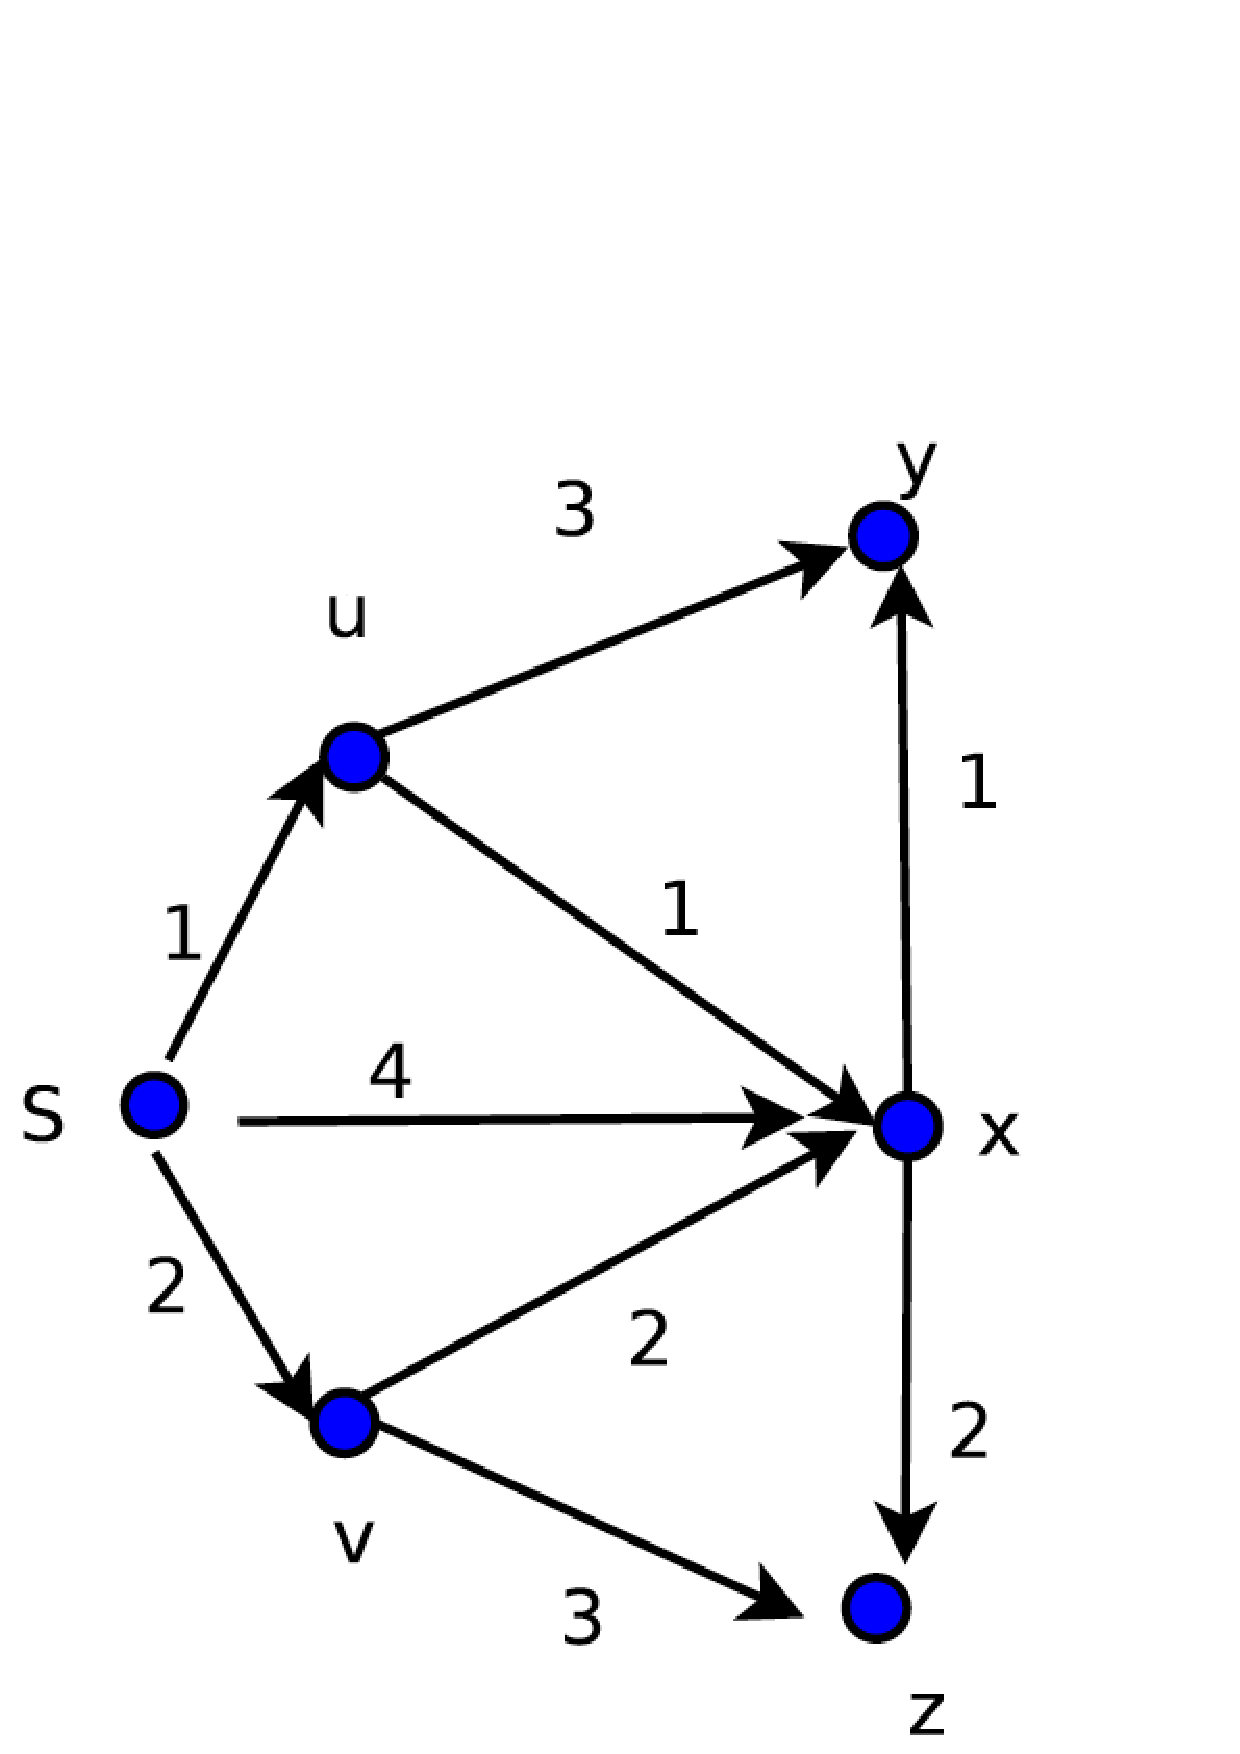
\includegraphics[width=0.9\textwidth]{L7-shortestpathexample.png}
 
\begin{tikzpicture}[auto,swap,scale=0.85]
% 
%    \foreach \pos/\name in {{(0,0)/s}, {(2,2)/u}, {(2,-2)/v}, {(5,0)/x}, {(5,-3)/z}, {(5,3)/y}}
%        \node[vertex,fill=blue!20] (\name) at \pos {$\name$};
%        
%        
%    \foreach \source/\dest/\weight in {s/u/1, s/v/2, s/x/4,   u/y/3,  u/x/1, x/y/1, v/x/2, v/z/3, x/z/2 } 
%            \path[edge] (\source) -- node[weight] {\tiny $\weight$} (\dest);
%	
%\end{tikzpicture} 
%		

  	\def\dx{-6};
 	\def\dy{-1.25};	
    \foreach \pos/\name in {{(0+\dx,0+\dy)/s}, {(2+\dx,1.4+\dy)/u}, {(2+\dx,-1.4+\dy)/v}, {(4+\dx,0+\dy)/x}, {(4+\dx,-2.5+\dy)/t}, {(4+\dx,2.5+\dy)/y}}
        \node[middlevertex,fill=blue!20] (\name) at \pos {$\name$};
        
        
    \foreach \source/\dest/\weight in {s/u/1, s/v/2, s/x/4,   u/y/3,  u/x/1, x/y/1, v/x/2, v/t/3, x/t/2 } 
            \path[edge] (\source) -- node[weight] {\small $\weight$} (\dest);
	
 
% \end{minipage}
% \begin{minipage}{0.45\textwidth}

%  \includegraphics[width=\textwidth]{L7-Dijkstraexample.png}
 
 %\begin{tikzpicture}[scale=0.8, auto,swap]
  
  	\def\d{0.8};
	
	%draw index 
 \def\dy{1};
 \def\dx{0};

    \foreach \i/\num/\name in { 1/k=0/, 2/1/s1,3/2/s2,4/3/s3,5/4/s4,6/5/}{
           \node[blue,thick] (\name) at (\i*\d+\d/2 + \dx*\d - \d, \d/2 + \dy * \d) {\tt \num};
    }

 \def\dy{0};
 \def\dx{0};
    \foreach \i/\num/\name in { 1/s/s1,2/u/s2,3/v/s3,4/x/s4, 5/y/,6/t/}{
         \node[blue,thick] (\name) at ( -1*\d+\d/2,  0.0 - \i*\d + \d/2 - \dy * \d + \d){$\num$};
    }

    
%score	
 \def\dy{0};
 \def\dx{0};
    \foreach \i/\num/\name in { 1/0/S1,2/0/S2,3/0/,4/0/,5/0/}{
             \draw[  thick, fill=green!10 ] (\i*\d + \dx*\d,  0+ \dy*\d) rectangle (\i*\d+\d + \dx*\d, \d + \dy*\d);
    }
    \foreach \i/\num/\name in { 0/0/S0,1/0/S1,2/0/S2,3/0/,4/0/,5/0/}{
             \draw[  thick ] (\i*\d + \dx*\d,  0+ \dy*\d) rectangle (\i*\d+\d + \dx*\d, \d + \dy*\d);
         \node (\name) at (\i*\d+\d/2 + \dx*\d, \d/2 + \dy*\d) {\small $\num$};
    }

      \draw[red,ultra thick] (S0) circle[radius=\d/2];


%   \draw[blue,ultra thick] (S1) circle[radius=\d/2];
%   \draw[blue,ultra thick] (S2) circle[radius=\d/2];
%   \draw[blue,ultra thick] (L) circle[radius=\d/2];
%
    
  
%draw blue rectangles 

 \def\dy{-1};
 \def\dx{0};
    \foreach \i/\num/\name in { 2/1/,3/1/S3,4/1/,5/1/}{
             \draw[  thick, green, fill=green!10 ] (\i*\d + \dx*\d,  0+ \dy*\d) rectangle (\i*\d+\d + \dx*\d, \d + \dy*\d);
    }
 
     
    
 \def\dy{-2};
 \def\dx{0};
    \foreach \i/\num/\name in { 3/2/S3,4/2/,5/2/}{
             \draw[  thick, green, fill=green!10  ] (\i*\d + \dx*\d,  0+ \dy*\d) rectangle (\i*\d+\d + \dx*\d, \d + \dy*\d);
      }
 
    
  \def\dy{-3};
 \def\dx{0};
    \foreach \i/\num/\name in { 3/2/S3,4/2/,5/2/}{
             \draw[  thick, green, fill=green!10 ] (\i*\d + \dx*\d,  0+ \dy*\d) rectangle (\i*\d+\d + \dx*\d, \d + \dy*\d);
    }
 
   \def\dy{-4};
 \def\dx{0};
    \foreach \i/\num/\name in { 4/3/,5/3/}{
             \draw[  thick, green, fill=green!10 ] (\i*\d + \dx*\d,  0+ \dy*\d) rectangle (\i*\d+\d + \dx*\d, \d + \dy*\d);
    }
 
  \def\dy{-5};
 \def\dx{0};
    \foreach \i/\num/\name in {5/4/}{
             \draw[  thick, green, fill=green!10 ] (\i*\d + \dx*\d,  0+ \dy*\d) rectangle (\i*\d+\d + \dx*\d, \d + \dy*\d);
     }
  
       
 \def\dy{-1};
 \def\dx{0};
    \foreach \i/\num/\name in { 0/\infty/,1/1/S1,2/1/,3/1/S3,4/1/,5/1/}{
             \draw[  thick ] (\i*\d + \dx*\d,  0+ \dy*\d) rectangle (\i*\d+\d + \dx*\d, \d + \dy*\d);
         \node (\name) at (\i*\d+\d/2 + \dx*\d, \d/2 + \dy*\d) {\small $\num$};
    }
 
      \draw[red,ultra thick] (S1) circle[radius=\d/2];
   
    
 \def\dy{-2};
 \def\dx{0};
    \foreach \i/\num/\name in { 0/\infty/,1/2/,2/2/S1,3/2/S3,4/2/,5/2/}{
             \draw[  thick ] (\i*\d + \dx*\d,  0+ \dy*\d) rectangle (\i*\d+\d + \dx*\d, \d + \dy*\d);
         \node (\name) at (\i*\d+\d/2 + \dx*\d, \d/2 + \dy*\d) {\small $\num$};
    }
       \draw[red,ultra thick] (S1) circle[radius=\d/2];
 
    
  \def\dy{-3};
 \def\dx{0};
    \foreach \i/\num/\name in { 0/\infty/,1/4/,2/2/S1,3/2/S3,4/2/,5/2/}{
             \draw[  thick ] (\i*\d + \dx*\d,  0+ \dy*\d) rectangle (\i*\d+\d + \dx*\d, \d + \dy*\d);
         \node (\name) at (\i*\d+\d/2 + \dx*\d, \d/2 + \dy*\d) {\small $\num$};
    }
       \draw[red,ultra thick] (S1) circle[radius=\d/2];
  
  \def\dy{-4};
 \def\dx{0};
    \foreach \i/\num/\name in { 0/\infty/,1/\infty/,2/4/,3/3/S1,4/3/,5/3/}{
             \draw[  thick ] (\i*\d + \dx*\d,  0+ \dy*\d) rectangle (\i*\d+\d + \dx*\d, \d + \dy*\d);
         \node (\name) at (\i*\d+\d/2 + \dx*\d, \d/2 + \dy*\d) {\small $\num$};
    }
         \draw[red,ultra thick] (S1) circle[radius=\d/2];

  \def\dy{-5};
 \def\dx{0};
    \foreach \i/\num/\name in { 0/\infty/,1/\infty/,2/5/,3/4/S3,4/4/S1,5/4/}{
             \draw[  thick ] (\i*\d + \dx*\d,  0+ \dy*\d) rectangle (\i*\d+\d + \dx*\d, \d + \dy*\d);
         \node (\name) at (\i*\d+\d/2 + \dx*\d, \d/2 + \dy*\d) {\small $\num$};
    }
        \draw[red,ultra thick] (S1) circle[radius=\d/2];
 


\end{tikzpicture} 
% \caption{\fangsong 在边上的权全为正数的图上{\sc Bellman-Ford}算法运行过程示例。 图中的圆圈内单元表示每一列的最小值(除此前各列最小值之外),阴影区单元与左侧圆圈内单元具有相同的值,因此无需重复进行计算}
\label{vk}
% \end{minipage}
\end{figure}

}

\end{document} 
